\documentclass[11pt]{article}

    \usepackage[breakable]{tcolorbox}
    \usepackage{parskip} % Stop auto-indenting (to mimic markdown behaviour)
    
    \usepackage{iftex}
    \ifPDFTeX
    	\usepackage[T1]{fontenc}
    	\usepackage{mathpazo}
    \else
    	\usepackage{fontspec}
    \fi

    % Basic figure setup, for now with no caption control since it's done
    % automatically by Pandoc (which extracts ![](path) syntax from Markdown).
    \usepackage{graphicx}
    % Maintain compatibility with old templates. Remove in nbconvert 6.0
    \let\Oldincludegraphics\includegraphics
    % Ensure that by default, figures have no caption (until we provide a
    % proper Figure object with a Caption API and a way to capture that
    % in the conversion process - todo).
    \usepackage{caption}
    \DeclareCaptionFormat{nocaption}{}
    \captionsetup{format=nocaption,aboveskip=0pt,belowskip=0pt}

    \usepackage{float}
    \floatplacement{figure}{H} % forces figures to be placed at the correct location
    \usepackage{xcolor} % Allow colors to be defined
    \usepackage{enumerate} % Needed for markdown enumerations to work
    \usepackage{geometry} % Used to adjust the document margins
    \usepackage{amsmath} % Equations
    \usepackage{amssymb} % Equations
    \usepackage{textcomp} % defines textquotesingle
    % Hack from http://tex.stackexchange.com/a/47451/13684:
    \AtBeginDocument{%
        \def\PYZsq{\textquotesingle}% Upright quotes in Pygmentized code
    }
    \usepackage{upquote} % Upright quotes for verbatim code
    \usepackage{eurosym} % defines \euro
    \usepackage[mathletters]{ucs} % Extended unicode (utf-8) support
    \usepackage{fancyvrb} % verbatim replacement that allows latex
    \usepackage{grffile} % extends the file name processing of package graphics 
                         % to support a larger range
    \makeatletter % fix for old versions of grffile with XeLaTeX
    \@ifpackagelater{grffile}{2019/11/01}
    {
      % Do nothing on new versions
    }
    {
      \def\Gread@@xetex#1{%
        \IfFileExists{"\Gin@base".bb}%
        {\Gread@eps{\Gin@base.bb}}%
        {\Gread@@xetex@aux#1}%
      }
    }
    \makeatother
    \usepackage[Export]{adjustbox} % Used to constrain images to a maximum size
    \adjustboxset{max size={0.9\linewidth}{0.9\paperheight}}

    % The hyperref package gives us a pdf with properly built
    % internal navigation ('pdf bookmarks' for the table of contents,
    % internal cross-reference links, web links for URLs, etc.)
    \usepackage{hyperref}
    % The default LaTeX title has an obnoxious amount of whitespace. By default,
    % titling removes some of it. It also provides customization options.
    \usepackage{titling}
    \usepackage{longtable} % longtable support required by pandoc >1.10
    \usepackage{booktabs}  % table support for pandoc > 1.12.2
    \usepackage[inline]{enumitem} % IRkernel/repr support (it uses the enumerate* environment)
    \usepackage[normalem]{ulem} % ulem is needed to support strikethroughs (\sout)
                                % normalem makes italics be italics, not underlines
    \usepackage{mathrsfs}
    

    
    % Colors for the hyperref package
    \definecolor{urlcolor}{rgb}{0,.145,.698}
    \definecolor{linkcolor}{rgb}{.71,0.21,0.01}
    \definecolor{citecolor}{rgb}{.12,.54,.11}

    % ANSI colors
    \definecolor{ansi-black}{HTML}{3E424D}
    \definecolor{ansi-black-intense}{HTML}{282C36}
    \definecolor{ansi-red}{HTML}{E75C58}
    \definecolor{ansi-red-intense}{HTML}{B22B31}
    \definecolor{ansi-green}{HTML}{00A250}
    \definecolor{ansi-green-intense}{HTML}{007427}
    \definecolor{ansi-yellow}{HTML}{DDB62B}
    \definecolor{ansi-yellow-intense}{HTML}{B27D12}
    \definecolor{ansi-blue}{HTML}{208FFB}
    \definecolor{ansi-blue-intense}{HTML}{0065CA}
    \definecolor{ansi-magenta}{HTML}{D160C4}
    \definecolor{ansi-magenta-intense}{HTML}{A03196}
    \definecolor{ansi-cyan}{HTML}{60C6C8}
    \definecolor{ansi-cyan-intense}{HTML}{258F8F}
    \definecolor{ansi-white}{HTML}{C5C1B4}
    \definecolor{ansi-white-intense}{HTML}{A1A6B2}
    \definecolor{ansi-default-inverse-fg}{HTML}{FFFFFF}
    \definecolor{ansi-default-inverse-bg}{HTML}{000000}

    % common color for the border for error outputs.
    \definecolor{outerrorbackground}{HTML}{FFDFDF}

    % commands and environments needed by pandoc snippets
    % extracted from the output of `pandoc -s`
    \providecommand{\tightlist}{%
      \setlength{\itemsep}{0pt}\setlength{\parskip}{0pt}}
    \DefineVerbatimEnvironment{Highlighting}{Verbatim}{commandchars=\\\{\}}
    % Add ',fontsize=\small' for more characters per line
    \newenvironment{Shaded}{}{}
    \newcommand{\KeywordTok}[1]{\textcolor[rgb]{0.00,0.44,0.13}{\textbf{{#1}}}}
    \newcommand{\DataTypeTok}[1]{\textcolor[rgb]{0.56,0.13,0.00}{{#1}}}
    \newcommand{\DecValTok}[1]{\textcolor[rgb]{0.25,0.63,0.44}{{#1}}}
    \newcommand{\BaseNTok}[1]{\textcolor[rgb]{0.25,0.63,0.44}{{#1}}}
    \newcommand{\FloatTok}[1]{\textcolor[rgb]{0.25,0.63,0.44}{{#1}}}
    \newcommand{\CharTok}[1]{\textcolor[rgb]{0.25,0.44,0.63}{{#1}}}
    \newcommand{\StringTok}[1]{\textcolor[rgb]{0.25,0.44,0.63}{{#1}}}
    \newcommand{\CommentTok}[1]{\textcolor[rgb]{0.38,0.63,0.69}{\textit{{#1}}}}
    \newcommand{\OtherTok}[1]{\textcolor[rgb]{0.00,0.44,0.13}{{#1}}}
    \newcommand{\AlertTok}[1]{\textcolor[rgb]{1.00,0.00,0.00}{\textbf{{#1}}}}
    \newcommand{\FunctionTok}[1]{\textcolor[rgb]{0.02,0.16,0.49}{{#1}}}
    \newcommand{\RegionMarkerTok}[1]{{#1}}
    \newcommand{\ErrorTok}[1]{\textcolor[rgb]{1.00,0.00,0.00}{\textbf{{#1}}}}
    \newcommand{\NormalTok}[1]{{#1}}
    
    % Additional commands for more recent versions of Pandoc
    \newcommand{\ConstantTok}[1]{\textcolor[rgb]{0.53,0.00,0.00}{{#1}}}
    \newcommand{\SpecialCharTok}[1]{\textcolor[rgb]{0.25,0.44,0.63}{{#1}}}
    \newcommand{\VerbatimStringTok}[1]{\textcolor[rgb]{0.25,0.44,0.63}{{#1}}}
    \newcommand{\SpecialStringTok}[1]{\textcolor[rgb]{0.73,0.40,0.53}{{#1}}}
    \newcommand{\ImportTok}[1]{{#1}}
    \newcommand{\DocumentationTok}[1]{\textcolor[rgb]{0.73,0.13,0.13}{\textit{{#1}}}}
    \newcommand{\AnnotationTok}[1]{\textcolor[rgb]{0.38,0.63,0.69}{\textbf{\textit{{#1}}}}}
    \newcommand{\CommentVarTok}[1]{\textcolor[rgb]{0.38,0.63,0.69}{\textbf{\textit{{#1}}}}}
    \newcommand{\VariableTok}[1]{\textcolor[rgb]{0.10,0.09,0.49}{{#1}}}
    \newcommand{\ControlFlowTok}[1]{\textcolor[rgb]{0.00,0.44,0.13}{\textbf{{#1}}}}
    \newcommand{\OperatorTok}[1]{\textcolor[rgb]{0.40,0.40,0.40}{{#1}}}
    \newcommand{\BuiltInTok}[1]{{#1}}
    \newcommand{\ExtensionTok}[1]{{#1}}
    \newcommand{\PreprocessorTok}[1]{\textcolor[rgb]{0.74,0.48,0.00}{{#1}}}
    \newcommand{\AttributeTok}[1]{\textcolor[rgb]{0.49,0.56,0.16}{{#1}}}
    \newcommand{\InformationTok}[1]{\textcolor[rgb]{0.38,0.63,0.69}{\textbf{\textit{{#1}}}}}
    \newcommand{\WarningTok}[1]{\textcolor[rgb]{0.38,0.63,0.69}{\textbf{\textit{{#1}}}}}
    
    
    % Define a nice break command that doesn't care if a line doesn't already
    % exist.
    \def\br{\hspace*{\fill} \\* }
    % Math Jax compatibility definitions
    \def\gt{>}
    \def\lt{<}
    \let\Oldtex\TeX
    \let\Oldlatex\LaTeX
    \renewcommand{\TeX}{\textrm{\Oldtex}}
    \renewcommand{\LaTeX}{\textrm{\Oldlatex}}
    % Document parameters
    % Document title
    \title{SWNM}
    
    
    
    
    
% Pygments definitions
\makeatletter
\def\PY@reset{\let\PY@it=\relax \let\PY@bf=\relax%
    \let\PY@ul=\relax \let\PY@tc=\relax%
    \let\PY@bc=\relax \let\PY@ff=\relax}
\def\PY@tok#1{\csname PY@tok@#1\endcsname}
\def\PY@toks#1+{\ifx\relax#1\empty\else%
    \PY@tok{#1}\expandafter\PY@toks\fi}
\def\PY@do#1{\PY@bc{\PY@tc{\PY@ul{%
    \PY@it{\PY@bf{\PY@ff{#1}}}}}}}
\def\PY#1#2{\PY@reset\PY@toks#1+\relax+\PY@do{#2}}

\@namedef{PY@tok@w}{\def\PY@tc##1{\textcolor[rgb]{0.73,0.73,0.73}{##1}}}
\@namedef{PY@tok@c}{\let\PY@it=\textit\def\PY@tc##1{\textcolor[rgb]{0.25,0.50,0.50}{##1}}}
\@namedef{PY@tok@cp}{\def\PY@tc##1{\textcolor[rgb]{0.74,0.48,0.00}{##1}}}
\@namedef{PY@tok@k}{\let\PY@bf=\textbf\def\PY@tc##1{\textcolor[rgb]{0.00,0.50,0.00}{##1}}}
\@namedef{PY@tok@kp}{\def\PY@tc##1{\textcolor[rgb]{0.00,0.50,0.00}{##1}}}
\@namedef{PY@tok@kt}{\def\PY@tc##1{\textcolor[rgb]{0.69,0.00,0.25}{##1}}}
\@namedef{PY@tok@o}{\def\PY@tc##1{\textcolor[rgb]{0.40,0.40,0.40}{##1}}}
\@namedef{PY@tok@ow}{\let\PY@bf=\textbf\def\PY@tc##1{\textcolor[rgb]{0.67,0.13,1.00}{##1}}}
\@namedef{PY@tok@nb}{\def\PY@tc##1{\textcolor[rgb]{0.00,0.50,0.00}{##1}}}
\@namedef{PY@tok@nf}{\def\PY@tc##1{\textcolor[rgb]{0.00,0.00,1.00}{##1}}}
\@namedef{PY@tok@nc}{\let\PY@bf=\textbf\def\PY@tc##1{\textcolor[rgb]{0.00,0.00,1.00}{##1}}}
\@namedef{PY@tok@nn}{\let\PY@bf=\textbf\def\PY@tc##1{\textcolor[rgb]{0.00,0.00,1.00}{##1}}}
\@namedef{PY@tok@ne}{\let\PY@bf=\textbf\def\PY@tc##1{\textcolor[rgb]{0.82,0.25,0.23}{##1}}}
\@namedef{PY@tok@nv}{\def\PY@tc##1{\textcolor[rgb]{0.10,0.09,0.49}{##1}}}
\@namedef{PY@tok@no}{\def\PY@tc##1{\textcolor[rgb]{0.53,0.00,0.00}{##1}}}
\@namedef{PY@tok@nl}{\def\PY@tc##1{\textcolor[rgb]{0.63,0.63,0.00}{##1}}}
\@namedef{PY@tok@ni}{\let\PY@bf=\textbf\def\PY@tc##1{\textcolor[rgb]{0.60,0.60,0.60}{##1}}}
\@namedef{PY@tok@na}{\def\PY@tc##1{\textcolor[rgb]{0.49,0.56,0.16}{##1}}}
\@namedef{PY@tok@nt}{\let\PY@bf=\textbf\def\PY@tc##1{\textcolor[rgb]{0.00,0.50,0.00}{##1}}}
\@namedef{PY@tok@nd}{\def\PY@tc##1{\textcolor[rgb]{0.67,0.13,1.00}{##1}}}
\@namedef{PY@tok@s}{\def\PY@tc##1{\textcolor[rgb]{0.73,0.13,0.13}{##1}}}
\@namedef{PY@tok@sd}{\let\PY@it=\textit\def\PY@tc##1{\textcolor[rgb]{0.73,0.13,0.13}{##1}}}
\@namedef{PY@tok@si}{\let\PY@bf=\textbf\def\PY@tc##1{\textcolor[rgb]{0.73,0.40,0.53}{##1}}}
\@namedef{PY@tok@se}{\let\PY@bf=\textbf\def\PY@tc##1{\textcolor[rgb]{0.73,0.40,0.13}{##1}}}
\@namedef{PY@tok@sr}{\def\PY@tc##1{\textcolor[rgb]{0.73,0.40,0.53}{##1}}}
\@namedef{PY@tok@ss}{\def\PY@tc##1{\textcolor[rgb]{0.10,0.09,0.49}{##1}}}
\@namedef{PY@tok@sx}{\def\PY@tc##1{\textcolor[rgb]{0.00,0.50,0.00}{##1}}}
\@namedef{PY@tok@m}{\def\PY@tc##1{\textcolor[rgb]{0.40,0.40,0.40}{##1}}}
\@namedef{PY@tok@gh}{\let\PY@bf=\textbf\def\PY@tc##1{\textcolor[rgb]{0.00,0.00,0.50}{##1}}}
\@namedef{PY@tok@gu}{\let\PY@bf=\textbf\def\PY@tc##1{\textcolor[rgb]{0.50,0.00,0.50}{##1}}}
\@namedef{PY@tok@gd}{\def\PY@tc##1{\textcolor[rgb]{0.63,0.00,0.00}{##1}}}
\@namedef{PY@tok@gi}{\def\PY@tc##1{\textcolor[rgb]{0.00,0.63,0.00}{##1}}}
\@namedef{PY@tok@gr}{\def\PY@tc##1{\textcolor[rgb]{1.00,0.00,0.00}{##1}}}
\@namedef{PY@tok@ge}{\let\PY@it=\textit}
\@namedef{PY@tok@gs}{\let\PY@bf=\textbf}
\@namedef{PY@tok@gp}{\let\PY@bf=\textbf\def\PY@tc##1{\textcolor[rgb]{0.00,0.00,0.50}{##1}}}
\@namedef{PY@tok@go}{\def\PY@tc##1{\textcolor[rgb]{0.53,0.53,0.53}{##1}}}
\@namedef{PY@tok@gt}{\def\PY@tc##1{\textcolor[rgb]{0.00,0.27,0.87}{##1}}}
\@namedef{PY@tok@err}{\def\PY@bc##1{{\setlength{\fboxsep}{-\fboxrule}\fcolorbox[rgb]{1.00,0.00,0.00}{1,1,1}{\strut ##1}}}}
\@namedef{PY@tok@kc}{\let\PY@bf=\textbf\def\PY@tc##1{\textcolor[rgb]{0.00,0.50,0.00}{##1}}}
\@namedef{PY@tok@kd}{\let\PY@bf=\textbf\def\PY@tc##1{\textcolor[rgb]{0.00,0.50,0.00}{##1}}}
\@namedef{PY@tok@kn}{\let\PY@bf=\textbf\def\PY@tc##1{\textcolor[rgb]{0.00,0.50,0.00}{##1}}}
\@namedef{PY@tok@kr}{\let\PY@bf=\textbf\def\PY@tc##1{\textcolor[rgb]{0.00,0.50,0.00}{##1}}}
\@namedef{PY@tok@bp}{\def\PY@tc##1{\textcolor[rgb]{0.00,0.50,0.00}{##1}}}
\@namedef{PY@tok@fm}{\def\PY@tc##1{\textcolor[rgb]{0.00,0.00,1.00}{##1}}}
\@namedef{PY@tok@vc}{\def\PY@tc##1{\textcolor[rgb]{0.10,0.09,0.49}{##1}}}
\@namedef{PY@tok@vg}{\def\PY@tc##1{\textcolor[rgb]{0.10,0.09,0.49}{##1}}}
\@namedef{PY@tok@vi}{\def\PY@tc##1{\textcolor[rgb]{0.10,0.09,0.49}{##1}}}
\@namedef{PY@tok@vm}{\def\PY@tc##1{\textcolor[rgb]{0.10,0.09,0.49}{##1}}}
\@namedef{PY@tok@sa}{\def\PY@tc##1{\textcolor[rgb]{0.73,0.13,0.13}{##1}}}
\@namedef{PY@tok@sb}{\def\PY@tc##1{\textcolor[rgb]{0.73,0.13,0.13}{##1}}}
\@namedef{PY@tok@sc}{\def\PY@tc##1{\textcolor[rgb]{0.73,0.13,0.13}{##1}}}
\@namedef{PY@tok@dl}{\def\PY@tc##1{\textcolor[rgb]{0.73,0.13,0.13}{##1}}}
\@namedef{PY@tok@s2}{\def\PY@tc##1{\textcolor[rgb]{0.73,0.13,0.13}{##1}}}
\@namedef{PY@tok@sh}{\def\PY@tc##1{\textcolor[rgb]{0.73,0.13,0.13}{##1}}}
\@namedef{PY@tok@s1}{\def\PY@tc##1{\textcolor[rgb]{0.73,0.13,0.13}{##1}}}
\@namedef{PY@tok@mb}{\def\PY@tc##1{\textcolor[rgb]{0.40,0.40,0.40}{##1}}}
\@namedef{PY@tok@mf}{\def\PY@tc##1{\textcolor[rgb]{0.40,0.40,0.40}{##1}}}
\@namedef{PY@tok@mh}{\def\PY@tc##1{\textcolor[rgb]{0.40,0.40,0.40}{##1}}}
\@namedef{PY@tok@mi}{\def\PY@tc##1{\textcolor[rgb]{0.40,0.40,0.40}{##1}}}
\@namedef{PY@tok@il}{\def\PY@tc##1{\textcolor[rgb]{0.40,0.40,0.40}{##1}}}
\@namedef{PY@tok@mo}{\def\PY@tc##1{\textcolor[rgb]{0.40,0.40,0.40}{##1}}}
\@namedef{PY@tok@ch}{\let\PY@it=\textit\def\PY@tc##1{\textcolor[rgb]{0.25,0.50,0.50}{##1}}}
\@namedef{PY@tok@cm}{\let\PY@it=\textit\def\PY@tc##1{\textcolor[rgb]{0.25,0.50,0.50}{##1}}}
\@namedef{PY@tok@cpf}{\let\PY@it=\textit\def\PY@tc##1{\textcolor[rgb]{0.25,0.50,0.50}{##1}}}
\@namedef{PY@tok@c1}{\let\PY@it=\textit\def\PY@tc##1{\textcolor[rgb]{0.25,0.50,0.50}{##1}}}
\@namedef{PY@tok@cs}{\let\PY@it=\textit\def\PY@tc##1{\textcolor[rgb]{0.25,0.50,0.50}{##1}}}

\def\PYZbs{\char`\\}
\def\PYZus{\char`\_}
\def\PYZob{\char`\{}
\def\PYZcb{\char`\}}
\def\PYZca{\char`\^}
\def\PYZam{\char`\&}
\def\PYZlt{\char`\<}
\def\PYZgt{\char`\>}
\def\PYZsh{\char`\#}
\def\PYZpc{\char`\%}
\def\PYZdl{\char`\$}
\def\PYZhy{\char`\-}
\def\PYZsq{\char`\'}
\def\PYZdq{\char`\"}
\def\PYZti{\char`\~}
% for compatibility with earlier versions
\def\PYZat{@}
\def\PYZlb{[}
\def\PYZrb{]}
\makeatother


    % For linebreaks inside Verbatim environment from package fancyvrb. 
    \makeatletter
        \newbox\Wrappedcontinuationbox 
        \newbox\Wrappedvisiblespacebox 
        \newcommand*\Wrappedvisiblespace {\textcolor{red}{\textvisiblespace}} 
        \newcommand*\Wrappedcontinuationsymbol {\textcolor{red}{\llap{\tiny$\m@th\hookrightarrow$}}} 
        \newcommand*\Wrappedcontinuationindent {3ex } 
        \newcommand*\Wrappedafterbreak {\kern\Wrappedcontinuationindent\copy\Wrappedcontinuationbox} 
        % Take advantage of the already applied Pygments mark-up to insert 
        % potential linebreaks for TeX processing. 
        %        {, <, #, %, $, ' and ": go to next line. 
        %        _, }, ^, &, >, - and ~: stay at end of broken line. 
        % Use of \textquotesingle for straight quote. 
        \newcommand*\Wrappedbreaksatspecials {% 
            \def\PYGZus{\discretionary{\char`\_}{\Wrappedafterbreak}{\char`\_}}% 
            \def\PYGZob{\discretionary{}{\Wrappedafterbreak\char`\{}{\char`\{}}% 
            \def\PYGZcb{\discretionary{\char`\}}{\Wrappedafterbreak}{\char`\}}}% 
            \def\PYGZca{\discretionary{\char`\^}{\Wrappedafterbreak}{\char`\^}}% 
            \def\PYGZam{\discretionary{\char`\&}{\Wrappedafterbreak}{\char`\&}}% 
            \def\PYGZlt{\discretionary{}{\Wrappedafterbreak\char`\<}{\char`\<}}% 
            \def\PYGZgt{\discretionary{\char`\>}{\Wrappedafterbreak}{\char`\>}}% 
            \def\PYGZsh{\discretionary{}{\Wrappedafterbreak\char`\#}{\char`\#}}% 
            \def\PYGZpc{\discretionary{}{\Wrappedafterbreak\char`\%}{\char`\%}}% 
            \def\PYGZdl{\discretionary{}{\Wrappedafterbreak\char`\$}{\char`\$}}% 
            \def\PYGZhy{\discretionary{\char`\-}{\Wrappedafterbreak}{\char`\-}}% 
            \def\PYGZsq{\discretionary{}{\Wrappedafterbreak\textquotesingle}{\textquotesingle}}% 
            \def\PYGZdq{\discretionary{}{\Wrappedafterbreak\char`\"}{\char`\"}}% 
            \def\PYGZti{\discretionary{\char`\~}{\Wrappedafterbreak}{\char`\~}}% 
        } 
        % Some characters . , ; ? ! / are not pygmentized. 
        % This macro makes them "active" and they will insert potential linebreaks 
        \newcommand*\Wrappedbreaksatpunct {% 
            \lccode`\~`\.\lowercase{\def~}{\discretionary{\hbox{\char`\.}}{\Wrappedafterbreak}{\hbox{\char`\.}}}% 
            \lccode`\~`\,\lowercase{\def~}{\discretionary{\hbox{\char`\,}}{\Wrappedafterbreak}{\hbox{\char`\,}}}% 
            \lccode`\~`\;\lowercase{\def~}{\discretionary{\hbox{\char`\;}}{\Wrappedafterbreak}{\hbox{\char`\;}}}% 
            \lccode`\~`\:\lowercase{\def~}{\discretionary{\hbox{\char`\:}}{\Wrappedafterbreak}{\hbox{\char`\:}}}% 
            \lccode`\~`\?\lowercase{\def~}{\discretionary{\hbox{\char`\?}}{\Wrappedafterbreak}{\hbox{\char`\?}}}% 
            \lccode`\~`\!\lowercase{\def~}{\discretionary{\hbox{\char`\!}}{\Wrappedafterbreak}{\hbox{\char`\!}}}% 
            \lccode`\~`\/\lowercase{\def~}{\discretionary{\hbox{\char`\/}}{\Wrappedafterbreak}{\hbox{\char`\/}}}% 
            \catcode`\.\active
            \catcode`\,\active 
            \catcode`\;\active
            \catcode`\:\active
            \catcode`\?\active
            \catcode`\!\active
            \catcode`\/\active 
            \lccode`\~`\~ 	
        }
    \makeatother

    \let\OriginalVerbatim=\Verbatim
    \makeatletter
    \renewcommand{\Verbatim}[1][1]{%
        %\parskip\z@skip
        \sbox\Wrappedcontinuationbox {\Wrappedcontinuationsymbol}%
        \sbox\Wrappedvisiblespacebox {\FV@SetupFont\Wrappedvisiblespace}%
        \def\FancyVerbFormatLine ##1{\hsize\linewidth
            \vtop{\raggedright\hyphenpenalty\z@\exhyphenpenalty\z@
                \doublehyphendemerits\z@\finalhyphendemerits\z@
                \strut ##1\strut}%
        }%
        % If the linebreak is at a space, the latter will be displayed as visible
        % space at end of first line, and a continuation symbol starts next line.
        % Stretch/shrink are however usually zero for typewriter font.
        \def\FV@Space {%
            \nobreak\hskip\z@ plus\fontdimen3\font minus\fontdimen4\font
            \discretionary{\copy\Wrappedvisiblespacebox}{\Wrappedafterbreak}
            {\kern\fontdimen2\font}%
        }%
        
        % Allow breaks at special characters using \PYG... macros.
        \Wrappedbreaksatspecials
        % Breaks at punctuation characters . , ; ? ! and / need catcode=\active 	
        \OriginalVerbatim[#1,codes*=\Wrappedbreaksatpunct]%
    }
    \makeatother

    % Exact colors from NB
    \definecolor{incolor}{HTML}{303F9F}
    \definecolor{outcolor}{HTML}{D84315}
    \definecolor{cellborder}{HTML}{CFCFCF}
    \definecolor{cellbackground}{HTML}{F7F7F7}
    
    % prompt
    \makeatletter
    \newcommand{\boxspacing}{\kern\kvtcb@left@rule\kern\kvtcb@boxsep}
    \makeatother
    \newcommand{\prompt}[4]{
        {\ttfamily\llap{{\color{#2}[#3]:\hspace{3pt}#4}}\vspace{-\baselineskip}}
    }
    

    
    % Prevent overflowing lines due to hard-to-break entities
    \sloppy 
    % Setup hyperref package
    \hypersetup{
      breaklinks=true,  % so long urls are correctly broken across lines
      colorlinks=true,
      urlcolor=urlcolor,
      linkcolor=linkcolor,
      citecolor=citecolor,
      }
    % Slightly bigger margins than the latex defaults
    
    \geometry{verbose,tmargin=1in,bmargin=1in,lmargin=1in,rmargin=1in}
    
    

\begin{document}
    
    \maketitle
    
    

    
    \hypertarget{geothermal-machine-learning-analysis-southwest-new-mexico}{%
\subsection{Geothermal machine learning analysis: Southwest New
Mexico}\label{geothermal-machine-learning-analysis-southwest-new-mexico}}

This notebook is a part of the GeoThermalCloud.jl: Machine Learning
framework for Geothermal Exploration.

\begin{verbatim}
<img src="../../logos/geothermalcloud-small.png" alt="geothermalcloud" width=25%  max-width=125px;/>
\end{verbatim}

Machine learning analyses are performed using the \textbf{SmartTensors}
machine learning framework.

\begin{verbatim}
<img src="../../logos/SmartTensorsNewSmaller.png" alt="SmartTensors" width=25%  max-width=125px;/>
\end{verbatim}

This notebook demonstrates how the \textbf{NMFk} module of
\textbf{SmartTensors} can be applied to perform unsupervised geothermal
machine-learning analyses.

\begin{verbatim}
<img src="../../logos/nmfk-logo.png" alt="nmfk" width=25%  max-width=125px;/>
\end{verbatim}

More information on how the ML results are interpreted to provide
geothermal insights is discussed in our research paper.

    \hypertarget{introduction}{%
\subsection{Introduction}\label{introduction}}

Southwest New Mexico (\textbf{SWNM}) is a region important for
geothermal exploration.

\textbf{SWNM} is broadly divided into four physiographic provinces: -
the Colorado Plateau - the Mogollon-Datil Volcanic Field (MDVF) - the
Basin and Range, and - the Rio Grande rift.

Each of the \textbf{SWNM} physiographic provinces is associated with
different types of unique hydrothermal systems with temperatures ranging
from low (\textless90℃) to medium (90-150℃).

Some of the \textbf{SWNM} systems are already utilized for commercial
and recreational purposes.

There are already energy-production facilities for both electricity and
direct-use heating.

For example, the Basin and Range province has one geothermal power plant
(Lightning dock) of gross \textasciitilde14 MWe power, five greenhouse
farms, and numerous medium-temperature wells and springs. There are 14
spas and recreational facilities utilizing the \textbf{SWNM} geothermal
resources.

Recent Play Fairway Analysis (PFA) Phase I study of \textbf{SWNM}
conducted at LANL revealed more potential geothermal resources.

The study area and the data collection locations are mapped below.

\begin{figure}
\centering
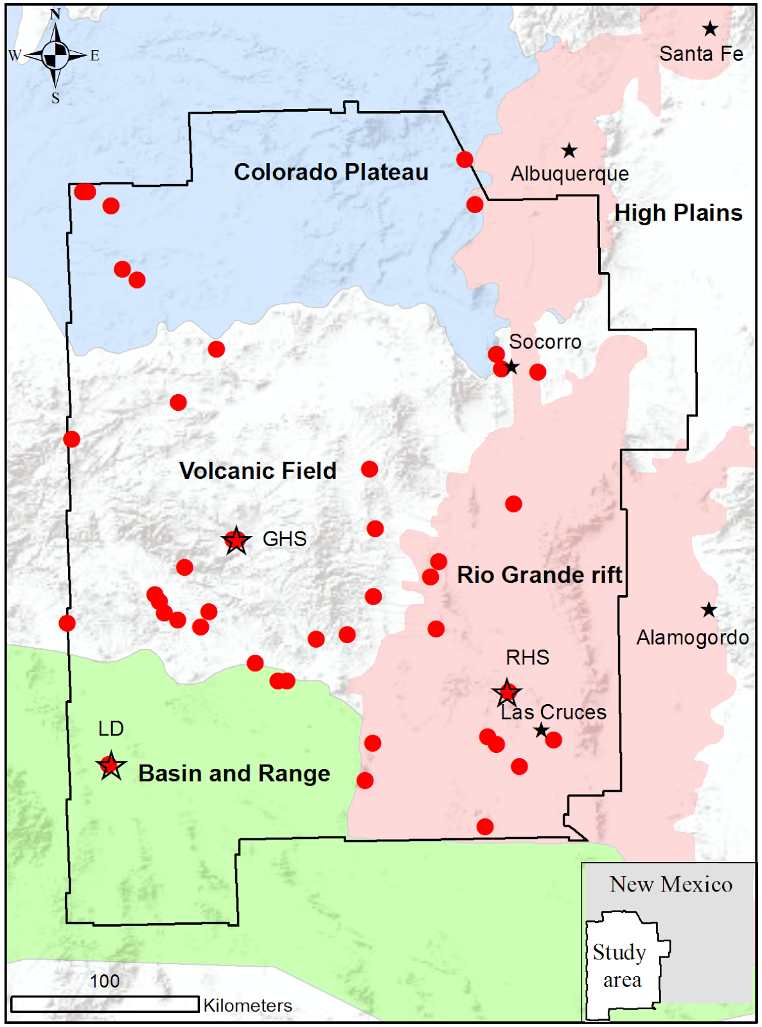
\includegraphics{../map/SWNM_study_area.png}
\caption{SWNM study area}
\end{figure}

    \hypertarget{geothermalcloud-installation}{%
\subsection{GeoThermalCloud
installation}\label{geothermalcloud-installation}}

If \textbf{GeoThermalCloud} is not installed, first execute in the Julia
REPL
\texttt{import\ Pkg;\ Pkg.add("GeoThermalCloud");\ import\ Pkg;\ Pkg.add("NMFk");\ Pkg.add("Mads");\ Pkg.add("DelimitedFiles");\ Pkg.add("JLD");\ Pkg.add("Gadfly");\ Pkg.add("Cairo");\ Pkg.add("Fontconfig")}.

    \begin{tcolorbox}[breakable, size=fbox, boxrule=1pt, pad at break*=1mm,colback=cellbackground, colframe=cellborder]
\prompt{In}{incolor}{1}{\boxspacing}
\begin{Verbatim}[commandchars=\\\{\}]
\PY{k}{import} \PY{n}{GeoThermalCloud}
\PY{k}{import} \PY{n}{NMFk}
\PY{k}{import} \PY{n}{Mads}
\PY{k}{import} \PY{n}{DelimitedFiles}
\PY{k}{import} \PY{n}{JLD}
\PY{k}{import} \PY{n}{Gadfly}
\PY{k}{import} \PY{n}{Cairo}
\PY{k}{import} \PY{n}{Fontconfig}
\end{Verbatim}
\end{tcolorbox}

    
    \begin{Verbatim}[commandchars=\\\{\}]
HTML\{String\}("<script>\textbackslash{}n// Immediately-invoked-function-expression to avoid global variables.\textbackslash{}n(function() \{\textbackslash{}n    var warning\_div = document.getElementById(\textbackslash{}"webio-warning-1871911905836905661\textbackslash{}");\textbackslash{}n    var hide = function () \{\textbackslash{}n        var script = document.getElementById(\textbackslash{}"webio-setup-17652940122857074023\textbackslash{}");\textbackslash{}n        var parent = script \&\& script.parentElement;\textbackslash{}n        var grandparent = parent \&\& parent.parentElement;\textbackslash{}n        if (grandparent) \{\textbackslash{}n            grandparent.style.display = \textbackslash{}"none\textbackslash{}";\textbackslash{}n        \}\textbackslash{}n        warning\_div.style.display = \textbackslash{}"none\textbackslash{}";\textbackslash{}n    \};\textbackslash{}n    if (typeof Jupyter !== \textbackslash{}"undefined\textbackslash{}") \{\textbackslash{}n        console.log(\textbackslash{}"WebIO detected Jupyter notebook environment.\textbackslash{}");\textbackslash{}n        // Jupyter notebook.\textbackslash{}n        var extensions = (\textbackslash{}n            Jupyter\textbackslash{}n            \&\& Jupyter.notebook.config.data\textbackslash{}n            \&\& Jupyter.notebook.config.data.load\_extensions\textbackslash{}n        );\textbackslash{}n        if (extensions \&\& extensions[\textbackslash{}"webio-jupyter-notebook\textbackslash{}"]) \{\textbackslash{}n            // Extension already loaded.\textbackslash{}n            console.log(\textbackslash{}"Jupyter WebIO nbextension detected; not loading ad-hoc.\textbackslash{}");\textbackslash{}n            hide();\textbackslash{}n            return;\textbackslash{}n        \}\textbackslash{}n    \} else if (window.location.pathname.includes(\textbackslash{}"/lab\textbackslash{}")) \{\textbackslash{}n        // Guessing JupyterLa\textbackslash{}n        console.log(\textbackslash{}"Jupyter Lab detected; make sure the @webio/jupyter-lab-provider labextension is installed.\textbackslash{}");\textbackslash{}n        hide();\textbackslash{}n        return;\textbackslash{}n    \}\textbackslash{}n\})();\textbackslash{}n\textbackslash{}n</script>\textbackslash{}n<p\textbackslash{}n    id=\textbackslash{}"webio-warning-1871911905836905661\textbackslash{}"\textbackslash{}n    class=\textbackslash{}"output\_text output\_stderr\textbackslash{}"\textbackslash{}n    style=\textbackslash{}"padding: 1em; font-weight: bold;\textbackslash{}"\textbackslash{}n>\textbackslash{}n    Unable to load WebIO. Please make sure WebIO works for your Jupyter client.\textbackslash{}n    For troubleshooting, please see <a href=\textbackslash{}"https://juliagizmos.github.io/WebIO.jl/latest/providers/ijulia/\textbackslash{}">\textbackslash{}n    the WebIO/IJulia documentation</a>.\textbackslash{}n    <!-- TODO: link to installation docs. -->\textbackslash{}n</p>\textbackslash{}n")
    \end{Verbatim}

    
    \begin{Verbatim}[commandchars=\\\{\}]
┌ Info: Precompiling NMFk [e40cd9e2-a1df-5d90-a1fa-603fdc3dbdd8]
└ @ Base loading.jl:1278
    \end{Verbatim}

    \begin{Verbatim}[commandchars=\\\{\}]
\textbf{NMFk: Nonnegative Matrix Factorization + k-means clustering and physics
constraints}
====

\textcolor{ansi-blue-intense}{\textbf{  \_     \_  }}\textcolor{ansi-red-intense}{\textbf{ \_      \_  }}\textcolor{ansi-green-intense}{\textbf{ \_\_\_\_\_\_\_   }}\textcolor{ansi-magenta-intense}{\textbf{\_}}
\textcolor{ansi-blue-intense}{\textbf{ |  \textbackslash{}  | | }}\textcolor{ansi-red-intense}{\textbf{|  \textbackslash{}  /  | }}\textcolor{ansi-green-intense}{\textbf{|  \_\_\_\_\_| }}\textcolor{ansi-magenta-intense}{\textbf{| |  \_}}
\textcolor{ansi-blue-intense}{\textbf{ | . \textbackslash{} | | }}\textcolor{ansi-red-intense}{\textbf{| . \textbackslash{}/ . | }}\textcolor{ansi-green-intense}{\textbf{| |\_\_\_    }}\textcolor{ansi-magenta-intense}{\textbf{| | / /}}
\textcolor{ansi-blue-intense}{\textbf{ | |\textbackslash{} \textbackslash{}| | }}\textcolor{ansi-red-intense}{\textbf{| |\textbackslash{}  /| | }}\textcolor{ansi-green-intense}{\textbf{|  \_\_\_|   }}\textcolor{ansi-magenta-intense}{\textbf{| |/ /}}
\textcolor{ansi-blue-intense}{\textbf{ | | \textbackslash{} ' | }}\textcolor{ansi-red-intense}{\textbf{| | \textbackslash{}/ | | }}\textcolor{ansi-green-intense}{\textbf{| |       }}\textcolor{ansi-magenta-intense}{\textbf{|   (}}
\textcolor{ansi-blue-intense}{\textbf{ | |  \textbackslash{}  | }}\textcolor{ansi-red-intense}{\textbf{| |    | | }}\textcolor{ansi-green-intense}{\textbf{| |       }}\textcolor{ansi-magenta-intense}{\textbf{| |\textbackslash{} \textbackslash{}}}
\textcolor{ansi-blue-intense}{\textbf{ |\_|   \textbackslash{}\_| }}\textcolor{ansi-red-intense}{\textbf{|\_|    |\_| }}\textcolor{ansi-green-intense}{\textbf{|\_|       }}\textcolor{ansi-magenta-intense}{\textbf{|\_| \textbackslash{}\_\textbackslash{}}}

NMFk performs unsupervised machine learning based on matrix decomposition
coupled with various constraints.
NMFk provides automatic identification of the optimal number of signals
(features) present in two-dimensional data arrays (matrices).
NMFk offers visualization, pre-, and post-processing capabilities.
    \end{Verbatim}

    \begin{Verbatim}[commandchars=\\\{\}]
┌ Info: Installing pyqt package to avoid buggy tkagg backend.
└ @ PyPlot /Users/vvv/.julia/packages/PyPlot/XHEG0/src/init.jl:118
    \end{Verbatim}

    \hypertarget{load-and-pre-process-the-data}{%
\subsection{Load and pre-process the
data}\label{load-and-pre-process-the-data}}

    \hypertarget{setup-the-working-directory-containing-the-swnm-data}{%
\subsubsection{Setup the working directory containing the SWNM
data}\label{setup-the-working-directory-containing-the-swnm-data}}

    \begin{tcolorbox}[breakable, size=fbox, boxrule=1pt, pad at break*=1mm,colback=cellbackground, colframe=cellborder]
\prompt{In}{incolor}{2}{\boxspacing}
\begin{Verbatim}[commandchars=\\\{\}]
\PY{n}{cd}\PY{p}{(}\PY{n}{joinpath}\PY{p}{(}\PY{n}{GeoThermalCloud}\PY{o}{.}\PY{n}{dir}\PY{p}{,} \PY{l+s}{\PYZdq{}}\PY{l+s}{S}\PY{l+s}{W}\PY{l+s}{N}\PY{l+s}{M}\PY{l+s}{\PYZdq{}}\PY{p}{)}\PY{p}{)}
\end{Verbatim}
\end{tcolorbox}

    \hypertarget{load-the-swnm-data-file}{%
\subsubsection{Load the SWNM data file}\label{load-the-swnm-data-file}}

    \begin{tcolorbox}[breakable, size=fbox, boxrule=1pt, pad at break*=1mm,colback=cellbackground, colframe=cellborder]
\prompt{In}{incolor}{3}{\boxspacing}
\begin{Verbatim}[commandchars=\\\{\}]
\PY{n}{d}\PY{p}{,} \PY{n}{h} \PY{o}{=} \PY{n}{DelimitedFiles}\PY{o}{.}\PY{n}{readdlm}\PY{p}{(}\PY{l+s}{\PYZdq{}}\PY{l+s}{d}\PY{l+s}{a}\PY{l+s}{t}\PY{l+s}{a}\PY{l+s}{/}\PY{l+s}{P}\PY{l+s}{e}\PY{l+s}{p}\PY{l+s}{i}\PY{l+s}{n}\PY{l+s}{\PYZus{}}\PY{l+s}{P}\PY{l+s}{C}\PY{l+s}{A}\PY{l+s}{\PYZus{}}\PY{l+s}{I}\PY{l+s}{n}\PY{l+s}{p}\PY{l+s}{u}\PY{l+s}{t}\PY{l+s}{\PYZus{}}\PY{l+s}{D}\PY{l+s}{a}\PY{l+s}{t}\PY{l+s}{a}\PY{l+s}{\PYZus{}}\PY{l+s}{L}\PY{l+s}{A}\PY{l+s}{N}\PY{l+s}{L}\PY{l+s}{.}\PY{l+s}{c}\PY{l+s}{s}\PY{l+s}{v}\PY{l+s}{\PYZdq{}}\PY{p}{,} \PY{l+s+sc}{\PYZsq{},\PYZsq{}}\PY{p}{;} \PY{n}{header}\PY{o}{=}\PY{k+kc}{true}\PY{p}{)}\PY{p}{;}
\end{Verbatim}
\end{tcolorbox}

    \hypertarget{define-names-of-the-data-attributes-matrix-columns}{%
\subsubsection{Define names of the data attributes (matrix
columns)}\label{define-names-of-the-data-attributes-matrix-columns}}

    \begin{tcolorbox}[breakable, size=fbox, boxrule=1pt, pad at break*=1mm,colback=cellbackground, colframe=cellborder]
\prompt{In}{incolor}{4}{\boxspacing}
\begin{Verbatim}[commandchars=\\\{\}]
\PY{n}{attributes\PYZus{}short} \PY{o}{=} \PY{p}{[}\PY{l+s}{\PYZdq{}}\PY{l+s}{B}\PY{l+s}{o}\PY{l+s}{r}\PY{l+s}{o}\PY{l+s}{n}\PY{l+s}{\PYZdq{}}\PY{p}{;} \PY{l+s}{\PYZdq{}}\PY{l+s}{G}\PY{l+s}{r}\PY{l+s}{a}\PY{l+s}{v}\PY{l+s}{i}\PY{l+s}{t}\PY{l+s}{y}\PY{l+s}{\PYZdq{}}\PY{p}{;} \PY{l+s}{\PYZdq{}}\PY{l+s}{M}\PY{l+s}{a}\PY{l+s}{g}\PY{l+s}{n}\PY{l+s}{e}\PY{l+s}{t}\PY{l+s}{i}\PY{l+s}{c}\PY{l+s}{\PYZdq{}}\PY{p}{;} \PY{l+s}{\PYZdq{}}\PY{l+s}{D}\PY{l+s}{i}\PY{l+s}{k}\PY{l+s}{e}\PY{l+s}{s}\PY{l+s}{\PYZdq{}}\PY{p}{;} \PY{l+s}{\PYZdq{}}\PY{l+s}{D}\PY{l+s}{r}\PY{l+s}{a}\PY{l+s}{i}\PY{l+s}{n}\PY{l+s}{a}\PY{l+s}{g}\PY{l+s}{e}\PY{l+s}{\PYZdq{}}\PY{p}{;} \PY{l+s}{\PYZdq{}}\PY{l+s}{F}\PY{l+s}{a}\PY{l+s}{u}\PY{l+s}{l}\PY{l+s}{t}\PY{l+s}{I}\PY{l+s}{n}\PY{l+s}{t}\PY{l+s}{e}\PY{l+s}{r}\PY{l+s}{\PYZdq{}}\PY{p}{;} \PY{l+s}{\PYZdq{}}\PY{l+s}{Q}\PY{l+s}{u}\PY{l+s}{a}\PY{l+s}{t}\PY{l+s}{F}\PY{l+s}{a}\PY{l+s}{u}\PY{l+s}{l}\PY{l+s}{t}\PY{l+s}{s}\PY{l+s}{\PYZdq{}}\PY{p}{;} \PY{l+s}{\PYZdq{}}\PY{l+s}{S}\PY{l+s}{e}\PY{l+s}{i}\PY{l+s}{s}\PY{l+s}{m}\PY{l+s}{i}\PY{l+s}{c}\PY{l+s}{i}\PY{l+s}{t}\PY{l+s}{y}\PY{l+s}{\PYZdq{}}\PY{p}{;} \PY{l+s}{\PYZdq{}}\PY{l+s}{N}\PY{l+s}{M}\PY{l+s}{F}\PY{l+s}{a}\PY{l+s}{u}\PY{l+s}{l}\PY{l+s}{t}\PY{l+s}{s}\PY{l+s}{\PYZdq{}}\PY{p}{;} \PY{l+s}{\PYZdq{}}\PY{l+s}{S}\PY{l+s}{p}\PY{l+s}{r}\PY{l+s}{i}\PY{l+s}{n}\PY{l+s}{g}\PY{l+s}{s}\PY{l+s}{\PYZdq{}}\PY{p}{;} \PY{l+s}{\PYZdq{}}\PY{l+s}{V}\PY{l+s}{e}\PY{l+s}{n}\PY{l+s}{t}\PY{l+s}{s}\PY{l+s}{\PYZdq{}}\PY{p}{;} \PY{l+s}{\PYZdq{}}\PY{l+s}{L}\PY{l+s}{i}\PY{l+s}{t}\PY{l+s}{h}\PY{l+s}{i}\PY{l+s}{u}\PY{l+s}{m}\PY{l+s}{\PYZdq{}}\PY{p}{;} \PY{l+s}{\PYZdq{}}\PY{l+s}{P}\PY{l+s}{r}\PY{l+s}{e}\PY{l+s}{c}\PY{l+s}{i}\PY{l+s}{p}\PY{l+s}{\PYZdq{}}\PY{p}{;} \PY{l+s}{\PYZdq{}}\PY{l+s}{A}\PY{l+s}{i}\PY{l+s}{r}\PY{l+s}{\PYZus{}}\PY{l+s}{T}\PY{l+s}{e}\PY{l+s}{m}\PY{l+s}{p}\PY{l+s}{\PYZdq{}}\PY{p}{;} \PY{l+s}{\PYZdq{}}\PY{l+s}{S}\PY{l+s}{i}\PY{l+s}{l}\PY{l+s}{i}\PY{l+s}{c}\PY{l+s}{a}\PY{l+s}{\PYZdq{}}\PY{p}{;} \PY{l+s}{\PYZdq{}}\PY{l+s}{S}\PY{l+s}{u}\PY{l+s}{b}\PY{l+s}{c}\PY{l+s}{r}\PY{l+s}{o}\PY{l+s}{p}\PY{l+s}{\PYZdq{}}\PY{p}{;} \PY{l+s}{\PYZdq{}}\PY{l+s}{W}\PY{l+s}{T}\PY{l+s}{\PYZus{}}\PY{l+s}{G}\PY{l+s}{r}\PY{l+s}{a}\PY{l+s}{d}\PY{l+s}{i}\PY{l+s}{e}\PY{l+s}{n}\PY{l+s}{t}\PY{l+s}{\PYZdq{}}\PY{p}{;} \PY{l+s}{\PYZdq{}}\PY{l+s}{W}\PY{l+s}{T}\PY{l+s}{\PYZus{}}\PY{l+s}{E}\PY{l+s}{l}\PY{l+s}{e}\PY{l+s}{v}\PY{l+s}{\PYZdq{}}\PY{p}{;} \PY{l+s}{\PYZdq{}}\PY{l+s}{H}\PY{l+s}{e}\PY{l+s}{a}\PY{l+s}{t}\PY{l+s}{f}\PY{l+s}{l}\PY{l+s}{o}\PY{l+s}{w}\PY{l+s}{\PYZdq{}}\PY{p}{;} \PY{l+s}{\PYZdq{}}\PY{l+s}{G}\PY{l+s}{S}\PY{l+s}{\PYZus{}}\PY{l+s}{E}\PY{l+s}{l}\PY{l+s}{e}\PY{l+s}{v}\PY{l+s}{\PYZdq{}}\PY{p}{;} \PY{l+s}{\PYZdq{}}\PY{l+s}{D}\PY{l+s}{T}\PY{l+s}{W}\PY{l+s}{\PYZdq{}}\PY{p}{;} \PY{l+s}{\PYZdq{}}\PY{l+s}{C}\PY{l+s}{r}\PY{l+s}{s}\PY{l+s}{t}\PY{l+s}{\PYZus{}}\PY{l+s}{T}\PY{l+s}{h}\PY{l+s}{i}\PY{l+s}{c}\PY{l+s}{k}\PY{l+s}{\PYZdq{}}\PY{p}{;} \PY{l+s}{\PYZdq{}}\PY{l+s}{B}\PY{l+s}{s}\PY{l+s}{m}\PY{l+s}{t}\PY{l+s}{\PYZus{}}\PY{l+s}{D}\PY{l+s}{e}\PY{l+s}{p}\PY{l+s}{t}\PY{l+s}{h}\PY{l+s}{\PYZdq{}}\PY{p}{]}
\PY{n}{attributes\PYZus{}long} \PY{o}{=} \PY{n}{uppercasefirst}\PY{o}{.}\PY{p}{(}\PY{n}{lowercase}\PY{o}{.}\PY{p}{(}\PY{p}{[}\PY{l+s}{\PYZdq{}}\PY{l+s}{B}\PY{l+s}{o}\PY{l+s}{r}\PY{l+s}{o}\PY{l+s}{n}\PY{l+s}{ }\PY{l+s}{C}\PY{l+s}{o}\PY{l+s}{n}\PY{l+s}{c}\PY{l+s}{e}\PY{l+s}{n}\PY{l+s}{t}\PY{l+s}{r}\PY{l+s}{a}\PY{l+s}{t}\PY{l+s}{i}\PY{l+s}{o}\PY{l+s}{n}\PY{l+s}{\PYZdq{}}\PY{p}{;} \PY{l+s}{\PYZdq{}}\PY{l+s}{G}\PY{l+s}{r}\PY{l+s}{a}\PY{l+s}{v}\PY{l+s}{i}\PY{l+s}{t}\PY{l+s}{y}\PY{l+s}{ }\PY{l+s}{A}\PY{l+s}{n}\PY{l+s}{o}\PY{l+s}{m}\PY{l+s}{a}\PY{l+s}{l}\PY{l+s}{y}\PY{l+s}{\PYZdq{}}\PY{p}{;} \PY{l+s}{\PYZdq{}}\PY{l+s}{M}\PY{l+s}{a}\PY{l+s}{g}\PY{l+s}{n}\PY{l+s}{e}\PY{l+s}{t}\PY{l+s}{i}\PY{l+s}{c}\PY{l+s}{ }\PY{l+s}{I}\PY{l+s}{n}\PY{l+s}{t}\PY{l+s}{e}\PY{l+s}{n}\PY{l+s}{s}\PY{l+s}{i}\PY{l+s}{t}\PY{l+s}{y}\PY{l+s}{\PYZdq{}}\PY{p}{;} \PY{l+s}{\PYZdq{}}\PY{l+s}{V}\PY{l+s}{o}\PY{l+s}{l}\PY{l+s}{c}\PY{l+s}{a}\PY{l+s}{n}\PY{l+s}{i}\PY{l+s}{c}\PY{l+s}{ }\PY{l+s}{D}\PY{l+s}{i}\PY{l+s}{k}\PY{l+s}{e}\PY{l+s}{ }\PY{l+s}{D}\PY{l+s}{e}\PY{l+s}{n}\PY{l+s}{s}\PY{l+s}{i}\PY{l+s}{t}\PY{l+s}{y}\PY{l+s}{\PYZdq{}}\PY{p}{;} \PY{l+s}{\PYZdq{}}\PY{l+s}{D}\PY{l+s}{r}\PY{l+s}{a}\PY{l+s}{i}\PY{l+s}{n}\PY{l+s}{a}\PY{l+s}{g}\PY{l+s}{e}\PY{l+s}{ }\PY{l+s}{D}\PY{l+s}{e}\PY{l+s}{n}\PY{l+s}{s}\PY{l+s}{i}\PY{l+s}{t}\PY{l+s}{y}\PY{l+s}{\PYZdq{}}\PY{p}{;} \PY{l+s}{\PYZdq{}}\PY{l+s}{F}\PY{l+s}{a}\PY{l+s}{u}\PY{l+s}{l}\PY{l+s}{t}\PY{l+s}{ }\PY{l+s}{I}\PY{l+s}{n}\PY{l+s}{t}\PY{l+s}{e}\PY{l+s}{r}\PY{l+s}{s}\PY{l+s}{e}\PY{l+s}{c}\PY{l+s}{t}\PY{l+s}{i}\PY{l+s}{o}\PY{l+s}{n}\PY{l+s}{ }\PY{l+s}{D}\PY{l+s}{e}\PY{l+s}{n}\PY{l+s}{s}\PY{l+s}{i}\PY{l+s}{t}\PY{l+s}{y}\PY{l+s}{\PYZdq{}}\PY{p}{;} \PY{l+s}{\PYZdq{}}\PY{l+s}{Q}\PY{l+s}{u}\PY{l+s}{a}\PY{l+s}{t}\PY{l+s}{e}\PY{l+s}{r}\PY{l+s}{n}\PY{l+s}{a}\PY{l+s}{r}\PY{l+s}{y}\PY{l+s}{ }\PY{l+s}{F}\PY{l+s}{a}\PY{l+s}{u}\PY{l+s}{l}\PY{l+s}{t}\PY{l+s}{ }\PY{l+s}{D}\PY{l+s}{e}\PY{l+s}{n}\PY{l+s}{s}\PY{l+s}{i}\PY{l+s}{t}\PY{l+s}{y}\PY{l+s}{\PYZdq{}}\PY{p}{;} \PY{l+s}{\PYZdq{}}\PY{l+s}{S}\PY{l+s}{e}\PY{l+s}{i}\PY{l+s}{s}\PY{l+s}{m}\PY{l+s}{i}\PY{l+s}{c}\PY{l+s}{i}\PY{l+s}{t}\PY{l+s}{y}\PY{l+s}{\PYZdq{}}\PY{p}{;} \PY{l+s}{\PYZdq{}}\PY{l+s}{S}\PY{l+s}{t}\PY{l+s}{a}\PY{l+s}{t}\PY{l+s}{e}\PY{l+s}{ }\PY{l+s}{M}\PY{l+s}{a}\PY{l+s}{p}\PY{l+s}{ }\PY{l+s}{F}\PY{l+s}{a}\PY{l+s}{u}\PY{l+s}{l}\PY{l+s}{t}\PY{l+s}{ }\PY{l+s}{D}\PY{l+s}{e}\PY{l+s}{n}\PY{l+s}{s}\PY{l+s}{i}\PY{l+s}{t}\PY{l+s}{y}\PY{l+s}{\PYZdq{}}\PY{p}{;} \PY{l+s}{\PYZdq{}}\PY{l+s}{S}\PY{l+s}{p}\PY{l+s}{r}\PY{l+s}{i}\PY{l+s}{n}\PY{l+s}{g}\PY{l+s}{ }\PY{l+s}{D}\PY{l+s}{e}\PY{l+s}{n}\PY{l+s}{s}\PY{l+s}{i}\PY{l+s}{t}\PY{l+s}{y}\PY{l+s}{\PYZdq{}}\PY{p}{;} \PY{l+s}{\PYZdq{}}\PY{l+s}{V}\PY{l+s}{o}\PY{l+s}{l}\PY{l+s}{c}\PY{l+s}{a}\PY{l+s}{n}\PY{l+s}{i}\PY{l+s}{c}\PY{l+s}{ }\PY{l+s}{V}\PY{l+s}{e}\PY{l+s}{n}\PY{l+s}{t}\PY{l+s}{ }\PY{l+s}{D}\PY{l+s}{e}\PY{l+s}{n}\PY{l+s}{s}\PY{l+s}{i}\PY{l+s}{t}\PY{l+s}{y}\PY{l+s}{\PYZdq{}}\PY{p}{;} \PY{l+s}{\PYZdq{}}\PY{l+s}{L}\PY{l+s}{i}\PY{l+s}{t}\PY{l+s}{h}\PY{l+s}{i}\PY{l+s}{u}\PY{l+s}{m}\PY{l+s}{ }\PY{l+s}{C}\PY{l+s}{o}\PY{l+s}{n}\PY{l+s}{c}\PY{l+s}{e}\PY{l+s}{n}\PY{l+s}{t}\PY{l+s}{r}\PY{l+s}{a}\PY{l+s}{t}\PY{l+s}{i}\PY{l+s}{o}\PY{l+s}{n}\PY{l+s}{\PYZdq{}}\PY{p}{;} \PY{l+s}{\PYZdq{}}\PY{l+s}{P}\PY{l+s}{r}\PY{l+s}{e}\PY{l+s}{c}\PY{l+s}{i}\PY{l+s}{p}\PY{l+s}{i}\PY{l+s}{t}\PY{l+s}{a}\PY{l+s}{t}\PY{l+s}{i}\PY{l+s}{o}\PY{l+s}{n}\PY{l+s}{\PYZdq{}}\PY{p}{;} \PY{l+s}{\PYZdq{}}\PY{l+s}{A}\PY{l+s}{i}\PY{l+s}{r}\PY{l+s}{ }\PY{l+s}{T}\PY{l+s}{e}\PY{l+s}{m}\PY{l+s}{p}\PY{l+s}{e}\PY{l+s}{r}\PY{l+s}{a}\PY{l+s}{t}\PY{l+s}{u}\PY{l+s}{r}\PY{l+s}{e}\PY{l+s}{\PYZdq{}}\PY{p}{;} \PY{l+s}{\PYZdq{}}\PY{l+s}{S}\PY{l+s}{i}\PY{l+s}{l}\PY{l+s}{i}\PY{l+s}{c}\PY{l+s}{a}\PY{l+s}{ }\PY{l+s}{G}\PY{l+s}{e}\PY{l+s}{o}\PY{l+s}{t}\PY{l+s}{h}\PY{l+s}{e}\PY{l+s}{r}\PY{l+s}{m}\PY{l+s}{o}\PY{l+s}{m}\PY{l+s}{e}\PY{l+s}{t}\PY{l+s}{e}\PY{l+s}{r}\PY{l+s}{\PYZdq{}}\PY{p}{;} \PY{l+s}{\PYZdq{}}\PY{l+s}{S}\PY{l+s}{u}\PY{l+s}{b}\PY{l+s}{c}\PY{l+s}{r}\PY{l+s}{o}\PY{l+s}{p}\PY{l+s}{ }\PY{l+s}{P}\PY{l+s}{e}\PY{l+s}{r}\PY{l+s}{m}\PY{l+s}{e}\PY{l+s}{a}\PY{l+s}{b}\PY{l+s}{i}\PY{l+s}{l}\PY{l+s}{i}\PY{l+s}{t}\PY{l+s}{y}\PY{l+s}{\PYZdq{}}\PY{p}{;} \PY{l+s}{\PYZdq{}}\PY{l+s}{H}\PY{l+s}{y}\PY{l+s}{d}\PY{l+s}{r}\PY{l+s}{a}\PY{l+s}{u}\PY{l+s}{l}\PY{l+s}{i}\PY{l+s}{c}\PY{l+s}{ }\PY{l+s}{G}\PY{l+s}{r}\PY{l+s}{a}\PY{l+s}{d}\PY{l+s}{i}\PY{l+s}{e}\PY{l+s}{n}\PY{l+s}{t}\PY{l+s}{\PYZdq{}}\PY{p}{;} \PY{l+s}{\PYZdq{}}\PY{l+s}{W}\PY{l+s}{a}\PY{l+s}{t}\PY{l+s}{e}\PY{l+s}{r}\PY{l+s}{t}\PY{l+s}{a}\PY{l+s}{b}\PY{l+s}{l}\PY{l+s}{e}\PY{l+s}{ }\PY{l+s}{E}\PY{l+s}{l}\PY{l+s}{e}\PY{l+s}{v}\PY{l+s}{a}\PY{l+s}{t}\PY{l+s}{i}\PY{l+s}{o}\PY{l+s}{n}\PY{l+s}{\PYZdq{}}\PY{p}{;} \PY{l+s}{\PYZdq{}}\PY{l+s}{H}\PY{l+s}{e}\PY{l+s}{a}\PY{l+s}{t}\PY{l+s}{ }\PY{l+s}{f}\PY{l+s}{l}\PY{l+s}{o}\PY{l+s}{w}\PY{l+s}{\PYZdq{}}\PY{p}{;} \PY{l+s}{\PYZdq{}}\PY{l+s}{G}\PY{l+s}{r}\PY{l+s}{o}\PY{l+s}{u}\PY{l+s}{n}\PY{l+s}{d}\PY{l+s}{s}\PY{l+s}{u}\PY{l+s}{r}\PY{l+s}{f}\PY{l+s}{a}\PY{l+s}{c}\PY{l+s}{e}\PY{l+s}{ }\PY{l+s}{E}\PY{l+s}{l}\PY{l+s}{e}\PY{l+s}{v}\PY{l+s}{a}\PY{l+s}{t}\PY{l+s}{i}\PY{l+s}{o}\PY{l+s}{n}\PY{l+s}{\PYZdq{}}\PY{p}{;} \PY{l+s}{\PYZdq{}}\PY{l+s}{W}\PY{l+s}{a}\PY{l+s}{t}\PY{l+s}{e}\PY{l+s}{r}\PY{l+s}{t}\PY{l+s}{a}\PY{l+s}{b}\PY{l+s}{l}\PY{l+s}{e}\PY{l+s}{ }\PY{l+s}{D}\PY{l+s}{e}\PY{l+s}{p}\PY{l+s}{t}\PY{l+s}{h}\PY{l+s}{\PYZdq{}}\PY{p}{;} \PY{l+s}{\PYZdq{}}\PY{l+s}{C}\PY{l+s}{r}\PY{l+s}{u}\PY{l+s}{s}\PY{l+s}{t}\PY{l+s}{a}\PY{l+s}{l}\PY{l+s}{ }\PY{l+s}{T}\PY{l+s}{h}\PY{l+s}{i}\PY{l+s}{c}\PY{l+s}{k}\PY{l+s}{n}\PY{l+s}{e}\PY{l+s}{s}\PY{l+s}{s}\PY{l+s}{\PYZdq{}}\PY{p}{;} \PY{l+s}{\PYZdq{}}\PY{l+s}{D}\PY{l+s}{e}\PY{l+s}{p}\PY{l+s}{t}\PY{l+s}{h}\PY{l+s}{ }\PY{l+s}{t}\PY{l+s}{o}\PY{l+s}{ }\PY{l+s}{B}\PY{l+s}{a}\PY{l+s}{s}\PY{l+s}{e}\PY{l+s}{m}\PY{l+s}{e}\PY{l+s}{n}\PY{l+s}{t}\PY{l+s}{\PYZdq{}}\PY{p}{]}\PY{p}{)}\PY{p}{)}
\PY{n}{attributes\PYZus{}long\PYZus{}new} \PY{o}{=} \PY{n}{uppercasefirst}\PY{o}{.}\PY{p}{(}\PY{n}{lowercase}\PY{o}{.}\PY{p}{(}\PY{p}{[}\PY{l+s}{\PYZdq{}}\PY{l+s}{B}\PY{l+s}{o}\PY{l+s}{r}\PY{l+s}{o}\PY{l+s}{n}\PY{l+s}{\PYZdq{}}\PY{p}{;} \PY{l+s}{\PYZdq{}}\PY{l+s}{G}\PY{l+s}{r}\PY{l+s}{a}\PY{l+s}{v}\PY{l+s}{i}\PY{l+s}{t}\PY{l+s}{y}\PY{l+s}{ }\PY{l+s}{a}\PY{l+s}{n}\PY{l+s}{o}\PY{l+s}{m}\PY{l+s}{a}\PY{l+s}{l}\PY{l+s}{y}\PY{l+s}{\PYZdq{}}\PY{p}{;} \PY{l+s}{\PYZdq{}}\PY{l+s}{M}\PY{l+s}{a}\PY{l+s}{g}\PY{l+s}{n}\PY{l+s}{e}\PY{l+s}{t}\PY{l+s}{i}\PY{l+s}{c}\PY{l+s}{ }\PY{l+s}{i}\PY{l+s}{n}\PY{l+s}{t}\PY{l+s}{e}\PY{l+s}{n}\PY{l+s}{s}\PY{l+s}{i}\PY{l+s}{t}\PY{l+s}{y}\PY{l+s}{\PYZdq{}}\PY{p}{;} \PY{l+s}{\PYZdq{}}\PY{l+s}{V}\PY{l+s}{o}\PY{l+s}{l}\PY{l+s}{c}\PY{l+s}{a}\PY{l+s}{n}\PY{l+s}{i}\PY{l+s}{c}\PY{l+s}{ }\PY{l+s}{d}\PY{l+s}{i}\PY{l+s}{k}\PY{l+s}{e}\PY{l+s}{ }\PY{l+s}{d}\PY{l+s}{e}\PY{l+s}{n}\PY{l+s}{s}\PY{l+s}{i}\PY{l+s}{t}\PY{l+s}{y}\PY{l+s}{\PYZdq{}}\PY{p}{;} \PY{l+s}{\PYZdq{}}\PY{l+s}{D}\PY{l+s}{r}\PY{l+s}{a}\PY{l+s}{i}\PY{l+s}{n}\PY{l+s}{a}\PY{l+s}{g}\PY{l+s}{e}\PY{l+s}{ }\PY{l+s}{d}\PY{l+s}{e}\PY{l+s}{n}\PY{l+s}{s}\PY{l+s}{i}\PY{l+s}{t}\PY{l+s}{y}\PY{l+s}{\PYZdq{}}\PY{p}{;} \PY{l+s}{\PYZdq{}}\PY{l+s}{F}\PY{l+s}{a}\PY{l+s}{u}\PY{l+s}{l}\PY{l+s}{t}\PY{l+s}{ }\PY{l+s}{i}\PY{l+s}{n}\PY{l+s}{t}\PY{l+s}{e}\PY{l+s}{r}\PY{l+s}{s}\PY{l+s}{e}\PY{l+s}{c}\PY{l+s}{t}\PY{l+s}{i}\PY{l+s}{o}\PY{l+s}{n}\PY{l+s}{ }\PY{l+s}{d}\PY{l+s}{e}\PY{l+s}{n}\PY{l+s}{s}\PY{l+s}{i}\PY{l+s}{t}\PY{l+s}{y}\PY{l+s}{\PYZdq{}}\PY{p}{;} \PY{l+s}{\PYZdq{}}\PY{l+s}{Q}\PY{l+s}{u}\PY{l+s}{a}\PY{l+s}{t}\PY{l+s}{e}\PY{l+s}{r}\PY{l+s}{n}\PY{l+s}{a}\PY{l+s}{r}\PY{l+s}{y}\PY{l+s}{ }\PY{l+s}{f}\PY{l+s}{a}\PY{l+s}{u}\PY{l+s}{l}\PY{l+s}{t}\PY{l+s}{ }\PY{l+s}{d}\PY{l+s}{e}\PY{l+s}{n}\PY{l+s}{s}\PY{l+s}{i}\PY{l+s}{t}\PY{l+s}{y}\PY{l+s}{\PYZdq{}}\PY{p}{;} \PY{l+s}{\PYZdq{}}\PY{l+s}{S}\PY{l+s}{e}\PY{l+s}{i}\PY{l+s}{s}\PY{l+s}{m}\PY{l+s}{i}\PY{l+s}{c}\PY{l+s}{i}\PY{l+s}{t}\PY{l+s}{y}\PY{l+s}{\PYZdq{}}\PY{p}{;} \PY{l+s}{\PYZdq{}}\PY{l+s}{S}\PY{l+s}{t}\PY{l+s}{a}\PY{l+s}{t}\PY{l+s}{e}\PY{l+s}{ }\PY{l+s}{m}\PY{l+s}{a}\PY{l+s}{p}\PY{l+s}{ }\PY{l+s}{f}\PY{l+s}{a}\PY{l+s}{u}\PY{l+s}{l}\PY{l+s}{t}\PY{l+s}{ }\PY{l+s}{d}\PY{l+s}{e}\PY{l+s}{n}\PY{l+s}{s}\PY{l+s}{i}\PY{l+s}{t}\PY{l+s}{y}\PY{l+s}{\PYZdq{}}\PY{p}{;} \PY{l+s}{\PYZdq{}}\PY{l+s}{S}\PY{l+s}{p}\PY{l+s}{r}\PY{l+s}{i}\PY{l+s}{n}\PY{l+s}{g}\PY{l+s}{ }\PY{l+s}{d}\PY{l+s}{e}\PY{l+s}{n}\PY{l+s}{s}\PY{l+s}{i}\PY{l+s}{t}\PY{l+s}{y}\PY{l+s}{\PYZdq{}}\PY{p}{;} \PY{l+s}{\PYZdq{}}\PY{l+s}{V}\PY{l+s}{o}\PY{l+s}{l}\PY{l+s}{c}\PY{l+s}{a}\PY{l+s}{n}\PY{l+s}{i}\PY{l+s}{c}\PY{l+s}{ }\PY{l+s}{v}\PY{l+s}{e}\PY{l+s}{n}\PY{l+s}{t}\PY{l+s}{ }\PY{l+s}{d}\PY{l+s}{e}\PY{l+s}{n}\PY{l+s}{s}\PY{l+s}{i}\PY{l+s}{t}\PY{l+s}{y}\PY{l+s}{\PYZdq{}}\PY{p}{;} \PY{l+s}{\PYZdq{}}\PY{l+s}{L}\PY{l+s}{i}\PY{l+s}{t}\PY{l+s}{h}\PY{l+s}{i}\PY{l+s}{u}\PY{l+s}{m}\PY{l+s}{\PYZdq{}}\PY{p}{;} \PY{l+s}{\PYZdq{}}\PY{l+s}{P}\PY{l+s}{r}\PY{l+s}{e}\PY{l+s}{c}\PY{l+s}{i}\PY{l+s}{p}\PY{l+s}{i}\PY{l+s}{t}\PY{l+s}{a}\PY{l+s}{t}\PY{l+s}{i}\PY{l+s}{o}\PY{l+s}{n}\PY{l+s}{\PYZdq{}}\PY{p}{;} \PY{l+s}{\PYZdq{}}\PY{l+s}{A}\PY{l+s}{i}\PY{l+s}{r}\PY{l+s}{ }\PY{l+s}{t}\PY{l+s}{e}\PY{l+s}{m}\PY{l+s}{p}\PY{l+s}{e}\PY{l+s}{r}\PY{l+s}{a}\PY{l+s}{t}\PY{l+s}{u}\PY{l+s}{r}\PY{l+s}{e}\PY{l+s}{\PYZdq{}}\PY{p}{;} \PY{l+s}{\PYZdq{}}\PY{l+s}{S}\PY{l+s}{i}\PY{l+s}{l}\PY{l+s}{i}\PY{l+s}{c}\PY{l+s}{a}\PY{l+s}{ }\PY{l+s}{g}\PY{l+s}{e}\PY{l+s}{o}\PY{l+s}{t}\PY{l+s}{h}\PY{l+s}{e}\PY{l+s}{r}\PY{l+s}{m}\PY{l+s}{o}\PY{l+s}{m}\PY{l+s}{e}\PY{l+s}{t}\PY{l+s}{e}\PY{l+s}{r}\PY{l+s}{\PYZdq{}}\PY{p}{;} \PY{l+s}{\PYZdq{}}\PY{l+s}{S}\PY{l+s}{u}\PY{l+s}{b}\PY{l+s}{c}\PY{l+s}{r}\PY{l+s}{o}\PY{l+s}{p}\PY{l+s}{ }\PY{l+s}{p}\PY{l+s}{e}\PY{l+s}{r}\PY{l+s}{m}\PY{l+s}{e}\PY{l+s}{a}\PY{l+s}{b}\PY{l+s}{i}\PY{l+s}{l}\PY{l+s}{i}\PY{l+s}{t}\PY{l+s}{y}\PY{l+s}{\PYZdq{}}\PY{p}{;} \PY{l+s}{\PYZdq{}}\PY{l+s}{H}\PY{l+s}{y}\PY{l+s}{d}\PY{l+s}{r}\PY{l+s}{a}\PY{l+s}{u}\PY{l+s}{l}\PY{l+s}{i}\PY{l+s}{c}\PY{l+s}{ }\PY{l+s}{g}\PY{l+s}{r}\PY{l+s}{a}\PY{l+s}{d}\PY{l+s}{i}\PY{l+s}{e}\PY{l+s}{n}\PY{l+s}{t}\PY{l+s}{\PYZdq{}}\PY{p}{;} \PY{l+s}{\PYZdq{}}\PY{l+s}{W}\PY{l+s}{a}\PY{l+s}{t}\PY{l+s}{e}\PY{l+s}{r}\PY{l+s}{t}\PY{l+s}{a}\PY{l+s}{b}\PY{l+s}{l}\PY{l+s}{e}\PY{l+s}{ }\PY{l+s}{e}\PY{l+s}{l}\PY{l+s}{e}\PY{l+s}{v}\PY{l+s}{a}\PY{l+s}{t}\PY{l+s}{i}\PY{l+s}{o}\PY{l+s}{n}\PY{l+s}{\PYZdq{}}\PY{p}{;} \PY{l+s}{\PYZdq{}}\PY{l+s}{H}\PY{l+s}{e}\PY{l+s}{a}\PY{l+s}{t}\PY{l+s}{ }\PY{l+s}{f}\PY{l+s}{l}\PY{l+s}{o}\PY{l+s}{w}\PY{l+s}{\PYZdq{}}\PY{p}{;} \PY{l+s}{\PYZdq{}}\PY{l+s}{G}\PY{l+s}{r}\PY{l+s}{o}\PY{l+s}{u}\PY{l+s}{n}\PY{l+s}{d}\PY{l+s}{s}\PY{l+s}{u}\PY{l+s}{r}\PY{l+s}{f}\PY{l+s}{a}\PY{l+s}{c}\PY{l+s}{e}\PY{l+s}{ }\PY{l+s}{e}\PY{l+s}{l}\PY{l+s}{e}\PY{l+s}{v}\PY{l+s}{a}\PY{l+s}{t}\PY{l+s}{i}\PY{l+s}{o}\PY{l+s}{n}\PY{l+s}{\PYZdq{}}\PY{p}{;} \PY{l+s}{\PYZdq{}}\PY{l+s}{W}\PY{l+s}{a}\PY{l+s}{t}\PY{l+s}{e}\PY{l+s}{r}\PY{l+s}{t}\PY{l+s}{a}\PY{l+s}{b}\PY{l+s}{l}\PY{l+s}{e}\PY{l+s}{ }\PY{l+s}{d}\PY{l+s}{e}\PY{l+s}{p}\PY{l+s}{t}\PY{l+s}{h}\PY{l+s}{\PYZdq{}}\PY{p}{;} \PY{l+s}{\PYZdq{}}\PY{l+s}{C}\PY{l+s}{r}\PY{l+s}{u}\PY{l+s}{s}\PY{l+s}{t}\PY{l+s}{a}\PY{l+s}{l}\PY{l+s}{ }\PY{l+s}{t}\PY{l+s}{h}\PY{l+s}{i}\PY{l+s}{c}\PY{l+s}{k}\PY{l+s}{n}\PY{l+s}{e}\PY{l+s}{s}\PY{l+s}{s}\PY{l+s}{\PYZdq{}}\PY{p}{;} \PY{l+s}{\PYZdq{}}\PY{l+s}{D}\PY{l+s}{e}\PY{l+s}{p}\PY{l+s}{t}\PY{l+s}{h}\PY{l+s}{ }\PY{l+s}{t}\PY{l+s}{o}\PY{l+s}{ }\PY{l+s}{b}\PY{l+s}{a}\PY{l+s}{s}\PY{l+s}{e}\PY{l+s}{m}\PY{l+s}{e}\PY{l+s}{n}\PY{l+s}{t}\PY{l+s}{\PYZdq{}}\PY{p}{]}\PY{p}{)}\PY{p}{)}
\PY{n}{attributes\PYZus{}ordered} \PY{o}{=} \PY{p}{[}\PY{l+s}{\PYZdq{}}\PY{l+s}{B}\PY{l+s}{o}\PY{l+s}{r}\PY{l+s}{o}\PY{l+s}{n}\PY{l+s}{ }\PY{l+s}{c}\PY{l+s}{o}\PY{l+s}{n}\PY{l+s}{c}\PY{l+s}{e}\PY{l+s}{n}\PY{l+s}{t}\PY{l+s}{r}\PY{l+s}{a}\PY{l+s}{t}\PY{l+s}{i}\PY{l+s}{o}\PY{l+s}{n}\PY{l+s}{\PYZdq{}}\PY{p}{,} \PY{l+s}{\PYZdq{}}\PY{l+s}{L}\PY{l+s}{i}\PY{l+s}{t}\PY{l+s}{h}\PY{l+s}{i}\PY{l+s}{u}\PY{l+s}{m}\PY{l+s}{ }\PY{l+s}{c}\PY{l+s}{o}\PY{l+s}{n}\PY{l+s}{c}\PY{l+s}{e}\PY{l+s}{n}\PY{l+s}{t}\PY{l+s}{r}\PY{l+s}{a}\PY{l+s}{t}\PY{l+s}{i}\PY{l+s}{o}\PY{l+s}{n}\PY{l+s}{\PYZdq{}}\PY{p}{,} \PY{l+s}{\PYZdq{}}\PY{l+s}{D}\PY{l+s}{r}\PY{l+s}{a}\PY{l+s}{i}\PY{l+s}{n}\PY{l+s}{a}\PY{l+s}{g}\PY{l+s}{e}\PY{l+s}{ }\PY{l+s}{d}\PY{l+s}{e}\PY{l+s}{n}\PY{l+s}{s}\PY{l+s}{i}\PY{l+s}{t}\PY{l+s}{y}\PY{l+s}{\PYZdq{}}\PY{p}{,} \PY{l+s}{\PYZdq{}}\PY{l+s}{S}\PY{l+s}{p}\PY{l+s}{r}\PY{l+s}{i}\PY{l+s}{n}\PY{l+s}{g}\PY{l+s}{ }\PY{l+s}{d}\PY{l+s}{e}\PY{l+s}{n}\PY{l+s}{s}\PY{l+s}{i}\PY{l+s}{t}\PY{l+s}{y}\PY{l+s}{\PYZdq{}}\PY{p}{,} \PY{l+s}{\PYZdq{}}\PY{l+s}{H}\PY{l+s}{y}\PY{l+s}{d}\PY{l+s}{r}\PY{l+s}{a}\PY{l+s}{u}\PY{l+s}{l}\PY{l+s}{i}\PY{l+s}{c}\PY{l+s}{ }\PY{l+s}{g}\PY{l+s}{r}\PY{l+s}{a}\PY{l+s}{d}\PY{l+s}{i}\PY{l+s}{e}\PY{l+s}{n}\PY{l+s}{t}\PY{l+s}{\PYZdq{}}\PY{p}{,} \PY{l+s}{\PYZdq{}}\PY{l+s}{P}\PY{l+s}{r}\PY{l+s}{e}\PY{l+s}{c}\PY{l+s}{i}\PY{l+s}{p}\PY{l+s}{i}\PY{l+s}{t}\PY{l+s}{a}\PY{l+s}{t}\PY{l+s}{i}\PY{l+s}{o}\PY{l+s}{n}\PY{l+s}{\PYZdq{}}\PY{p}{,} \PY{l+s}{\PYZdq{}}\PY{l+s}{G}\PY{l+s}{r}\PY{l+s}{a}\PY{l+s}{v}\PY{l+s}{i}\PY{l+s}{t}\PY{l+s}{y}\PY{l+s}{ }\PY{l+s}{a}\PY{l+s}{n}\PY{l+s}{o}\PY{l+s}{m}\PY{l+s}{a}\PY{l+s}{l}\PY{l+s}{y}\PY{l+s}{\PYZdq{}}\PY{p}{,} \PY{l+s}{\PYZdq{}}\PY{l+s}{M}\PY{l+s}{a}\PY{l+s}{g}\PY{l+s}{n}\PY{l+s}{e}\PY{l+s}{t}\PY{l+s}{i}\PY{l+s}{c}\PY{l+s}{ }\PY{l+s}{i}\PY{l+s}{n}\PY{l+s}{t}\PY{l+s}{e}\PY{l+s}{n}\PY{l+s}{s}\PY{l+s}{i}\PY{l+s}{t}\PY{l+s}{y}\PY{l+s}{\PYZdq{}}\PY{p}{,} \PY{l+s}{\PYZdq{}}\PY{l+s}{S}\PY{l+s}{e}\PY{l+s}{i}\PY{l+s}{s}\PY{l+s}{m}\PY{l+s}{i}\PY{l+s}{c}\PY{l+s}{i}\PY{l+s}{t}\PY{l+s}{y}\PY{l+s}{\PYZdq{}}\PY{p}{,} \PY{l+s}{\PYZdq{}}\PY{l+s}{S}\PY{l+s}{i}\PY{l+s}{l}\PY{l+s}{i}\PY{l+s}{c}\PY{l+s}{a}\PY{l+s}{ }\PY{l+s}{g}\PY{l+s}{e}\PY{l+s}{o}\PY{l+s}{t}\PY{l+s}{h}\PY{l+s}{e}\PY{l+s}{r}\PY{l+s}{m}\PY{l+s}{o}\PY{l+s}{m}\PY{l+s}{e}\PY{l+s}{t}\PY{l+s}{e}\PY{l+s}{r}\PY{l+s}{\PYZdq{}}\PY{p}{,} \PY{l+s}{\PYZdq{}}\PY{l+s}{H}\PY{l+s}{e}\PY{l+s}{a}\PY{l+s}{t}\PY{l+s}{ }\PY{l+s}{f}\PY{l+s}{l}\PY{l+s}{o}\PY{l+s}{w}\PY{l+s}{\PYZdq{}}\PY{p}{,} \PY{l+s}{\PYZdq{}}\PY{l+s}{C}\PY{l+s}{r}\PY{l+s}{u}\PY{l+s}{s}\PY{l+s}{t}\PY{l+s}{a}\PY{l+s}{l}\PY{l+s}{ }\PY{l+s}{t}\PY{l+s}{h}\PY{l+s}{i}\PY{l+s}{c}\PY{l+s}{k}\PY{l+s}{n}\PY{l+s}{e}\PY{l+s}{s}\PY{l+s}{s}\PY{l+s}{\PYZdq{}}\PY{p}{,} \PY{l+s}{\PYZdq{}}\PY{l+s}{D}\PY{l+s}{e}\PY{l+s}{p}\PY{l+s}{t}\PY{l+s}{h}\PY{l+s}{ }\PY{l+s}{t}\PY{l+s}{o}\PY{l+s}{ }\PY{l+s}{b}\PY{l+s}{a}\PY{l+s}{s}\PY{l+s}{e}\PY{l+s}{m}\PY{l+s}{e}\PY{l+s}{n}\PY{l+s}{t}\PY{l+s}{\PYZdq{}}\PY{p}{,} \PY{l+s}{\PYZdq{}}\PY{l+s}{F}\PY{l+s}{a}\PY{l+s}{u}\PY{l+s}{l}\PY{l+s}{t}\PY{l+s}{ }\PY{l+s}{i}\PY{l+s}{n}\PY{l+s}{t}\PY{l+s}{e}\PY{l+s}{r}\PY{l+s}{s}\PY{l+s}{e}\PY{l+s}{c}\PY{l+s}{t}\PY{l+s}{i}\PY{l+s}{o}\PY{l+s}{n}\PY{l+s}{ }\PY{l+s}{d}\PY{l+s}{e}\PY{l+s}{n}\PY{l+s}{s}\PY{l+s}{i}\PY{l+s}{t}\PY{l+s}{y}\PY{l+s}{\PYZdq{}}\PY{p}{,} \PY{l+s}{\PYZdq{}}\PY{l+s}{Q}\PY{l+s}{u}\PY{l+s}{a}\PY{l+s}{t}\PY{l+s}{e}\PY{l+s}{r}\PY{l+s}{n}\PY{l+s}{a}\PY{l+s}{r}\PY{l+s}{y}\PY{l+s}{ }\PY{l+s}{f}\PY{l+s}{a}\PY{l+s}{u}\PY{l+s}{l}\PY{l+s}{t}\PY{l+s}{ }\PY{l+s}{d}\PY{l+s}{e}\PY{l+s}{n}\PY{l+s}{s}\PY{l+s}{i}\PY{l+s}{t}\PY{l+s}{y}\PY{l+s}{\PYZdq{}}\PY{p}{,} \PY{l+s}{\PYZdq{}}\PY{l+s}{S}\PY{l+s}{t}\PY{l+s}{a}\PY{l+s}{t}\PY{l+s}{e}\PY{l+s}{ }\PY{l+s}{m}\PY{l+s}{a}\PY{l+s}{p}\PY{l+s}{ }\PY{l+s}{f}\PY{l+s}{a}\PY{l+s}{u}\PY{l+s}{l}\PY{l+s}{t}\PY{l+s}{ }\PY{l+s}{d}\PY{l+s}{e}\PY{l+s}{n}\PY{l+s}{s}\PY{l+s}{i}\PY{l+s}{t}\PY{l+s}{y}\PY{l+s}{\PYZdq{}}\PY{p}{,} \PY{l+s}{\PYZdq{}}\PY{l+s}{V}\PY{l+s}{o}\PY{l+s}{l}\PY{l+s}{c}\PY{l+s}{a}\PY{l+s}{n}\PY{l+s}{i}\PY{l+s}{c}\PY{l+s}{ }\PY{l+s}{d}\PY{l+s}{i}\PY{l+s}{k}\PY{l+s}{e}\PY{l+s}{ }\PY{l+s}{d}\PY{l+s}{e}\PY{l+s}{n}\PY{l+s}{s}\PY{l+s}{i}\PY{l+s}{t}\PY{l+s}{y}\PY{l+s}{\PYZdq{}}\PY{p}{,} \PY{l+s}{\PYZdq{}}\PY{l+s}{V}\PY{l+s}{o}\PY{l+s}{l}\PY{l+s}{c}\PY{l+s}{a}\PY{l+s}{n}\PY{l+s}{i}\PY{l+s}{c}\PY{l+s}{ }\PY{l+s}{v}\PY{l+s}{e}\PY{l+s}{n}\PY{l+s}{t}\PY{l+s}{ }\PY{l+s}{d}\PY{l+s}{e}\PY{l+s}{n}\PY{l+s}{s}\PY{l+s}{i}\PY{l+s}{t}\PY{l+s}{y}\PY{l+s}{\PYZdq{}}\PY{p}{]}\PY{p}{;}
\end{Verbatim}
\end{tcolorbox}

    Short attribute names are used for coding.

Long attribute names are used for plotting and visualization.

    \hypertarget{define-attributes-to-remove-from-analysis}{%
\subsubsection{Define attributes to remove from
analysis}\label{define-attributes-to-remove-from-analysis}}

    \begin{tcolorbox}[breakable, size=fbox, boxrule=1pt, pad at break*=1mm,colback=cellbackground, colframe=cellborder]
\prompt{In}{incolor}{5}{\boxspacing}
\begin{Verbatim}[commandchars=\\\{\}]
\PY{n}{attributes\PYZus{}remove} \PY{o}{=} \PY{n}{uppercasefirst}\PY{o}{.}\PY{p}{(}\PY{n}{lowercase}\PY{o}{.}\PY{p}{(}\PY{p}{[}\PY{l+s}{\PYZdq{}}\PY{l+s}{A}\PY{l+s}{i}\PY{l+s}{r}\PY{l+s}{ }\PY{l+s}{T}\PY{l+s}{e}\PY{l+s}{m}\PY{l+s}{p}\PY{l+s}{e}\PY{l+s}{r}\PY{l+s}{a}\PY{l+s}{t}\PY{l+s}{u}\PY{l+s}{r}\PY{l+s}{e}\PY{l+s}{\PYZdq{}}\PY{p}{;} \PY{l+s}{\PYZdq{}}\PY{l+s}{S}\PY{l+s}{u}\PY{l+s}{b}\PY{l+s}{c}\PY{l+s}{r}\PY{l+s}{o}\PY{l+s}{p}\PY{l+s}{ }\PY{l+s}{P}\PY{l+s}{e}\PY{l+s}{r}\PY{l+s}{m}\PY{l+s}{e}\PY{l+s}{a}\PY{l+s}{b}\PY{l+s}{i}\PY{l+s}{l}\PY{l+s}{i}\PY{l+s}{t}\PY{l+s}{y}\PY{l+s}{\PYZdq{}}\PY{p}{;} \PY{l+s}{\PYZdq{}}\PY{l+s}{W}\PY{l+s}{a}\PY{l+s}{t}\PY{l+s}{e}\PY{l+s}{r}\PY{l+s}{t}\PY{l+s}{a}\PY{l+s}{b}\PY{l+s}{l}\PY{l+s}{e}\PY{l+s}{ }\PY{l+s}{E}\PY{l+s}{l}\PY{l+s}{e}\PY{l+s}{v}\PY{l+s}{a}\PY{l+s}{t}\PY{l+s}{i}\PY{l+s}{o}\PY{l+s}{n}\PY{l+s}{\PYZdq{}}\PY{p}{;} \PY{l+s}{\PYZdq{}}\PY{l+s}{G}\PY{l+s}{r}\PY{l+s}{o}\PY{l+s}{u}\PY{l+s}{n}\PY{l+s}{d}\PY{l+s}{s}\PY{l+s}{u}\PY{l+s}{r}\PY{l+s}{f}\PY{l+s}{a}\PY{l+s}{c}\PY{l+s}{e}\PY{l+s}{ }\PY{l+s}{E}\PY{l+s}{l}\PY{l+s}{e}\PY{l+s}{v}\PY{l+s}{a}\PY{l+s}{t}\PY{l+s}{i}\PY{l+s}{o}\PY{l+s}{n}\PY{l+s}{\PYZdq{}}\PY{p}{;} \PY{l+s}{\PYZdq{}}\PY{l+s}{W}\PY{l+s}{a}\PY{l+s}{t}\PY{l+s}{e}\PY{l+s}{r}\PY{l+s}{t}\PY{l+s}{a}\PY{l+s}{b}\PY{l+s}{l}\PY{l+s}{e}\PY{l+s}{ }\PY{l+s}{D}\PY{l+s}{e}\PY{l+s}{p}\PY{l+s}{t}\PY{l+s}{h}\PY{l+s}{\PYZdq{}}\PY{p}{]}\PY{p}{)}\PY{p}{)}\PY{p}{;}
\end{Verbatim}
\end{tcolorbox}

    \hypertarget{define-attributes-for-analysis}{%
\subsubsection{Define attributes for
analysis}\label{define-attributes-for-analysis}}

    \begin{tcolorbox}[breakable, size=fbox, boxrule=1pt, pad at break*=1mm,colback=cellbackground, colframe=cellborder]
\prompt{In}{incolor}{6}{\boxspacing}
\begin{Verbatim}[commandchars=\\\{\}]
\PY{n}{index\PYZus{}remove} \PY{o}{=} \PY{n}{indexin}\PY{p}{(}\PY{n}{attributes\PYZus{}remove}\PY{p}{,} \PY{n}{attributes\PYZus{}long}\PY{p}{)}
\PY{n}{attributes\PYZus{}cols} \PY{o}{=} \PY{n}{trues}\PY{p}{(}\PY{n}{length}\PY{p}{(}\PY{n}{attributes\PYZus{}long}\PY{p}{)}\PY{p}{)}
\PY{n}{attributes\PYZus{}cols}\PY{p}{[}\PY{n}{index\PYZus{}remove}\PY{p}{]} \PY{o}{.=} \PY{k+kc}{false}
\PY{n}{cols} \PY{o}{=} \PY{n}{vec}\PY{p}{(}\PY{l+m+mi}{4}\PY{o}{:}\PY{l+m+mi}{26}\PY{p}{)}\PY{p}{[}\PY{n}{attributes\PYZus{}cols}\PY{p}{]}
\PY{n}{attributes} \PY{o}{=} \PY{n}{attributes\PYZus{}long}\PY{p}{[}\PY{n}{cols} \PY{o}{.\PYZhy{}} \PY{l+m+mi}{3}\PY{p}{]}\PY{p}{;}
\PY{n}{print}\PY{p}{(}\PY{l+s}{\PYZdq{}}\PY{l+s}{A}\PY{l+s}{t}\PY{l+s}{t}\PY{l+s}{r}\PY{l+s}{i}\PY{l+s}{b}\PY{l+s}{u}\PY{l+s}{t}\PY{l+s}{e}\PY{l+s}{s}\PY{l+s}{ }\PY{l+s}{u}\PY{l+s}{s}\PY{l+s}{e}\PY{l+s}{d}\PY{l+s}{ }\PY{l+s}{a}\PY{l+s}{r}\PY{l+s}{e}\PY{l+s}{:}\PY{l+s}{\PYZdq{}}\PY{p}{)}
\PY{n}{attributes}
\end{Verbatim}
\end{tcolorbox}

    \begin{Verbatim}[commandchars=\\\{\}]
Attributes used are:
    \end{Verbatim}

            \begin{tcolorbox}[breakable, size=fbox, boxrule=.5pt, pad at break*=1mm, opacityfill=0]
\prompt{Out}{outcolor}{6}{\boxspacing}
\begin{Verbatim}[commandchars=\\\{\}]
18-element Array\{String,1\}:
 "Boron concentration"
 "Gravity anomaly"
 "Magnetic intensity"
 "Volcanic dike density"
 "Drainage density"
 "Fault intersection density"
 "Quaternary fault density"
 "Seismicity"
 "State map fault density"
 "Spring density"
 "Volcanic vent density"
 "Lithium concentration"
 "Precipitation"
 "Silica geothermometer"
 "Hydraulic gradient"
 "Heat flow"
 "Crustal thickness"
 "Depth to basement"
\end{Verbatim}
\end{tcolorbox}
        
    \hypertarget{define-names-of-the-data-locations}{%
\subsubsection{Define names of the data
locations}\label{define-names-of-the-data-locations}}

    \begin{tcolorbox}[breakable, size=fbox, boxrule=1pt, pad at break*=1mm,colback=cellbackground, colframe=cellborder]
\prompt{In}{incolor}{7}{\boxspacing}
\begin{Verbatim}[commandchars=\\\{\}]
\PY{n}{locations\PYZus{}short} \PY{o}{=} \PY{p}{[}\PY{l+s}{\PYZdq{}}\PY{l+s}{A}\PY{l+s}{l}\PY{l+s}{a}\PY{l+s}{m}\PY{l+s}{o}\PY{l+s}{s}\PY{l+s}{ }\PY{l+s}{s}\PY{l+s}{p}\PY{l+s}{r}\PY{l+s}{\PYZdq{}}\PY{p}{;}
\PY{l+s}{\PYZdq{}}\PY{l+s}{A}\PY{l+s}{l}\PY{l+s}{l}\PY{l+s}{e}\PY{l+s}{n}\PY{l+s}{ }\PY{l+s}{s}\PY{l+s}{p}\PY{l+s}{r}\PY{l+s}{\PYZdq{}}\PY{p}{;}
\PY{l+s}{\PYZdq{}}\PY{l+s}{A}\PY{l+s}{p}\PY{l+s}{a}\PY{l+s}{c}\PY{l+s}{h}\PY{l+s}{e}\PY{l+s}{ }\PY{l+s}{w}\PY{l+s}{e}\PY{l+s}{l}\PY{l+s}{l}\PY{l+s}{\PYZdq{}}\PY{p}{;}
\PY{l+s}{\PYZdq{}}\PY{l+s}{A}\PY{l+s}{r}\PY{l+s}{a}\PY{l+s}{g}\PY{l+s}{o}\PY{l+s}{n}\PY{l+s}{ }\PY{l+s}{s}\PY{l+s}{p}\PY{l+s}{r}\PY{l+s}{\PYZdq{}}\PY{p}{;}
\PY{l+s}{\PYZdq{}}\PY{l+s}{A}\PY{l+s}{s}\PY{l+s}{h}\PY{l+s}{ }\PY{l+s}{s}\PY{l+s}{p}\PY{l+s}{r}\PY{l+s}{\PYZdq{}}\PY{p}{;}
\PY{l+s}{\PYZdq{}}\PY{l+s}{B}\PY{l+s}{.}\PY{l+s}{I}\PY{l+s}{o}\PY{l+s}{r}\PY{l+s}{i}\PY{l+s}{o}\PY{l+s}{ }\PY{l+s}{w}\PY{l+s}{e}\PY{l+s}{l}\PY{l+s}{l}\PY{l+s}{\PYZdq{}}\PY{p}{;}
\PY{l+s}{\PYZdq{}}\PY{l+s}{C}\PY{l+s}{l}\PY{l+s}{i}\PY{l+s}{f}\PY{l+s}{f}\PY{l+s}{ }\PY{l+s}{s}\PY{l+s}{p}\PY{l+s}{r}\PY{l+s}{\PYZdq{}}\PY{p}{;}
\PY{l+s}{\PYZdq{}}\PY{l+s}{D}\PY{l+s}{e}\PY{l+s}{n}\PY{l+s}{t}\PY{l+s}{ }\PY{l+s}{w}\PY{l+s}{e}\PY{l+s}{l}\PY{l+s}{l}\PY{l+s}{\PYZdq{}}\PY{p}{;}
\PY{l+s}{\PYZdq{}}\PY{l+s}{D}\PY{l+s}{e}\PY{l+s}{r}\PY{l+s}{r}\PY{l+s}{y}\PY{l+s}{ }\PY{l+s}{s}\PY{l+s}{p}\PY{l+s}{r}\PY{l+s}{\PYZdq{}}\PY{p}{;}
\PY{l+s}{\PYZdq{}}\PY{l+s}{F}\PY{l+s}{a}\PY{l+s}{y}\PY{l+s}{w}\PY{l+s}{o}\PY{l+s}{o}\PY{l+s}{d}\PY{l+s}{ }\PY{l+s}{s}\PY{l+s}{p}\PY{l+s}{r}\PY{l+s}{\PYZdq{}}\PY{p}{;}
\PY{l+s}{\PYZdq{}}\PY{l+s}{F}\PY{l+s}{e}\PY{l+s}{d}\PY{l+s}{ }\PY{l+s}{H}\PY{l+s}{1}\PY{l+s}{ }\PY{l+s}{w}\PY{l+s}{e}\PY{l+s}{l}\PY{l+s}{l}\PY{l+s}{\PYZdq{}}\PY{p}{;}
\PY{l+s}{\PYZdq{}}\PY{l+s}{F}\PY{l+s}{r}\PY{l+s}{e}\PY{l+s}{i}\PY{l+s}{b}\PY{l+s}{o}\PY{l+s}{r}\PY{l+s}{n}\PY{l+s}{ }\PY{l+s}{s}\PY{l+s}{p}\PY{l+s}{r}\PY{l+s}{\PYZdq{}}\PY{p}{;}
\PY{l+s}{\PYZdq{}}\PY{l+s}{G}\PY{l+s}{a}\PY{l+s}{r}\PY{l+s}{t}\PY{l+s}{o}\PY{l+s}{n}\PY{l+s}{ }\PY{l+s}{w}\PY{l+s}{e}\PY{l+s}{l}\PY{l+s}{l}\PY{l+s}{\PYZdq{}}\PY{p}{;}
\PY{l+s}{\PYZdq{}}\PY{l+s}{G}\PY{l+s}{i}\PY{l+s}{l}\PY{l+s}{a}\PY{l+s}{ }\PY{l+s}{s}\PY{l+s}{p}\PY{l+s}{r}\PY{l+s}{ }\PY{l+s}{1}\PY{l+s}{\PYZdq{}}\PY{p}{;}
\PY{l+s}{\PYZdq{}}\PY{l+s}{G}\PY{l+s}{i}\PY{l+s}{l}\PY{l+s}{a}\PY{l+s}{ }\PY{l+s}{s}\PY{l+s}{p}\PY{l+s}{r}\PY{l+s}{ }\PY{l+s}{2}\PY{l+s}{\PYZdq{}}\PY{p}{;}
\PY{l+s}{\PYZdq{}}\PY{l+s}{G}\PY{l+s}{o}\PY{l+s}{a}\PY{l+s}{t}\PY{l+s}{ }\PY{l+s}{s}\PY{l+s}{p}\PY{l+s}{r}\PY{l+s}{\PYZdq{}}\PY{p}{;}
\PY{l+s}{\PYZdq{}}\PY{l+s}{J}\PY{l+s}{e}\PY{l+s}{r}\PY{l+s}{r}\PY{l+s}{y}\PY{l+s}{ }\PY{l+s}{w}\PY{l+s}{e}\PY{l+s}{l}\PY{l+s}{l}\PY{l+s}{\PYZdq{}}\PY{p}{;}
\PY{l+s}{\PYZdq{}}\PY{l+s}{K}\PY{l+s}{e}\PY{l+s}{n}\PY{l+s}{n}\PY{l+s}{e}\PY{l+s}{c}\PY{l+s}{o}\PY{l+s}{t}\PY{l+s}{t}\PY{l+s}{ }\PY{l+s}{w}\PY{l+s}{e}\PY{l+s}{l}\PY{l+s}{l}\PY{l+s}{\PYZdq{}}\PY{p}{;}
\PY{l+s}{\PYZdq{}}\PY{l+s}{L}\PY{l+s}{a}\PY{l+s}{g}\PY{l+s}{u}\PY{l+s}{n}\PY{l+s}{a}\PY{l+s}{ }\PY{l+s}{P}\PY{l+s}{b}\PY{l+s}{l}\PY{l+s}{\PYZdq{}}\PY{p}{;}
\PY{l+s}{\PYZdq{}}\PY{l+s}{L}\PY{l+s}{i}\PY{l+s}{g}\PY{l+s}{h}\PY{l+s}{t}\PY{l+s}{n}\PY{l+s}{i}\PY{l+s}{n}\PY{l+s}{g}\PY{l+s}{ }\PY{l+s}{D}\PY{l+s}{o}\PY{l+s}{c}\PY{l+s}{k}\PY{l+s}{\PYZdq{}}\PY{p}{;}
\PY{l+s}{\PYZdq{}}\PY{l+s}{L}\PY{l+s}{o}\PY{l+s}{s}\PY{l+s}{ }\PY{l+s}{A}\PY{l+s}{l}\PY{l+s}{t}\PY{l+s}{u}\PY{l+s}{r}\PY{l+s}{a}\PY{l+s}{s}\PY{l+s}{\PYZdq{}}\PY{p}{;}
\PY{l+s}{\PYZdq{}}\PY{l+s}{M}\PY{l+s}{a}\PY{l+s}{n}\PY{l+s}{g}\PY{l+s}{a}\PY{l+s}{s}\PY{l+s}{ }\PY{l+s}{s}\PY{l+s}{p}\PY{l+s}{r}\PY{l+s}{\PYZdq{}}\PY{p}{;}
\PY{l+s}{\PYZdq{}}\PY{l+s}{M}\PY{l+s}{i}\PY{l+s}{m}\PY{l+s}{b}\PY{l+s}{r}\PY{l+s}{e}\PY{l+s}{s}\PY{l+s}{ }\PY{l+s}{s}\PY{l+s}{p}\PY{l+s}{r}\PY{l+s}{\PYZdq{}}\PY{p}{;}
\PY{l+s}{\PYZdq{}}\PY{l+s}{O}\PY{l+s}{j}\PY{l+s}{i}\PY{l+s}{t}\PY{l+s}{o}\PY{l+s}{s}\PY{l+s}{ }\PY{l+s}{s}\PY{l+s}{p}\PY{l+s}{r}\PY{l+s}{\PYZdq{}}\PY{p}{;}
\PY{l+s}{\PYZdq{}}\PY{l+s}{O}\PY{l+s}{j}\PY{l+s}{o}\PY{l+s}{ }\PY{l+s}{C}\PY{l+s}{a}\PY{l+s}{l}\PY{l+s}{i}\PY{l+s}{e}\PY{l+s}{n}\PY{l+s}{t}\PY{l+s}{e}\PY{l+s}{\PYZdq{}}\PY{p}{;}
\PY{l+s}{\PYZdq{}}\PY{l+s}{O}\PY{l+s}{j}\PY{l+s}{o}\PY{l+s}{ }\PY{l+s}{C}\PY{l+s}{a}\PY{l+s}{n}\PY{l+s}{a}\PY{l+s}{s}\PY{l+s}{\PYZdq{}}\PY{p}{;}
\PY{l+s}{\PYZdq{}}\PY{l+s}{P}\PY{l+s}{u}\PY{l+s}{e}\PY{l+s}{b}\PY{l+s}{l}\PY{l+s}{o}\PY{l+s}{ }\PY{l+s}{w}\PY{l+s}{e}\PY{l+s}{l}\PY{l+s}{l}\PY{l+s}{\PYZdq{}}\PY{p}{;}
\PY{l+s}{\PYZdq{}}\PY{l+s}{R}\PY{l+s}{a}\PY{l+s}{d}\PY{l+s}{i}\PY{l+s}{u}\PY{l+s}{m}\PY{l+s}{ }\PY{l+s}{s}\PY{l+s}{p}\PY{l+s}{r}\PY{l+s}{\PYZdq{}}\PY{p}{;}
\PY{l+s}{\PYZdq{}}\PY{l+s}{R}\PY{l+s}{a}\PY{l+s}{i}\PY{l+s}{n}\PY{l+s}{b}\PY{l+s}{o}\PY{l+s}{w}\PY{l+s}{ }\PY{l+s}{s}\PY{l+s}{p}\PY{l+s}{r}\PY{l+s}{\PYZdq{}}\PY{p}{;}
\PY{l+s}{\PYZdq{}}\PY{l+s}{R}\PY{l+s}{i}\PY{l+s}{v}\PY{l+s}{e}\PY{l+s}{r}\PY{l+s}{s}\PY{l+s}{i}\PY{l+s}{d}\PY{l+s}{e}\PY{l+s}{ }\PY{l+s}{w}\PY{l+s}{e}\PY{l+s}{l}\PY{l+s}{l}\PY{l+s}{\PYZdq{}}\PY{p}{;}
\PY{l+s}{\PYZdq{}}\PY{l+s}{S}\PY{l+s}{a}\PY{l+s}{c}\PY{l+s}{r}\PY{l+s}{e}\PY{l+s}{d}\PY{l+s}{ }\PY{l+s}{s}\PY{l+s}{p}\PY{l+s}{r}\PY{l+s}{\PYZdq{}}\PY{p}{;}
\PY{l+s}{\PYZdq{}}\PY{l+s}{S}\PY{l+s}{o}\PY{l+s}{c}\PY{l+s}{o}\PY{l+s}{r}\PY{l+s}{r}\PY{l+s}{o}\PY{l+s}{ }\PY{l+s}{C}\PY{l+s}{a}\PY{l+s}{n}\PY{l+s}{\PYZdq{}}\PY{p}{;}
\PY{l+s}{\PYZdq{}}\PY{l+s}{S}\PY{l+s}{p}\PY{l+s}{r}\PY{l+s}{i}\PY{l+s}{n}\PY{l+s}{g}\PY{l+s}{\PYZdq{}}\PY{p}{;}
\PY{l+s}{\PYZdq{}}\PY{l+s}{S}\PY{l+s}{p}\PY{l+s}{r}\PY{l+s}{i}\PY{l+s}{n}\PY{l+s}{g}\PY{l+s}{ }\PY{l+s}{C}\PY{l+s}{a}\PY{l+s}{n}\PY{l+s}{\PYZdq{}}\PY{p}{;}
\PY{l+s}{\PYZdq{}}\PY{l+s}{T}\PY{l+s}{ }\PY{l+s}{o}\PY{l+s}{r}\PY{l+s}{ }\PY{l+s}{C}\PY{l+s}{ }\PY{l+s}{s}\PY{l+s}{p}\PY{l+s}{r}\PY{l+s}{\PYZdq{}}\PY{p}{;}
\PY{l+s}{\PYZdq{}}\PY{l+s}{T}\PY{l+s}{u}\PY{l+s}{r}\PY{l+s}{k}\PY{l+s}{e}\PY{l+s}{y}\PY{l+s}{ }\PY{l+s}{s}\PY{l+s}{p}\PY{l+s}{r}\PY{l+s}{\PYZdq{}}\PY{p}{;}
\PY{l+s}{\PYZdq{}}\PY{l+s}{V}\PY{l+s}{i}\PY{l+s}{c}\PY{l+s}{t}\PY{l+s}{o}\PY{l+s}{r}\PY{l+s}{i}\PY{l+s}{a}\PY{l+s}{ }\PY{l+s}{w}\PY{l+s}{e}\PY{l+s}{l}\PY{l+s}{l}\PY{l+s}{\PYZdq{}}\PY{p}{;}
\PY{l+s}{\PYZdq{}}\PY{l+s}{W}\PY{l+s}{a}\PY{l+s}{r}\PY{l+s}{m}\PY{l+s}{ }\PY{l+s}{s}\PY{l+s}{p}\PY{l+s}{r}\PY{l+s}{\PYZdq{}}\PY{p}{;}
\PY{l+s}{\PYZdq{}}\PY{l+s}{W}\PY{l+s}{e}\PY{l+s}{l}\PY{l+s}{l}\PY{l+s}{ }\PY{l+s}{1}\PY{l+s}{\PYZdq{}}\PY{p}{;}
\PY{l+s}{\PYZdq{}}\PY{l+s}{W}\PY{l+s}{e}\PY{l+s}{l}\PY{l+s}{l}\PY{l+s}{ }\PY{l+s}{2}\PY{l+s}{\PYZdq{}}\PY{p}{;}
\PY{l+s}{\PYZdq{}}\PY{l+s}{W}\PY{l+s}{e}\PY{l+s}{l}\PY{l+s}{l}\PY{l+s}{ }\PY{l+s}{3}\PY{l+s}{\PYZdq{}}\PY{p}{;}
\PY{l+s}{\PYZdq{}}\PY{l+s}{W}\PY{l+s}{e}\PY{l+s}{l}\PY{l+s}{l}\PY{l+s}{ }\PY{l+s}{4}\PY{l+s}{\PYZdq{}}\PY{p}{;}
\PY{l+s}{\PYZdq{}}\PY{l+s}{W}\PY{l+s}{e}\PY{l+s}{l}\PY{l+s}{l}\PY{l+s}{ }\PY{l+s}{5}\PY{l+s}{\PYZdq{}}\PY{p}{;}
\PY{l+s}{\PYZdq{}}\PY{l+s}{C}\PY{l+s}{a}\PY{l+s}{r}\PY{l+s}{n}\PY{l+s}{e}\PY{l+s}{ }\PY{l+s}{w}\PY{l+s}{e}\PY{l+s}{l}\PY{l+s}{l}\PY{l+s}{\PYZdq{}}\PY{p}{]}

\PY{n}{locations\PYZus{}long} \PY{o}{=} \PY{p}{[}\PY{l+s}{\PYZdq{}}\PY{l+s}{A}\PY{l+s}{l}\PY{l+s}{a}\PY{l+s}{m}\PY{l+s}{o}\PY{l+s}{s}\PY{l+s}{ }\PY{l+s}{S}\PY{l+s}{p}\PY{l+s}{r}\PY{l+s}{i}\PY{l+s}{n}\PY{l+s}{g}\PY{l+s}{\PYZdq{}}\PY{p}{;}
\PY{l+s}{\PYZdq{}}\PY{l+s}{A}\PY{l+s}{l}\PY{l+s}{l}\PY{l+s}{e}\PY{l+s}{n}\PY{l+s}{ }\PY{l+s}{S}\PY{l+s}{p}\PY{l+s}{r}\PY{l+s}{i}\PY{l+s}{n}\PY{l+s}{g}\PY{l+s}{s}\PY{l+s}{\PYZdq{}}\PY{p}{;}
\PY{l+s}{\PYZdq{}}\PY{l+s}{A}\PY{l+s}{p}\PY{l+s}{a}\PY{l+s}{c}\PY{l+s}{h}\PY{l+s}{e}\PY{l+s}{ }\PY{l+s}{T}\PY{l+s}{e}\PY{l+s}{j}\PY{l+s}{o}\PY{l+s}{ }\PY{l+s}{W}\PY{l+s}{a}\PY{l+s}{r}\PY{l+s}{m}\PY{l+s}{ }\PY{l+s}{S}\PY{l+s}{p}\PY{l+s}{r}\PY{l+s}{i}\PY{l+s}{n}\PY{l+s}{g}\PY{l+s}{s}\PY{l+s}{ }\PY{l+s}{w}\PY{l+s}{e}\PY{l+s}{l}\PY{l+s}{l}\PY{l+s}{\PYZdq{}}\PY{p}{;}
\PY{l+s}{\PYZdq{}}\PY{l+s}{A}\PY{l+s}{r}\PY{l+s}{a}\PY{l+s}{g}\PY{l+s}{o}\PY{l+s}{n}\PY{l+s}{ }\PY{l+s}{S}\PY{l+s}{p}\PY{l+s}{r}\PY{l+s}{i}\PY{l+s}{n}\PY{l+s}{g}\PY{l+s}{s}\PY{l+s}{\PYZdq{}}\PY{p}{;}
\PY{l+s}{\PYZdq{}}\PY{l+s}{A}\PY{l+s}{s}\PY{l+s}{h}\PY{l+s}{ }\PY{l+s}{S}\PY{l+s}{p}\PY{l+s}{r}\PY{l+s}{i}\PY{l+s}{n}\PY{l+s}{g}\PY{l+s}{\PYZdq{}}\PY{p}{;}
\PY{l+s}{\PYZdq{}}\PY{l+s}{B}\PY{l+s}{.}\PY{l+s}{ }\PY{l+s}{I}\PY{l+s}{o}\PY{l+s}{r}\PY{l+s}{i}\PY{l+s}{o}\PY{l+s}{ }\PY{l+s}{1}\PY{l+s}{ }\PY{l+s}{w}\PY{l+s}{e}\PY{l+s}{l}\PY{l+s}{l}\PY{l+s}{\PYZdq{}}\PY{p}{;}
\PY{l+s}{\PYZdq{}}\PY{l+s}{C}\PY{l+s}{l}\PY{l+s}{i}\PY{l+s}{f}\PY{l+s}{f}\PY{l+s}{ }\PY{l+s}{W}\PY{l+s}{a}\PY{l+s}{r}\PY{l+s}{m}\PY{l+s}{ }\PY{l+s}{S}\PY{l+s}{p}\PY{l+s}{r}\PY{l+s}{i}\PY{l+s}{n}\PY{l+s}{g}\PY{l+s}{\PYZdq{}}\PY{p}{;}
\PY{l+s}{\PYZdq{}}\PY{l+s}{D}\PY{l+s}{e}\PY{l+s}{n}\PY{l+s}{t}\PY{l+s}{ }\PY{l+s}{w}\PY{l+s}{i}\PY{l+s}{n}\PY{l+s}{d}\PY{l+s}{m}\PY{l+s}{i}\PY{l+s}{l}\PY{l+s}{l}\PY{l+s}{ }\PY{l+s}{w}\PY{l+s}{e}\PY{l+s}{l}\PY{l+s}{l}\PY{l+s}{\PYZdq{}}\PY{p}{;}
\PY{l+s}{\PYZdq{}}\PY{l+s}{D}\PY{l+s}{e}\PY{l+s}{r}\PY{l+s}{r}\PY{l+s}{y}\PY{l+s}{ }\PY{l+s}{W}\PY{l+s}{a}\PY{l+s}{r}\PY{l+s}{m}\PY{l+s}{ }\PY{l+s}{S}\PY{l+s}{p}\PY{l+s}{r}\PY{l+s}{i}\PY{l+s}{n}\PY{l+s}{g}\PY{l+s}{s}\PY{l+s}{\PYZdq{}}\PY{p}{;}
\PY{l+s}{\PYZdq{}}\PY{l+s}{F}\PY{l+s}{a}\PY{l+s}{y}\PY{l+s}{w}\PY{l+s}{o}\PY{l+s}{o}\PY{l+s}{d}\PY{l+s}{ }\PY{l+s}{H}\PY{l+s}{o}\PY{l+s}{t}\PY{l+s}{ }\PY{l+s}{S}\PY{l+s}{p}\PY{l+s}{r}\PY{l+s}{i}\PY{l+s}{n}\PY{l+s}{g}\PY{l+s}{s}\PY{l+s}{\PYZdq{}}\PY{p}{;}
\PY{l+s}{\PYZdq{}}\PY{l+s}{F}\PY{l+s}{e}\PY{l+s}{d}\PY{l+s}{e}\PY{l+s}{r}\PY{l+s}{a}\PY{l+s}{l}\PY{l+s}{ }\PY{l+s}{H}\PY{l+s}{ }\PY{l+s}{1}\PY{l+s}{ }\PY{l+s}{w}\PY{l+s}{e}\PY{l+s}{l}\PY{l+s}{l}\PY{l+s}{\PYZdq{}}\PY{p}{;}
\PY{l+s}{\PYZdq{}}\PY{l+s}{F}\PY{l+s}{r}\PY{l+s}{e}\PY{l+s}{i}\PY{l+s}{b}\PY{l+s}{o}\PY{l+s}{r}\PY{l+s}{n}\PY{l+s}{ }\PY{l+s}{C}\PY{l+s}{a}\PY{l+s}{n}\PY{l+s}{y}\PY{l+s}{o}\PY{l+s}{n}\PY{l+s}{ }\PY{l+s}{S}\PY{l+s}{p}\PY{l+s}{r}\PY{l+s}{i}\PY{l+s}{n}\PY{l+s}{g}\PY{l+s}{\PYZdq{}}\PY{p}{;}
\PY{l+s}{\PYZdq{}}\PY{l+s}{G}\PY{l+s}{a}\PY{l+s}{r}\PY{l+s}{t}\PY{l+s}{o}\PY{l+s}{n}\PY{l+s}{ }\PY{l+s}{w}\PY{l+s}{e}\PY{l+s}{l}\PY{l+s}{l}\PY{l+s}{\PYZdq{}}\PY{p}{;}
\PY{l+s}{\PYZdq{}}\PY{l+s}{G}\PY{l+s}{i}\PY{l+s}{l}\PY{l+s}{a}\PY{l+s}{ }\PY{l+s}{H}\PY{l+s}{o}\PY{l+s}{t}\PY{l+s}{ }\PY{l+s}{S}\PY{l+s}{p}\PY{l+s}{r}\PY{l+s}{i}\PY{l+s}{n}\PY{l+s}{g}\PY{l+s}{s}\PY{l+s}{ }\PY{l+s}{1}\PY{l+s}{\PYZdq{}}\PY{p}{;}
\PY{l+s}{\PYZdq{}}\PY{l+s}{G}\PY{l+s}{i}\PY{l+s}{l}\PY{l+s}{a}\PY{l+s}{ }\PY{l+s}{H}\PY{l+s}{o}\PY{l+s}{t}\PY{l+s}{ }\PY{l+s}{S}\PY{l+s}{p}\PY{l+s}{r}\PY{l+s}{i}\PY{l+s}{n}\PY{l+s}{g}\PY{l+s}{s}\PY{l+s}{ }\PY{l+s}{2}\PY{l+s}{\PYZdq{}}\PY{p}{;}
\PY{l+s}{\PYZdq{}}\PY{l+s}{G}\PY{l+s}{o}\PY{l+s}{a}\PY{l+s}{t}\PY{l+s}{ }\PY{l+s}{C}\PY{l+s}{a}\PY{l+s}{m}\PY{l+s}{p}\PY{l+s}{ }\PY{l+s}{S}\PY{l+s}{p}\PY{l+s}{r}\PY{l+s}{i}\PY{l+s}{n}\PY{l+s}{g}\PY{l+s}{\PYZdq{}}\PY{p}{;}
\PY{l+s}{\PYZdq{}}\PY{l+s}{J}\PY{l+s}{e}\PY{l+s}{r}\PY{l+s}{r}\PY{l+s}{y}\PY{l+s}{ }\PY{l+s}{w}\PY{l+s}{e}\PY{l+s}{l}\PY{l+s}{l}\PY{l+s}{\PYZdq{}}\PY{p}{;}
\PY{l+s}{\PYZdq{}}\PY{l+s}{K}\PY{l+s}{e}\PY{l+s}{n}\PY{l+s}{n}\PY{l+s}{e}\PY{l+s}{c}\PY{l+s}{o}\PY{l+s}{t}\PY{l+s}{t}\PY{l+s}{ }\PY{l+s}{W}\PY{l+s}{a}\PY{l+s}{r}\PY{l+s}{m}\PY{l+s}{ }\PY{l+s}{S}\PY{l+s}{p}\PY{l+s}{r}\PY{l+s}{i}\PY{l+s}{n}\PY{l+s}{g}\PY{l+s}{s}\PY{l+s}{ }\PY{l+s}{w}\PY{l+s}{e}\PY{l+s}{l}\PY{l+s}{l}\PY{l+s}{\PYZdq{}}\PY{p}{;}
\PY{l+s}{\PYZdq{}}\PY{l+s}{L}\PY{l+s}{a}\PY{l+s}{g}\PY{l+s}{u}\PY{l+s}{n}\PY{l+s}{a}\PY{l+s}{ }\PY{l+s}{P}\PY{l+s}{u}\PY{l+s}{e}\PY{l+s}{b}\PY{l+s}{l}\PY{l+s}{o}\PY{l+s}{\PYZdq{}}\PY{p}{;}
\PY{l+s}{\PYZdq{}}\PY{l+s}{L}\PY{l+s}{i}\PY{l+s}{g}\PY{l+s}{h}\PY{l+s}{t}\PY{l+s}{n}\PY{l+s}{i}\PY{l+s}{n}\PY{l+s}{g}\PY{l+s}{ }\PY{l+s}{D}\PY{l+s}{o}\PY{l+s}{c}\PY{l+s}{k}\PY{l+s}{\PYZdq{}}\PY{p}{;}
\PY{l+s}{\PYZdq{}}\PY{l+s}{L}\PY{l+s}{o}\PY{l+s}{s}\PY{l+s}{ }\PY{l+s}{A}\PY{l+s}{l}\PY{l+s}{t}\PY{l+s}{u}\PY{l+s}{r}\PY{l+s}{a}\PY{l+s}{s}\PY{l+s}{ }\PY{l+s}{E}\PY{l+s}{s}\PY{l+s}{t}\PY{l+s}{a}\PY{l+s}{t}\PY{l+s}{e}\PY{l+s}{s}\PY{l+s}{\PYZdq{}}\PY{p}{;}
\PY{l+s}{\PYZdq{}}\PY{l+s}{M}\PY{l+s}{a}\PY{l+s}{n}\PY{l+s}{g}\PY{l+s}{a}\PY{l+s}{s}\PY{l+s}{ }\PY{l+s}{S}\PY{l+s}{p}\PY{l+s}{r}\PY{l+s}{i}\PY{l+s}{n}\PY{l+s}{g}\PY{l+s}{s}\PY{l+s}{\PYZdq{}}\PY{p}{;}
\PY{l+s}{\PYZdq{}}\PY{l+s}{M}\PY{l+s}{i}\PY{l+s}{m}\PY{l+s}{b}\PY{l+s}{r}\PY{l+s}{e}\PY{l+s}{s}\PY{l+s}{ }\PY{l+s}{H}\PY{l+s}{o}\PY{l+s}{t}\PY{l+s}{ }\PY{l+s}{S}\PY{l+s}{p}\PY{l+s}{r}\PY{l+s}{i}\PY{l+s}{n}\PY{l+s}{g}\PY{l+s}{s}\PY{l+s}{\PYZdq{}}\PY{p}{;}
\PY{l+s}{\PYZdq{}}\PY{l+s}{O}\PY{l+s}{j}\PY{l+s}{i}\PY{l+s}{t}\PY{l+s}{o}\PY{l+s}{s}\PY{l+s}{ }\PY{l+s}{S}\PY{l+s}{p}\PY{l+s}{r}\PY{l+s}{i}\PY{l+s}{n}\PY{l+s}{g}\PY{l+s}{s}\PY{l+s}{\PYZdq{}}\PY{p}{;}
\PY{l+s}{\PYZdq{}}\PY{l+s}{O}\PY{l+s}{j}\PY{l+s}{o}\PY{l+s}{ }\PY{l+s}{C}\PY{l+s}{a}\PY{l+s}{l}\PY{l+s}{i}\PY{l+s}{e}\PY{l+s}{n}\PY{l+s}{t}\PY{l+s}{e}\PY{l+s}{\PYZdq{}}\PY{p}{;}
\PY{l+s}{\PYZdq{}}\PY{l+s}{O}\PY{l+s}{j}\PY{l+s}{o}\PY{l+s}{ }\PY{l+s}{D}\PY{l+s}{e}\PY{l+s}{ }\PY{l+s}{l}\PY{l+s}{a}\PY{l+s}{s}\PY{l+s}{ }\PY{l+s}{C}\PY{l+s}{a}\PY{l+s}{n}\PY{l+s}{a}\PY{l+s}{s}\PY{l+s}{\PYZdq{}}\PY{p}{;}
\PY{l+s}{\PYZdq{}}\PY{l+s}{P}\PY{l+s}{u}\PY{l+s}{e}\PY{l+s}{b}\PY{l+s}{l}\PY{l+s}{o}\PY{l+s}{ }\PY{l+s}{w}\PY{l+s}{i}\PY{l+s}{n}\PY{l+s}{d}\PY{l+s}{m}\PY{l+s}{i}\PY{l+s}{l}\PY{l+s}{l}\PY{l+s}{ }\PY{l+s}{w}\PY{l+s}{e}\PY{l+s}{l}\PY{l+s}{l}\PY{l+s}{\PYZdq{}}\PY{p}{;}
\PY{l+s}{\PYZdq{}}\PY{l+s}{R}\PY{l+s}{a}\PY{l+s}{d}\PY{l+s}{i}\PY{l+s}{u}\PY{l+s}{m}\PY{l+s}{ }\PY{l+s}{H}\PY{l+s}{o}\PY{l+s}{t}\PY{l+s}{ }\PY{l+s}{S}\PY{l+s}{p}\PY{l+s}{r}\PY{l+s}{i}\PY{l+s}{n}\PY{l+s}{g}\PY{l+s}{s}\PY{l+s}{\PYZdq{}}\PY{p}{;}
\PY{l+s}{\PYZdq{}}\PY{l+s}{R}\PY{l+s}{a}\PY{l+s}{i}\PY{l+s}{n}\PY{l+s}{b}\PY{l+s}{o}\PY{l+s}{w}\PY{l+s}{ }\PY{l+s}{S}\PY{l+s}{p}\PY{l+s}{r}\PY{l+s}{i}\PY{l+s}{n}\PY{l+s}{g}\PY{l+s}{\PYZdq{}}\PY{p}{;}
\PY{l+s}{\PYZdq{}}\PY{l+s}{R}\PY{l+s}{i}\PY{l+s}{v}\PY{l+s}{e}\PY{l+s}{r}\PY{l+s}{s}\PY{l+s}{i}\PY{l+s}{d}\PY{l+s}{e}\PY{l+s}{ }\PY{l+s}{S}\PY{l+s}{t}\PY{l+s}{o}\PY{l+s}{r}\PY{l+s}{e}\PY{l+s}{ }\PY{l+s}{w}\PY{l+s}{e}\PY{l+s}{l}\PY{l+s}{l}\PY{l+s}{\PYZdq{}}\PY{p}{;}
\PY{l+s}{\PYZdq{}}\PY{l+s}{S}\PY{l+s}{a}\PY{l+s}{c}\PY{l+s}{r}\PY{l+s}{e}\PY{l+s}{d}\PY{l+s}{ }\PY{l+s}{S}\PY{l+s}{p}\PY{l+s}{r}\PY{l+s}{i}\PY{l+s}{n}\PY{l+s}{g}\PY{l+s}{\PYZdq{}}\PY{p}{;}
\PY{l+s}{\PYZdq{}}\PY{l+s}{S}\PY{l+s}{o}\PY{l+s}{c}\PY{l+s}{o}\PY{l+s}{r}\PY{l+s}{r}\PY{l+s}{o}\PY{l+s}{ }\PY{l+s}{C}\PY{l+s}{a}\PY{l+s}{n}\PY{l+s}{y}\PY{l+s}{o}\PY{l+s}{n}\PY{l+s}{\PYZdq{}}\PY{p}{;}
\PY{l+s}{\PYZdq{}}\PY{l+s}{S}\PY{l+s}{p}\PY{l+s}{r}\PY{l+s}{i}\PY{l+s}{n}\PY{l+s}{g}\PY{l+s}{\PYZdq{}}\PY{p}{;}
\PY{l+s}{\PYZdq{}}\PY{l+s}{S}\PY{l+s}{p}\PY{l+s}{r}\PY{l+s}{i}\PY{l+s}{n}\PY{l+s}{g}\PY{l+s}{ }\PY{l+s}{C}\PY{l+s}{a}\PY{l+s}{n}\PY{l+s}{y}\PY{l+s}{o}\PY{l+s}{n}\PY{l+s}{ }\PY{l+s}{W}\PY{l+s}{a}\PY{l+s}{r}\PY{l+s}{m}\PY{l+s}{ }\PY{l+s}{S}\PY{l+s}{p}\PY{l+s}{r}\PY{l+s}{i}\PY{l+s}{n}\PY{l+s}{g}\PY{l+s}{\PYZdq{}}\PY{p}{;}
\PY{l+s}{\PYZdq{}}\PY{l+s}{T}\PY{l+s}{r}\PY{l+s}{u}\PY{l+s}{t}\PY{l+s}{h}\PY{l+s}{ }\PY{l+s}{o}\PY{l+s}{r}\PY{l+s}{ }\PY{l+s}{C}\PY{l+s}{o}\PY{l+s}{n}\PY{l+s}{s}\PY{l+s}{e}\PY{l+s}{q}\PY{l+s}{u}\PY{l+s}{e}\PY{l+s}{n}\PY{l+s}{c}\PY{l+s}{e}\PY{l+s}{s}\PY{l+s}{ }\PY{l+s}{s}\PY{l+s}{p}\PY{l+s}{r}\PY{l+s}{i}\PY{l+s}{n}\PY{l+s}{g}\PY{l+s}{\PYZdq{}}\PY{p}{;}
\PY{l+s}{\PYZdq{}}\PY{l+s}{T}\PY{l+s}{u}\PY{l+s}{r}\PY{l+s}{k}\PY{l+s}{e}\PY{l+s}{y}\PY{l+s}{ }\PY{l+s}{C}\PY{l+s}{r}\PY{l+s}{e}\PY{l+s}{e}\PY{l+s}{k}\PY{l+s}{ }\PY{l+s}{S}\PY{l+s}{p}\PY{l+s}{r}\PY{l+s}{i}\PY{l+s}{n}\PY{l+s}{g}\PY{l+s}{\PYZdq{}}\PY{p}{;}
\PY{l+s}{\PYZdq{}}\PY{l+s}{V}\PY{l+s}{i}\PY{l+s}{c}\PY{l+s}{t}\PY{l+s}{o}\PY{l+s}{r}\PY{l+s}{i}\PY{l+s}{a}\PY{l+s}{ }\PY{l+s}{L}\PY{l+s}{a}\PY{l+s}{n}\PY{l+s}{d}\PY{l+s}{ }\PY{l+s}{a}\PY{l+s}{n}\PY{l+s}{d}\PY{l+s}{ }\PY{l+s}{C}\PY{l+s}{a}\PY{l+s}{t}\PY{l+s}{t}\PY{l+s}{l}\PY{l+s}{e}\PY{l+s}{ }\PY{l+s}{C}\PY{l+s}{o}\PY{l+s}{.}\PY{l+s}{ }\PY{l+s}{w}\PY{l+s}{e}\PY{l+s}{l}\PY{l+s}{l}\PY{l+s}{\PYZdq{}}\PY{p}{;}
\PY{l+s}{\PYZdq{}}\PY{l+s}{W}\PY{l+s}{a}\PY{l+s}{r}\PY{l+s}{m}\PY{l+s}{ }\PY{l+s}{S}\PY{l+s}{p}\PY{l+s}{r}\PY{l+s}{i}\PY{l+s}{n}\PY{l+s}{g}\PY{l+s}{s}\PY{l+s}{\PYZdq{}}\PY{p}{;}
\PY{l+s}{\PYZdq{}}\PY{l+s}{W}\PY{l+s}{e}\PY{l+s}{l}\PY{l+s}{l}\PY{l+s}{ }\PY{l+s}{1}\PY{l+s}{\PYZdq{}}\PY{p}{;}
\PY{l+s}{\PYZdq{}}\PY{l+s}{W}\PY{l+s}{e}\PY{l+s}{l}\PY{l+s}{l}\PY{l+s}{ }\PY{l+s}{2}\PY{l+s}{\PYZdq{}}\PY{p}{;}
\PY{l+s}{\PYZdq{}}\PY{l+s}{W}\PY{l+s}{e}\PY{l+s}{l}\PY{l+s}{l}\PY{l+s}{ }\PY{l+s}{3}\PY{l+s}{\PYZdq{}}\PY{p}{;}
\PY{l+s}{\PYZdq{}}\PY{l+s}{W}\PY{l+s}{e}\PY{l+s}{l}\PY{l+s}{l}\PY{l+s}{ }\PY{l+s}{4}\PY{l+s}{\PYZdq{}}\PY{p}{;}
\PY{l+s}{\PYZdq{}}\PY{l+s}{W}\PY{l+s}{e}\PY{l+s}{l}\PY{l+s}{l}\PY{l+s}{ }\PY{l+s}{5}\PY{l+s}{\PYZdq{}}\PY{p}{;}
\PY{l+s}{\PYZdq{}}\PY{l+s}{W}\PY{l+s}{e}\PY{l+s}{l}\PY{l+s}{l}\PY{l+s}{ }\PY{l+s}{s}\PY{l+s}{o}\PY{l+s}{u}\PY{l+s}{t}\PY{l+s}{h}\PY{l+s}{ }\PY{l+s}{o}\PY{l+s}{f}\PY{l+s}{ }\PY{l+s}{C}\PY{l+s}{a}\PY{l+s}{r}\PY{l+s}{n}\PY{l+s}{e}\PY{l+s}{\PYZdq{}}\PY{p}{]}\PY{p}{;}
\end{Verbatim}
\end{tcolorbox}

    Short location names are used for coding.

Long location names are used for plotting and visualization.

    \hypertarget{define-location-coordinates}{%
\subsubsection{Define location
coordinates}\label{define-location-coordinates}}

    \begin{tcolorbox}[breakable, size=fbox, boxrule=1pt, pad at break*=1mm,colback=cellbackground, colframe=cellborder]
\prompt{In}{incolor}{8}{\boxspacing}
\begin{Verbatim}[commandchars=\\\{\}]
\PY{n}{dindex} \PY{o}{=} \PY{n}{d}\PY{p}{[}\PY{o}{:}\PY{p}{,}\PY{k}{end}\PY{p}{]} \PY{o}{.==} \PY{l+m+mi}{1}
\PY{n}{rows} \PY{o}{=} \PY{n}{convert}\PY{o}{.}\PY{p}{(}\PY{k+kt}{Int32}\PY{p}{,} \PY{n}{d}\PY{p}{[}\PY{n}{dindex}\PY{p}{,}\PY{k}{end}\PY{o}{\PYZhy{}}\PY{l+m+mi}{1}\PY{p}{]}\PY{p}{)}
\PY{n}{locations} \PY{o}{=} \PY{n}{locations\PYZus{}short}\PY{p}{[}\PY{n}{rows}\PY{p}{]}
\PY{n}{lat} \PY{o}{=} \PY{n}{d}\PY{p}{[}\PY{n}{dindex}\PY{p}{,} \PY{l+m+mi}{2}\PY{p}{]}
\PY{n}{lon} \PY{o}{=} \PY{n}{d}\PY{p}{[}\PY{n}{dindex}\PY{p}{,} \PY{l+m+mi}{3}\PY{p}{]}\PY{p}{;}
\end{Verbatim}
\end{tcolorbox}

    \hypertarget{set-up-directories-to-store-obtained-results-and-figures}{%
\subsubsection{Set up directories to store obtained results and
figures}\label{set-up-directories-to-store-obtained-results-and-figures}}

    \begin{tcolorbox}[breakable, size=fbox, boxrule=1pt, pad at break*=1mm,colback=cellbackground, colframe=cellborder]
\prompt{In}{incolor}{9}{\boxspacing}
\begin{Verbatim}[commandchars=\\\{\}]
\PY{n}{figuredir} \PY{o}{=} \PY{l+s}{\PYZdq{}}\PY{l+s}{f}\PY{l+s}{i}\PY{l+s}{g}\PY{l+s}{u}\PY{l+s}{r}\PY{l+s}{e}\PY{l+s}{s}\PY{l+s}{\PYZhy{}}\PY{l+s}{c}\PY{l+s}{a}\PY{l+s}{s}\PY{l+s}{e}\PY{l+s}{0}\PY{l+s}{1}\PY{l+s}{\PYZdq{}}
\PY{n}{resultdir} \PY{o}{=} \PY{l+s}{\PYZdq{}}\PY{l+s}{r}\PY{l+s}{e}\PY{l+s}{s}\PY{l+s}{u}\PY{l+s}{l}\PY{l+s}{t}\PY{l+s}{s}\PY{l+s}{\PYZhy{}}\PY{l+s}{c}\PY{l+s}{a}\PY{l+s}{s}\PY{l+s}{e}\PY{l+s}{0}\PY{l+s}{1}\PY{l+s}{\PYZdq{}}\PY{p}{;}
\end{Verbatim}
\end{tcolorbox}

    \hypertarget{define-a-range-for-the-number-of-signatures-to-be-explored}{%
\subsubsection{Define a range for the number of signatures to be
explored}\label{define-a-range-for-the-number-of-signatures-to-be-explored}}

    \begin{tcolorbox}[breakable, size=fbox, boxrule=1pt, pad at break*=1mm,colback=cellbackground, colframe=cellborder]
\prompt{In}{incolor}{10}{\boxspacing}
\begin{Verbatim}[commandchars=\\\{\}]
\PY{n}{nkrange} \PY{o}{=} \PY{l+m+mi}{2}\PY{o}{:}\PY{l+m+mi}{10}\PY{p}{;}
\end{Verbatim}
\end{tcolorbox}

    \hypertarget{define-and-normalize-the-data-matrix}{%
\subsubsection{Define and normalize the data
matrix}\label{define-and-normalize-the-data-matrix}}

    \begin{tcolorbox}[breakable, size=fbox, boxrule=1pt, pad at break*=1mm,colback=cellbackground, colframe=cellborder]
\prompt{In}{incolor}{11}{\boxspacing}
\begin{Verbatim}[commandchars=\\\{\}]
\PY{n}{X} \PY{o}{=} \PY{n}{permutedims}\PY{p}{(}\PY{n}{d}\PY{p}{[}\PY{n}{dindex}\PY{p}{,} \PY{n}{cols}\PY{p}{]}\PY{p}{)}
\PY{n}{Xu}\PY{p}{,} \PY{n}{nmin}\PY{p}{,} \PY{n}{nmax} \PY{o}{=} \PY{n}{NMFk}\PY{o}{.}\PY{n}{normalizematrix\PYZus{}row!}\PY{p}{(}\PY{n}{X}\PY{p}{)}\PY{p}{;}
\end{Verbatim}
\end{tcolorbox}

    \hypertarget{perform-ml-analyses}{%
\subsection{Perform ML analyses}\label{perform-ml-analyses}}

The \textbf{NMFk} algorithm factorizes the normalized data matrix
\texttt{Xu} into \texttt{W} and \texttt{H} matrices. For more
information, check out the
\href{https://github.com/SmartTensors/NMFk.jl}{\textbf{NMFk} website}

    \begin{tcolorbox}[breakable, size=fbox, boxrule=1pt, pad at break*=1mm,colback=cellbackground, colframe=cellborder]
\prompt{In}{incolor}{12}{\boxspacing}
\begin{Verbatim}[commandchars=\\\{\}]
\PY{n}{W}\PY{p}{,} \PY{n}{H}\PY{p}{,} \PY{n}{fitquality}\PY{p}{,} \PY{n}{robustness}\PY{p}{,} \PY{n}{aic} \PY{o}{=} \PY{n}{NMFk}\PY{o}{.}\PY{n}{execute}\PY{p}{(}\PY{n}{Xu}\PY{p}{,} \PY{n}{nkrange}\PY{p}{,} \PY{l+m+mi}{1000}\PY{p}{;} \PY{n}{resultdir}\PY{o}{=}\PY{n}{resultdir}\PY{p}{,} \PY{n}{casefilename}\PY{o}{=}\PY{l+s}{\PYZdq{}}\PY{l+s}{n}\PY{l+s}{m}\PY{l+s}{f}\PY{l+s}{k}\PY{l+s}{\PYZdq{}}\PY{p}{,} \PY{n}{load}\PY{o}{=}\PY{k+kc}{true}\PY{p}{)}
\PY{n}{W}\PY{p}{,} \PY{n}{H}\PY{p}{,} \PY{n}{fitquality}\PY{p}{,} \PY{n}{robustness}\PY{p}{,} \PY{n}{aic} \PY{o}{=} \PY{n}{NMFk}\PY{o}{.}\PY{n}{load}\PY{p}{(}\PY{n}{nkrange}\PY{p}{,} \PY{l+m+mi}{1000}\PY{p}{;} \PY{n}{resultdir}\PY{o}{=}\PY{n}{resultdir}\PY{p}{,} \PY{n}{casefilename}\PY{o}{=}\PY{l+s}{\PYZdq{}}\PY{l+s}{n}\PY{l+s}{m}\PY{l+s}{f}\PY{l+s}{k}\PY{l+s}{\PYZdq{}}\PY{p}{)}\PY{p}{;}
\end{Verbatim}
\end{tcolorbox}

    \begin{Verbatim}[commandchars=\\\{\}]
Signals:  2 Fit:     32.70151 Silhouette:            1 AIC:    -2276.215
Signals:  3 Fit:      24.6022 Silhouette:    0.9999996 AIC:    -2377.607
Signals:  4 Fit:     18.46274 Silhouette:    0.9999994 AIC:    -2480.975
Signals:  5 Fit:     14.74592 Silhouette:     0.764538 AIC:    -2535.007
Signals:  6 Fit:      12.3538 Silhouette:   -0.1423047 AIC:    -2551.193
Signals:  7 Fit:     10.29325 Silhouette:   -0.0733191 AIC:    -2571.714
Signals:  8 Fit:     8.237522 Silhouette:    0.2518114 AIC:    -2624.163
Signals:  9 Fit:     7.607165 Silhouette:  -0.07981342 AIC:    -2563.213
Signals: 10 Fit:     6.023938 Silhouette:   0.02130362 AIC:    -2624.026
Signals:  2 Fit:     32.70151 Silhouette:            1 AIC:    -2276.215
Signals:  3 Fit:      24.6022 Silhouette:    0.9999996 AIC:    -2377.607
Signals:  4 Fit:     18.46274 Silhouette:    0.9999994 AIC:    -2480.975
Signals:  5 Fit:     14.74592 Silhouette:     0.764538 AIC:    -2535.007
Signals:  6 Fit:      12.3538 Silhouette:   -0.1423047 AIC:    -2551.193
Signals:  7 Fit:     10.29325 Silhouette:   -0.0733191 AIC:    -2571.714
Signals:  8 Fit:     8.237522 Silhouette:    0.2518114 AIC:    -2624.163
Signals:  9 Fit:     7.607165 Silhouette:  -0.07981342 AIC:    -2563.213
Signals: 10 Fit:     6.023938 Silhouette:   0.02130362 AIC:    -2624.026
    \end{Verbatim}

    \begin{Verbatim}[commandchars=\\\{\}]
┌ Info: Results
└ @ NMFk /Users/vvv/.julia/dev/NMFk/src/NMFkExecute.jl:15
┌ Info: Optimal solution: 5 signals
└ @ NMFk /Users/vvv/.julia/dev/NMFk/src/NMFkExecute.jl:20
    \end{Verbatim}

    \begin{Verbatim}[commandchars=\\\{\}]
Signals:  2 Fit:     32.70151 Silhouette:            1 AIC:    -2276.215
Signals:  3 Fit:      24.6022 Silhouette:    0.9999996 AIC:    -2377.607
Signals:  4 Fit:     18.46274 Silhouette:    0.9999994 AIC:    -2480.975
Signals:  5 Fit:     14.74592 Silhouette:     0.764538 AIC:    -2535.007
Signals:  6 Fit:      12.3538 Silhouette:   -0.1423047 AIC:    -2551.193
Signals:  7 Fit:     10.29325 Silhouette:   -0.0733191 AIC:    -2571.714
Signals:  8 Fit:     8.237522 Silhouette:    0.2518114 AIC:    -2624.163
Signals:  9 Fit:     7.607165 Silhouette:  -0.07981342 AIC:    -2563.213
Signals: 10 Fit:     6.023938 Silhouette:   0.02130362 AIC:    -2624.026
    \end{Verbatim}

    \begin{Verbatim}[commandchars=\\\{\}]
┌ Info: Optimal solution: 5 signals
└ @ NMFk /Users/vvv/.julia/dev/NMFk/src/NMFkIO.jl:30
    \end{Verbatim}

    Here, the \textbf{NMFk} results are loaded from a prior ML run.

As seen from the output above, the NMFk analyses identified that the
optimal number of geothermal signatures in the dataset \textbf{5}. This
estimate is based on a criterion that \texttt{Silhouette}
(\texttt{robustness}) of the acceptable solutions is \textgreater0.5.
However, if a criterion for \texttt{Silhouette} is \textgreater0.25, the
optimal number of signatures is \textbf{8}.

It is important to note that our ML methodology can be applied to
perform both \textbf{classification} and \textbf{regression} analyses.

For the case of \textbf{regression} (predictive) analyses, the optimal
number of signatures is \textbf{5}.

Solutions with a number of signatures less than \textbf{5} are
underfitting.

Solutions with a number of signatures greater than \textbf{5} are
overfitting and unacceptable.

The solution for \texttt{k=8} is also analyzed below because it provides
further refinements in the extracted geothermal signatures. It also
provides further demonstration of the \textbf{classification}
capabilities of our ML methodology.

The set of acceptable solutions are defined by the \textbf{NMFk}
algorithm as follows:

    \begin{tcolorbox}[breakable, size=fbox, boxrule=1pt, pad at break*=1mm,colback=cellbackground, colframe=cellborder]
\prompt{In}{incolor}{13}{\boxspacing}
\begin{Verbatim}[commandchars=\\\{\}]
\PY{n}{NMFk}\PY{o}{.}\PY{n}{getks}\PY{p}{(}\PY{n}{nkrange}\PY{p}{,} \PY{n}{robustness}\PY{p}{[}\PY{n}{nkrange}\PY{p}{]}\PY{p}{,} \PY{l+m+mf}{0.5}\PY{p}{)}
\end{Verbatim}
\end{tcolorbox}

            \begin{tcolorbox}[breakable, size=fbox, boxrule=.5pt, pad at break*=1mm, opacityfill=0]
\prompt{Out}{outcolor}{13}{\boxspacing}
\begin{Verbatim}[commandchars=\\\{\}]
4-element Array\{Int64,1\}:
 2
 3
 4
 5
\end{Verbatim}
\end{tcolorbox}
        
    The acceptable solutions contain 2, 3, 4, and 5 signatures.

    \hypertarget{post-process-nmfk-results}{%
\subsubsection{Post-process NMFk
results}\label{post-process-nmfk-results}}

\hypertarget{number-of-signatures}{%
\paragraph{Number of signatures}\label{number-of-signatures}}

Below is a plot representing solution quality (fit) and silhouette width
(robustness) for different numbers of signatures \texttt{k}:

    \begin{tcolorbox}[breakable, size=fbox, boxrule=1pt, pad at break*=1mm,colback=cellbackground, colframe=cellborder]
\prompt{In}{incolor}{14}{\boxspacing}
\begin{Verbatim}[commandchars=\\\{\}]
\PY{n}{NMFk}\PY{o}{.}\PY{n}{plot\PYZus{}signal\PYZus{}selecton}\PY{p}{(}\PY{n}{nkrange}\PY{p}{,} \PY{n}{fitquality}\PY{p}{,} \PY{n}{robustness}\PY{p}{;} \PY{n}{figuredir}\PY{o}{=}\PY{n}{figuredir}\PY{p}{,} \PY{n}{xtitle}\PY{o}{=}\PY{l+s}{\PYZdq{}}\PY{l+s}{N}\PY{l+s}{u}\PY{l+s}{m}\PY{l+s}{b}\PY{l+s}{e}\PY{l+s}{r}\PY{l+s}{ }\PY{l+s}{o}\PY{l+s}{f}\PY{l+s}{ }\PY{l+s}{s}\PY{l+s}{i}\PY{l+s}{g}\PY{l+s}{n}\PY{l+s}{a}\PY{l+s}{t}\PY{l+s}{u}\PY{l+s}{r}\PY{l+s}{e}\PY{l+s}{s}\PY{l+s}{\PYZdq{}}\PY{p}{)}
\end{Verbatim}
\end{tcolorbox}

    \begin{center}
    \adjustimage{max size={0.9\linewidth}{0.9\paperheight}}{SWNM_files/SWNM_33_0.png}
    \end{center}
    { \hspace*{\fill} \\}
    
    \begin{Verbatim}[commandchars=\\\{\}]

    \end{Verbatim}

    The plot above also demonstrates that the acceptable solutions contain
2, 3, 4, and 5 signatures.

\hypertarget{analysis-of-all-the-acceptable-solutions}{%
\paragraph{Analysis of all the acceptable
solutions}\label{analysis-of-all-the-acceptable-solutions}}

The ML solutions containing an acceptable number of signatures are
further analyzed as follows:

    \begin{tcolorbox}[breakable, size=fbox, boxrule=1pt, pad at break*=1mm,colback=cellbackground, colframe=cellborder]
\prompt{In}{incolor}{15}{\boxspacing}
\begin{Verbatim}[commandchars=\\\{\}]
\PY{n}{NMFk}\PY{o}{.}\PY{n}{clusterresults}\PY{p}{(}\PY{n}{NMFk}\PY{o}{.}\PY{n}{getks}\PY{p}{(}\PY{n}{nkrange}\PY{p}{,} \PY{n}{robustness}\PY{p}{[}\PY{n}{nkrange}\PY{p}{]}\PY{p}{)}\PY{p}{,} \PY{n}{W}\PY{p}{,} \PY{n}{H}\PY{p}{,} \PY{n}{attributes}\PY{p}{,} \PY{n}{locations}\PY{p}{;} \PY{n}{lat}\PY{o}{=}\PY{n}{lat}\PY{p}{,} \PY{n}{lon}\PY{o}{=}\PY{n}{lon}\PY{p}{,} \PY{n}{resultdir}\PY{o}{=}\PY{n}{resultdir}\PY{p}{,} \PY{n}{figuredir}\PY{o}{=}\PY{n}{figuredir}\PY{p}{,} \PY{n}{ordersignal}\PY{o}{=}\PY{o}{:}\PY{n}{Hcount}\PY{p}{,} \PY{n}{Hcasefilename}\PY{o}{=}\PY{l+s}{\PYZdq{}}\PY{l+s}{l}\PY{l+s}{o}\PY{l+s}{c}\PY{l+s}{a}\PY{l+s}{t}\PY{l+s}{i}\PY{l+s}{o}\PY{l+s}{n}\PY{l+s}{s}\PY{l+s}{\PYZdq{}}\PY{p}{,} \PY{n}{Wcasefilename}\PY{o}{=}\PY{l+s}{\PYZdq{}}\PY{l+s}{a}\PY{l+s}{t}\PY{l+s}{t}\PY{l+s}{r}\PY{l+s}{i}\PY{l+s}{b}\PY{l+s}{u}\PY{l+s}{t}\PY{l+s}{e}\PY{l+s}{s}\PY{l+s}{\PYZdq{}}\PY{p}{)}\PY{p}{;}
\end{Verbatim}
\end{tcolorbox}

    \begin{Verbatim}[commandchars=\\\{\}]
┌ Info: Number of signals: 2
└ @ NMFk /Users/vvv/.julia/dev/NMFk/src/NMFkPostprocess.jl:154
    \end{Verbatim}

    \begin{Verbatim}[commandchars=\\\{\}]
Signal importance (high->low): [1, 2]
    \end{Verbatim}

    \begin{Verbatim}[commandchars=\\\{\}]
┌ Info: Locations (signals=2)
└ @ NMFk /Users/vvv/.julia/dev/NMFk/src/NMFkPostprocess.jl:158
┌ Warning: type
Clustering.KmeansResult\{Core.Array\{Core.Float64,2\},Core.Float64,Core.Int64\} not
present in workspace; reconstructing
└ @ JLD /Users/vvv/.julia/packages/JLD/nQ9iW/src/jld\_types.jl:697
┌ Info: Robust k-means analysis results are loaded from file results-
case01/Hmatrix-2-2\_44-1000.jld!
└ @ NMFk /Users/vvv/.julia/dev/NMFk/src/NMFkCluster.jl:67
┌ Warning: Procedure to find unique signals could not identify a solution {\ldots}
└ @ NMFk /Users/vvv/.julia/dev/NMFk/src/NMFkCluster.jl:158
┌ Warning: Procedure to find unique signals could not identify a solution {\ldots}
└ @ NMFk /Users/vvv/.julia/dev/NMFk/src/NMFkCluster.jl:158
┌ Warning: type
Clustering.KmeansResult\{Core.Array\{Core.Float64,2\},Core.Float64,Core.Int64\} not
present in workspace; reconstructing
└ @ JLD /Users/vvv/.julia/packages/JLD/nQ9iW/src/jld\_types.jl:697
┌ Info: Robust k-means analysis results are loaded from file results-
case01/Wmatrix-2-2\_18-1000.jld!
└ @ NMFk /Users/vvv/.julia/dev/NMFk/src/NMFkCluster.jl:67
┌ Info: Signal A -> A Count: 29
└ @ NMFk /Users/vvv/.julia/dev/NMFk/src/NMFkPostprocess.jl:265
┌ Info: Signal B -> B Count: 15
└ @ NMFk /Users/vvv/.julia/dev/NMFk/src/NMFkPostprocess.jl:265
┌ Info: Signal A (S1) (k-means clustering)
└ @ NMFk /Users/vvv/.julia/dev/NMFk/src/NMFkPostprocess.jl:282
    \end{Verbatim}

    
    \begin{Verbatim}[commandchars=\\\{\}]
29×2 Array\{Any,2\}:
 "Allen spr"       1.0
 "Turkey spr"      0.884139
 "Aragon spr"      0.849368
 "Gila spr 1"      0.845807
 "Ash spr"         0.839107
 "Gila spr 2"      0.829838
 "Garton well"     0.788626
 "Mimbres spr"     0.7852
 "Ojitos spr"      0.76979
 "Socorro Can"     0.761215
 "Freiborn spr"    0.745613
 "Well 1"          0.743076
 "Spring Can"      0.741828
 ⋮                 
 "Warm spr"        0.676919
 "Cliff spr"       0.676442
 "Ojo Caliente"    0.670285
 "Spring"          0.669871
 "Alamos spr"      0.64752
 "Pueblo well"     0.63547
 "Rainbow spr"     0.635234
 "Jerry well"      0.622338
 "Laguna Pbl"      0.601675
 "Sacred spr"      0.597838
 "Apache well"     0.563514
 "Kennecott well"  0.510178
    \end{Verbatim}

    
    
    \begin{Verbatim}[commandchars=\\\{\}]
15×2 Array\{Any,2\}:
 "Fed H1 well"     1.0
 "Well 4"          0.840281
 "Well 2"          0.78384
 "Well 5"          0.719246
 "Los Alturas"     0.692025
 "Radium spr"      0.687742
 "Lightning Dock"  0.677317
 "T or C spr"      0.60486
 "Carne well"      0.592351
 "Well 3"          0.56113
 "B.Iorio well"    0.480433
 "Victoria well"   0.462937
 "Derry spr"       0.400573
 "Faywood spr"     0.391769
 "Goat spr"        0.354929
    \end{Verbatim}

    
    \begin{center}
    \adjustimage{max size={0.9\linewidth}{0.9\paperheight}}{SWNM_files/SWNM_35_5.png}
    \end{center}
    { \hspace*{\fill} \\}
    
    \begin{Verbatim}[commandchars=\\\{\}]
┌ Info: Signal B (S2) (k-means clustering)
└ @ NMFk /Users/vvv/.julia/dev/NMFk/src/NMFkPostprocess.jl:282
    \end{Verbatim}

    \begin{center}
    \adjustimage{max size={0.9\linewidth}{0.9\paperheight}}{SWNM_files/SWNM_35_7.png}
    \end{center}
    { \hspace*{\fill} \\}
    
    \begin{Verbatim}[commandchars=\\\{\}]

    \end{Verbatim}

    \begin{center}
    \adjustimage{max size={0.9\linewidth}{0.9\paperheight}}{SWNM_files/SWNM_35_9.png}
    \end{center}
    { \hspace*{\fill} \\}
    
    \begin{center}
    \adjustimage{max size={0.9\linewidth}{0.9\paperheight}}{SWNM_files/SWNM_35_10.png}
    \end{center}
    { \hspace*{\fill} \\}
    
    \begin{Verbatim}[commandchars=\\\{\}]

    \end{Verbatim}

    \begin{center}
    \adjustimage{max size={0.9\linewidth}{0.9\paperheight}}{SWNM_files/SWNM_35_12.png}
    \end{center}
    { \hspace*{\fill} \\}
    
    
    \begin{Verbatim}[commandchars=\\\{\}]
11×2 Array\{Any,2\}:
 "Drainage density"            1.0
 "Lithium concentration"       0.801888
 "Crustal thickness"           0.684456
 "Magnetic intensity"          0.581662
 "State map fault density"     0.539332
 "Boron concentration"         0.431691
 "Volcanic dike density"       0.334325
 "Heat flow"                   0.283606
 "Seismicity"                  0.13724
 "Gravity anomaly"             0.126086
 "Fault intersection density"  0.097643
    \end{Verbatim}

    
    
    \begin{Verbatim}[commandchars=\\\{\}]
7×2 Array\{Any,2\}:
 "Silica geothermometer"     0.690981
 "Quaternary fault density"  0.664186
 "Depth to basement"         0.61722
 "Volcanic vent density"     0.334398
 "Spring density"            0.108699
 "Hydraulic gradient"        0.0811159
 "Precipitation"             0.0
    \end{Verbatim}

    
    \begin{center}
    \adjustimage{max size={0.9\linewidth}{0.9\paperheight}}{SWNM_files/SWNM_35_15.png}
    \end{center}
    { \hspace*{\fill} \\}
    
    \begin{Verbatim}[commandchars=\\\{\}]

    \end{Verbatim}

    \begin{Verbatim}[commandchars=\\\{\}]
┌ Info: Attributes (signals=2)
└ @ NMFk /Users/vvv/.julia/dev/NMFk/src/NMFkPostprocess.jl:340
┌ Info: Signal A (S1) Count: 11
└ @ NMFk /Users/vvv/.julia/dev/NMFk/src/NMFkPostprocess.jl:353
┌ Info: Signal B (S2) Count: 7
└ @ NMFk /Users/vvv/.julia/dev/NMFk/src/NMFkPostprocess.jl:353
┌ Info: Signal A -> A Count: 11
└ @ NMFk /Users/vvv/.julia/dev/NMFk/src/NMFkPostprocess.jl:363
┌ Info: Signal B -> B Count: 7
└ @ NMFk /Users/vvv/.julia/dev/NMFk/src/NMFkPostprocess.jl:363
┌ Info: Signal A (remapped k-means clustering)
└ @ NMFk /Users/vvv/.julia/dev/NMFk/src/NMFkPostprocess.jl:378
┌ Info: Signal B (remapped k-means clustering)
└ @ NMFk /Users/vvv/.julia/dev/NMFk/src/NMFkPostprocess.jl:378
    \end{Verbatim}

    \begin{center}
    \adjustimage{max size={0.9\linewidth}{0.9\paperheight}}{SWNM_files/SWNM_35_18.png}
    \end{center}
    { \hspace*{\fill} \\}
    
    \begin{Verbatim}[commandchars=\\\{\}]

    \end{Verbatim}

    \begin{center}
    \adjustimage{max size={0.9\linewidth}{0.9\paperheight}}{SWNM_files/SWNM_35_20.png}
    \end{center}
    { \hspace*{\fill} \\}
    
    \begin{center}
    \adjustimage{max size={0.9\linewidth}{0.9\paperheight}}{SWNM_files/SWNM_35_21.png}
    \end{center}
    { \hspace*{\fill} \\}
    
    \begin{Verbatim}[commandchars=\\\{\}]

    \end{Verbatim}

    \begin{center}
    \adjustimage{max size={0.9\linewidth}{0.9\paperheight}}{SWNM_files/SWNM_35_23.png}
    \end{center}
    { \hspace*{\fill} \\}
    
    \begin{center}
    \adjustimage{max size={0.9\linewidth}{0.9\paperheight}}{SWNM_files/SWNM_35_24.png}
    \end{center}
    { \hspace*{\fill} \\}
    
    \begin{Verbatim}[commandchars=\\\{\}]

    \end{Verbatim}

    \begin{center}
    \adjustimage{max size={0.9\linewidth}{0.9\paperheight}}{SWNM_files/SWNM_35_26.png}
    \end{center}
    { \hspace*{\fill} \\}
    
    \begin{Verbatim}[commandchars=\\\{\}]
Signal importance (high->low): [1, 2, 3]
    \end{Verbatim}

    \begin{Verbatim}[commandchars=\\\{\}]
┌ Info: Number of signals: 3
└ @ NMFk /Users/vvv/.julia/dev/NMFk/src/NMFkPostprocess.jl:154
┌ Info: Locations (signals=3)
└ @ NMFk /Users/vvv/.julia/dev/NMFk/src/NMFkPostprocess.jl:158
┌ Warning: type
Clustering.KmeansResult\{Core.Array\{Core.Float64,2\},Core.Float64,Core.Int64\} not
present in workspace; reconstructing
└ @ JLD /Users/vvv/.julia/packages/JLD/nQ9iW/src/jld\_types.jl:697
┌ Info: Robust k-means analysis results are loaded from file results-
case01/Hmatrix-3-3\_44-1000.jld!
└ @ NMFk /Users/vvv/.julia/dev/NMFk/src/NMFkCluster.jl:67
┌ Warning: Procedure to find unique signals could not identify a solution {\ldots}
└ @ NMFk /Users/vvv/.julia/dev/NMFk/src/NMFkCluster.jl:158
┌ Warning: Procedure to find unique signals could not identify a solution {\ldots}
└ @ NMFk /Users/vvv/.julia/dev/NMFk/src/NMFkCluster.jl:158
┌ Warning: Procedure to find unique signals could not identify a solution {\ldots}
└ @ NMFk /Users/vvv/.julia/dev/NMFk/src/NMFkCluster.jl:158
┌ Warning: type
Clustering.KmeansResult\{Core.Array\{Core.Float64,2\},Core.Float64,Core.Int64\} not
present in workspace; reconstructing
└ @ JLD /Users/vvv/.julia/packages/JLD/nQ9iW/src/jld\_types.jl:697
┌ Info: Robust k-means analysis results are loaded from file results-
case01/Wmatrix-3-3\_18-1000.jld!
└ @ NMFk /Users/vvv/.julia/dev/NMFk/src/NMFkCluster.jl:67
    \end{Verbatim}

    
    \begin{Verbatim}[commandchars=\\\{\}]
23×2 Array\{Any,2\}:
 "Allen spr"       1.0
 "Turkey spr"      0.916375
 "Ash spr"         0.86
 "Gila spr 2"      0.81917
 "Garton well"     0.814428
 "Mimbres spr"     0.810983
 "Gila spr 1"      0.804735
 "Aragon spr"      0.760672
 "Spring Can"      0.74146
 "Riverside well"  0.729138
 "Freiborn spr"    0.726089
 "Well 1"          0.721013
 "Mangas spr"      0.710025
 "Spring"          0.702419
 "Cliff spr"       0.681147
 "Dent well"       0.67989
 "Ojo Caliente"    0.678069
 "Pueblo well"     0.624881
 "Rainbow spr"     0.623511
 "Jerry well"      0.59157
 "Apache well"     0.58789
 "Sacred spr"      0.586264
 "Kennecott well"  0.545995
    \end{Verbatim}

    
    
    \begin{Verbatim}[commandchars=\\\{\}]
13×2 Array\{Any,2\}:
 "Fed H1 well"     1.0
 "Well 4"          0.821925
 "Well 5"          0.773654
 "Los Alturas"     0.773565
 "Well 2"          0.752558
 "Lightning Dock"  0.71038
 "Radium spr"      0.671286
 "Carne well"      0.644475
 "Well 3"          0.610426
 "Victoria well"   0.492095
 "Faywood spr"     0.385637
 "Goat spr"        0.341865
 "Derry spr"       0.336225
    \end{Verbatim}

    
    
    \begin{Verbatim}[commandchars=\\\{\}]
8×2 Array\{Any,2\}:
 "Socorro Can"   1.0
 "Ojitos spr"    0.902801
 "Ojo Canas"     0.734799
 "T or C spr"    0.443392
 "B.Iorio well"  0.437021
 "Laguna Pbl"    0.288994
 "Warm spr"      0.177227
 "Alamos spr"    0.139853
    \end{Verbatim}

    
    \begin{center}
    \adjustimage{max size={0.9\linewidth}{0.9\paperheight}}{SWNM_files/SWNM_35_32.png}
    \end{center}
    { \hspace*{\fill} \\}
    
    \begin{Verbatim}[commandchars=\\\{\}]
┌ Warning: Procedure to find unique signals could not identify a solution {\ldots}
└ @ NMFk /Users/vvv/.julia/dev/NMFk/src/NMFkCluster.jl:158
┌ Info: Signal A -> A Count: 23
└ @ NMFk /Users/vvv/.julia/dev/NMFk/src/NMFkPostprocess.jl:265
┌ Info: Signal B -> B Count: 13
└ @ NMFk /Users/vvv/.julia/dev/NMFk/src/NMFkPostprocess.jl:265
┌ Info: Signal C -> C Count: 8
└ @ NMFk /Users/vvv/.julia/dev/NMFk/src/NMFkPostprocess.jl:265
┌ Info: Signal A (S1) (k-means clustering)
└ @ NMFk /Users/vvv/.julia/dev/NMFk/src/NMFkPostprocess.jl:282
┌ Info: Signal B (S2) (k-means clustering)
└ @ NMFk /Users/vvv/.julia/dev/NMFk/src/NMFkPostprocess.jl:282
┌ Info: Signal C (S3) (k-means clustering)
└ @ NMFk /Users/vvv/.julia/dev/NMFk/src/NMFkPostprocess.jl:282
    \end{Verbatim}

    \begin{center}
    \adjustimage{max size={0.9\linewidth}{0.9\paperheight}}{SWNM_files/SWNM_35_34.png}
    \end{center}
    { \hspace*{\fill} \\}
    
    \begin{Verbatim}[commandchars=\\\{\}]

    \end{Verbatim}

    \begin{center}
    \adjustimage{max size={0.9\linewidth}{0.9\paperheight}}{SWNM_files/SWNM_35_36.png}
    \end{center}
    { \hspace*{\fill} \\}
    
    \begin{center}
    \adjustimage{max size={0.9\linewidth}{0.9\paperheight}}{SWNM_files/SWNM_35_37.png}
    \end{center}
    { \hspace*{\fill} \\}
    
    \begin{Verbatim}[commandchars=\\\{\}]

    \end{Verbatim}

    \begin{center}
    \adjustimage{max size={0.9\linewidth}{0.9\paperheight}}{SWNM_files/SWNM_35_39.png}
    \end{center}
    { \hspace*{\fill} \\}
    
    
    \begin{Verbatim}[commandchars=\\\{\}]
3×2 Array\{Any,2\}:
 "State map fault density"  0.496198
 "Hydraulic gradient"       0.469537
 "Silica geothermometer"    0.439841
    \end{Verbatim}

    
    
    \begin{Verbatim}[commandchars=\\\{\}]
6×2 Array\{Any,2\}:
 "Depth to basement"         0.676939
 "Boron concentration"       0.511079
 "Quaternary fault density"  0.460437
 "Volcanic vent density"     0.27834
 "Spring density"            0.0
 "Precipitation"             0.0
    \end{Verbatim}

    
    
    \begin{Verbatim}[commandchars=\\\{\}]
9×2 Array\{Any,2\}:
 "Fault intersection density"  1.0
 "Seismicity"                  0.967935
 "Drainage density"            0.952827
 "Lithium concentration"       0.858236
 "Magnetic intensity"          0.403114
 "Crustal thickness"           0.346896
 "Gravity anomaly"             0.297228
 "Heat flow"                   0.290886
 "Volcanic dike density"       0.28542
    \end{Verbatim}

    
    \begin{center}
    \adjustimage{max size={0.9\linewidth}{0.9\paperheight}}{SWNM_files/SWNM_35_43.png}
    \end{center}
    { \hspace*{\fill} \\}
    
    \begin{Verbatim}[commandchars=\\\{\}]

    \end{Verbatim}

    \begin{Verbatim}[commandchars=\\\{\}]
┌ Info: Attributes (signals=3)
└ @ NMFk /Users/vvv/.julia/dev/NMFk/src/NMFkPostprocess.jl:340
┌ Info: Signal A (S3) Count: 9
└ @ NMFk /Users/vvv/.julia/dev/NMFk/src/NMFkPostprocess.jl:353
┌ Info: Signal B (S2) Count: 6
└ @ NMFk /Users/vvv/.julia/dev/NMFk/src/NMFkPostprocess.jl:353
┌ Info: Signal C (S1) Count: 3
└ @ NMFk /Users/vvv/.julia/dev/NMFk/src/NMFkPostprocess.jl:353
┌ Info: Signal C -> A Count: 3
└ @ NMFk /Users/vvv/.julia/dev/NMFk/src/NMFkPostprocess.jl:363
┌ Info: Signal B -> B Count: 6
└ @ NMFk /Users/vvv/.julia/dev/NMFk/src/NMFkPostprocess.jl:363
┌ Info: Signal A -> C Count: 9
└ @ NMFk /Users/vvv/.julia/dev/NMFk/src/NMFkPostprocess.jl:363
┌ Info: Signal A (remapped k-means clustering)
└ @ NMFk /Users/vvv/.julia/dev/NMFk/src/NMFkPostprocess.jl:378
┌ Info: Signal B (remapped k-means clustering)
└ @ NMFk /Users/vvv/.julia/dev/NMFk/src/NMFkPostprocess.jl:378
┌ Info: Signal C (remapped k-means clustering)
└ @ NMFk /Users/vvv/.julia/dev/NMFk/src/NMFkPostprocess.jl:378
    \end{Verbatim}

    \begin{center}
    \adjustimage{max size={0.9\linewidth}{0.9\paperheight}}{SWNM_files/SWNM_35_46.png}
    \end{center}
    { \hspace*{\fill} \\}
    
    \begin{Verbatim}[commandchars=\\\{\}]

    \end{Verbatim}

    \begin{center}
    \adjustimage{max size={0.9\linewidth}{0.9\paperheight}}{SWNM_files/SWNM_35_48.png}
    \end{center}
    { \hspace*{\fill} \\}
    
    \begin{center}
    \adjustimage{max size={0.9\linewidth}{0.9\paperheight}}{SWNM_files/SWNM_35_49.png}
    \end{center}
    { \hspace*{\fill} \\}
    
    \begin{Verbatim}[commandchars=\\\{\}]

    \end{Verbatim}

    \begin{center}
    \adjustimage{max size={0.9\linewidth}{0.9\paperheight}}{SWNM_files/SWNM_35_51.png}
    \end{center}
    { \hspace*{\fill} \\}
    
    \begin{center}
    \adjustimage{max size={0.9\linewidth}{0.9\paperheight}}{SWNM_files/SWNM_35_52.png}
    \end{center}
    { \hspace*{\fill} \\}
    
    \begin{Verbatim}[commandchars=\\\{\}]

    \end{Verbatim}

    \begin{center}
    \adjustimage{max size={0.9\linewidth}{0.9\paperheight}}{SWNM_files/SWNM_35_54.png}
    \end{center}
    { \hspace*{\fill} \\}
    
    \begin{Verbatim}[commandchars=\\\{\}]
Signal importance (high->low): [2, 1, 4, 3]
    \end{Verbatim}

    \begin{Verbatim}[commandchars=\\\{\}]
┌ Info: Number of signals: 4
└ @ NMFk /Users/vvv/.julia/dev/NMFk/src/NMFkPostprocess.jl:154
┌ Info: Locations (signals=4)
└ @ NMFk /Users/vvv/.julia/dev/NMFk/src/NMFkPostprocess.jl:158
┌ Warning: type
Clustering.KmeansResult\{Core.Array\{Core.Float64,2\},Core.Float64,Core.Int64\} not
present in workspace; reconstructing
└ @ JLD /Users/vvv/.julia/packages/JLD/nQ9iW/src/jld\_types.jl:697
┌ Info: Robust k-means analysis results are loaded from file results-
case01/Hmatrix-4-4\_44-1000.jld!
└ @ NMFk /Users/vvv/.julia/dev/NMFk/src/NMFkCluster.jl:67
┌ Warning: Procedure to find unique signals could not identify a solution {\ldots}
└ @ NMFk /Users/vvv/.julia/dev/NMFk/src/NMFkCluster.jl:158
┌ Warning: Procedure to find unique signals could not identify a solution {\ldots}
└ @ NMFk /Users/vvv/.julia/dev/NMFk/src/NMFkCluster.jl:158
┌ Warning: Procedure to find unique signals could not identify a solution {\ldots}
└ @ NMFk /Users/vvv/.julia/dev/NMFk/src/NMFkCluster.jl:158
┌ Warning: Procedure to find unique signals could not identify a solution {\ldots}
└ @ NMFk /Users/vvv/.julia/dev/NMFk/src/NMFkCluster.jl:158
┌ Warning: type
Clustering.KmeansResult\{Core.Array\{Core.Float64,2\},Core.Float64,Core.Int64\} not
present in workspace; reconstructing
└ @ JLD /Users/vvv/.julia/packages/JLD/nQ9iW/src/jld\_types.jl:697
    \end{Verbatim}

    
    \begin{Verbatim}[commandchars=\\\{\}]
15×2 Array\{Any,2\}:
 "Allen spr"       1.0
 "Turkey spr"      0.890671
 "Ash spr"         0.860399
 "Garton well"     0.837981
 "Mimbres spr"     0.756788
 "Spring"          0.727799
 "Mangas spr"      0.697281
 "Gila spr 1"      0.667903
 "Spring Can"      0.647347
 "Gila spr 2"      0.646943
 "Riverside well"  0.602983
 "Cliff spr"       0.592572
 "Freiborn spr"    0.579998
 "Apache well"     0.569518
 "Kennecott well"  0.546961
    \end{Verbatim}

    
    
    \begin{Verbatim}[commandchars=\\\{\}]
13×2 Array\{Any,2\}:
 "Fed H1 well"     1.0
 "Well 4"          0.820447
 "Los Alturas"     0.774358
 "Well 5"          0.771269
 "Well 2"          0.755708
 "Lightning Dock"  0.70557
 "Radium spr"      0.666575
 "Carne well"      0.631706
 "Well 3"          0.596359
 "Victoria well"   0.477645
 "Faywood spr"     0.378783
 "Goat spr"        0.330589
 "Derry spr"       0.324788
    \end{Verbatim}

    
    
    \begin{Verbatim}[commandchars=\\\{\}]
10×2 Array\{Any,2\}:
 "Jerry well"    1.0
 "Pueblo well"   0.978656
 "Rainbow spr"   0.926226
 "Sacred spr"    0.920803
 "Dent well"     0.911277
 "Alamos spr"    0.869018
 "Laguna Pbl"    0.779479
 "Well 1"        0.701792
 "Aragon spr"    0.678922
 "Ojo Caliente"  0.473437
    \end{Verbatim}

    
    
    \begin{Verbatim}[commandchars=\\\{\}]
6×2 Array\{Any,2\}:
 "Socorro Can"   1.0
 "Ojitos spr"    0.897681
 "Ojo Canas"     0.725719
 "T or C spr"    0.449617
 "B.Iorio well"  0.445734
 "Warm spr"      0.177576
    \end{Verbatim}

    
    \begin{center}
    \adjustimage{max size={0.9\linewidth}{0.9\paperheight}}{SWNM_files/SWNM_35_61.png}
    \end{center}
    { \hspace*{\fill} \\}
    
    \begin{Verbatim}[commandchars=\\\{\}]
┌ Info: Robust k-means analysis results are loaded from file results-
case01/Wmatrix-4-4\_18-1000.jld!
└ @ NMFk /Users/vvv/.julia/dev/NMFk/src/NMFkCluster.jl:67
┌ Info: Signal A -> A Count: 15
└ @ NMFk /Users/vvv/.julia/dev/NMFk/src/NMFkPostprocess.jl:265
┌ Info: Signal B -> B Count: 13
└ @ NMFk /Users/vvv/.julia/dev/NMFk/src/NMFkPostprocess.jl:265
┌ Info: Signal C -> C Count: 10
└ @ NMFk /Users/vvv/.julia/dev/NMFk/src/NMFkPostprocess.jl:265
┌ Info: Signal D -> D Count: 6
└ @ NMFk /Users/vvv/.julia/dev/NMFk/src/NMFkPostprocess.jl:265
┌ Info: Signal A (S2) (k-means clustering)
└ @ NMFk /Users/vvv/.julia/dev/NMFk/src/NMFkPostprocess.jl:282
┌ Info: Signal B (S1) (k-means clustering)
└ @ NMFk /Users/vvv/.julia/dev/NMFk/src/NMFkPostprocess.jl:282
┌ Info: Signal C (S4) (k-means clustering)
└ @ NMFk /Users/vvv/.julia/dev/NMFk/src/NMFkPostprocess.jl:282
┌ Info: Signal D (S3) (k-means clustering)
└ @ NMFk /Users/vvv/.julia/dev/NMFk/src/NMFkPostprocess.jl:282
    \end{Verbatim}

    \begin{center}
    \adjustimage{max size={0.9\linewidth}{0.9\paperheight}}{SWNM_files/SWNM_35_63.png}
    \end{center}
    { \hspace*{\fill} \\}
    
    \begin{Verbatim}[commandchars=\\\{\}]

    \end{Verbatim}

    \begin{center}
    \adjustimage{max size={0.9\linewidth}{0.9\paperheight}}{SWNM_files/SWNM_35_65.png}
    \end{center}
    { \hspace*{\fill} \\}
    
    \begin{center}
    \adjustimage{max size={0.9\linewidth}{0.9\paperheight}}{SWNM_files/SWNM_35_66.png}
    \end{center}
    { \hspace*{\fill} \\}
    
    \begin{Verbatim}[commandchars=\\\{\}]

    \end{Verbatim}

    \begin{center}
    \adjustimage{max size={0.9\linewidth}{0.9\paperheight}}{SWNM_files/SWNM_35_68.png}
    \end{center}
    { \hspace*{\fill} \\}
    
    
    \begin{Verbatim}[commandchars=\\\{\}]
3×2 Array\{Any,2\}:
 "Silica geothermometer"    0.565319
 "State map fault density"  0.516354
 "Volcanic dike density"    0.46948
    \end{Verbatim}

    
    
    \begin{Verbatim}[commandchars=\\\{\}]
4×2 Array\{Any,2\}:
 "Depth to basement"         0.698015
 "Quaternary fault density"  0.473285
 "Hydraulic gradient"        0.00393436
 "Precipitation"             0.0
    \end{Verbatim}

    
    
    \begin{Verbatim}[commandchars=\\\{\}]
5×2 Array\{Any,2\}:
 "Crustal thickness"           1.0
 "Magnetic intensity"          0.556994
 "Drainage density"            0.495465
 "Heat flow"                   0.311164
 "Fault intersection density"  0.0
    \end{Verbatim}

    
    
    \begin{Verbatim}[commandchars=\\\{\}]
6×2 Array\{Any,2\}:
 "Seismicity"             0.95485
 "Spring density"         0.924999
 "Lithium concentration"  0.779688
 "Boron concentration"    0.465497
 "Volcanic vent density"  0.359763
 "Gravity anomaly"        0.313199
    \end{Verbatim}

    
    \begin{center}
    \adjustimage{max size={0.9\linewidth}{0.9\paperheight}}{SWNM_files/SWNM_35_73.png}
    \end{center}
    { \hspace*{\fill} \\}
    
    \begin{Verbatim}[commandchars=\\\{\}]

    \end{Verbatim}

    \begin{Verbatim}[commandchars=\\\{\}]
┌ Info: Attributes (signals=4)
└ @ NMFk /Users/vvv/.julia/dev/NMFk/src/NMFkPostprocess.jl:340
┌ Info: Signal A (S3) Count: 6
└ @ NMFk /Users/vvv/.julia/dev/NMFk/src/NMFkPostprocess.jl:353
┌ Info: Signal B (S4) Count: 5
└ @ NMFk /Users/vvv/.julia/dev/NMFk/src/NMFkPostprocess.jl:353
┌ Info: Signal C (S1) Count: 4
└ @ NMFk /Users/vvv/.julia/dev/NMFk/src/NMFkPostprocess.jl:353
┌ Info: Signal D (S2) Count: 3
└ @ NMFk /Users/vvv/.julia/dev/NMFk/src/NMFkPostprocess.jl:353
┌ Info: Signal D -> A Count: 3
└ @ NMFk /Users/vvv/.julia/dev/NMFk/src/NMFkPostprocess.jl:363
┌ Info: Signal C -> B Count: 4
└ @ NMFk /Users/vvv/.julia/dev/NMFk/src/NMFkPostprocess.jl:363
┌ Info: Signal B -> C Count: 5
└ @ NMFk /Users/vvv/.julia/dev/NMFk/src/NMFkPostprocess.jl:363
┌ Info: Signal A -> D Count: 6
└ @ NMFk /Users/vvv/.julia/dev/NMFk/src/NMFkPostprocess.jl:363
┌ Info: Signal A (remapped k-means clustering)
└ @ NMFk /Users/vvv/.julia/dev/NMFk/src/NMFkPostprocess.jl:378
┌ Info: Signal B (remapped k-means clustering)
└ @ NMFk /Users/vvv/.julia/dev/NMFk/src/NMFkPostprocess.jl:378
┌ Info: Signal C (remapped k-means clustering)
└ @ NMFk /Users/vvv/.julia/dev/NMFk/src/NMFkPostprocess.jl:378
┌ Info: Signal D (remapped k-means clustering)
└ @ NMFk /Users/vvv/.julia/dev/NMFk/src/NMFkPostprocess.jl:378
    \end{Verbatim}

    \begin{center}
    \adjustimage{max size={0.9\linewidth}{0.9\paperheight}}{SWNM_files/SWNM_35_76.png}
    \end{center}
    { \hspace*{\fill} \\}
    
    \begin{Verbatim}[commandchars=\\\{\}]

    \end{Verbatim}

    \begin{center}
    \adjustimage{max size={0.9\linewidth}{0.9\paperheight}}{SWNM_files/SWNM_35_78.png}
    \end{center}
    { \hspace*{\fill} \\}
    
    \begin{center}
    \adjustimage{max size={0.9\linewidth}{0.9\paperheight}}{SWNM_files/SWNM_35_79.png}
    \end{center}
    { \hspace*{\fill} \\}
    
    \begin{Verbatim}[commandchars=\\\{\}]

    \end{Verbatim}

    \begin{center}
    \adjustimage{max size={0.9\linewidth}{0.9\paperheight}}{SWNM_files/SWNM_35_81.png}
    \end{center}
    { \hspace*{\fill} \\}
    
    \begin{center}
    \adjustimage{max size={0.9\linewidth}{0.9\paperheight}}{SWNM_files/SWNM_35_82.png}
    \end{center}
    { \hspace*{\fill} \\}
    
    \begin{Verbatim}[commandchars=\\\{\}]

    \end{Verbatim}

    \begin{center}
    \adjustimage{max size={0.9\linewidth}{0.9\paperheight}}{SWNM_files/SWNM_35_84.png}
    \end{center}
    { \hspace*{\fill} \\}
    
    \begin{Verbatim}[commandchars=\\\{\}]
Signal importance (high->low): [1, 4, 2, 3, 5]
    \end{Verbatim}

    \begin{Verbatim}[commandchars=\\\{\}]
┌ Info: Number of signals: 5
└ @ NMFk /Users/vvv/.julia/dev/NMFk/src/NMFkPostprocess.jl:154
┌ Info: Locations (signals=5)
└ @ NMFk /Users/vvv/.julia/dev/NMFk/src/NMFkPostprocess.jl:158
┌ Warning: type
Clustering.KmeansResult\{Core.Array\{Core.Float64,2\},Core.Float64,Core.Int64\} not
present in workspace; reconstructing
└ @ JLD /Users/vvv/.julia/packages/JLD/nQ9iW/src/jld\_types.jl:697
    \end{Verbatim}

    
    \begin{Verbatim}[commandchars=\\\{\}]
16×2 Array\{Any,2\}:
 "Ash spr"         1.0
 "Allen spr"       0.932476
 "Mangas spr"      0.883364
 "Riverside well"  0.834285
 "Apache well"     0.782126
 "Spring Can"      0.691235
 "Turkey spr"      0.677725
 "Spring"          0.676908
 "Cliff spr"       0.650192
 "Warm spr"        0.649358
 "Garton well"     0.617193
 "Faywood spr"     0.60702
 "Kennecott well"  0.598779
 "Derry spr"       0.578414
 "Mimbres spr"     0.564978
 "Goat spr"        0.36953
    \end{Verbatim}

    
    
    \begin{Verbatim}[commandchars=\\\{\}]
10×2 Array\{Any,2\}:
 "Fed H1 well"     1.0
 "Well 4"          0.848078
 "Los Alturas"     0.815345
 "Well 2"          0.788889
 "Well 5"          0.777949
 "Lightning Dock"  0.687945
 "Carne well"      0.627357
 "Radium spr"      0.625606
 "Well 3"          0.59283
 "Victoria well"   0.379997
    \end{Verbatim}

    
    
    \begin{Verbatim}[commandchars=\\\{\}]
5×2 Array\{Any,2\}:
 "Freiborn spr"  1.0
 "Gila spr 1"    0.779561
 "Gila spr 2"    0.695982
 "Aragon spr"    0.695158
 "Ojo Caliente"  0.359767
    \end{Verbatim}

    
    
    \begin{Verbatim}[commandchars=\\\{\}]
8×2 Array\{Any,2\}:
 "Jerry well"   1.0
 "Pueblo well"  0.971051
 "Rainbow spr"  0.942867
 "Sacred spr"   0.935706
 "Dent well"    0.927135
 "Alamos spr"   0.872535
 "Laguna Pbl"   0.85495
 "Well 1"       0.738413
    \end{Verbatim}

    
    
    \begin{Verbatim}[commandchars=\\\{\}]
5×2 Array\{Any,2\}:
 "Socorro Can"   1.0
 "Ojitos spr"    0.885484
 "Ojo Canas"     0.707981
 "T or C spr"    0.411346
 "B.Iorio well"  0.409252
    \end{Verbatim}

    
    \begin{center}
    \adjustimage{max size={0.9\linewidth}{0.9\paperheight}}{SWNM_files/SWNM_35_92.png}
    \end{center}
    { \hspace*{\fill} \\}
    
    \begin{Verbatim}[commandchars=\\\{\}]
┌ Info: Robust k-means analysis results are loaded from file results-
case01/Hmatrix-5-5\_44-1000.jld!
└ @ NMFk /Users/vvv/.julia/dev/NMFk/src/NMFkCluster.jl:67
┌ Warning: Procedure to find unique signals could not identify a solution {\ldots}
└ @ NMFk /Users/vvv/.julia/dev/NMFk/src/NMFkCluster.jl:158
┌ Warning: Procedure to find unique signals could not identify a solution {\ldots}
└ @ NMFk /Users/vvv/.julia/dev/NMFk/src/NMFkCluster.jl:158
┌ Warning: Procedure to find unique signals could not identify a solution {\ldots}
└ @ NMFk /Users/vvv/.julia/dev/NMFk/src/NMFkCluster.jl:158
┌ Warning: Procedure to find unique signals could not identify a solution {\ldots}
└ @ NMFk /Users/vvv/.julia/dev/NMFk/src/NMFkCluster.jl:158
┌ Warning: Procedure to find unique signals could not identify a solution {\ldots}
└ @ NMFk /Users/vvv/.julia/dev/NMFk/src/NMFkCluster.jl:158
┌ Warning: type
Clustering.KmeansResult\{Core.Array\{Core.Float64,2\},Core.Float64,Core.Int64\} not
present in workspace; reconstructing
└ @ JLD /Users/vvv/.julia/packages/JLD/nQ9iW/src/jld\_types.jl:697
┌ Info: Robust k-means analysis results are loaded from file results-
case01/Wmatrix-5-5\_18-1000.jld!
└ @ NMFk /Users/vvv/.julia/dev/NMFk/src/NMFkCluster.jl:67
┌ Warning: Procedure to find unique signals could not identify a solution {\ldots}
└ @ NMFk /Users/vvv/.julia/dev/NMFk/src/NMFkCluster.jl:158
┌ Info: Signal A -> A Count: 16
└ @ NMFk /Users/vvv/.julia/dev/NMFk/src/NMFkPostprocess.jl:265
┌ Info: Signal B -> B Count: 10
└ @ NMFk /Users/vvv/.julia/dev/NMFk/src/NMFkPostprocess.jl:265
┌ Info: Signal E -> C Count: 5
└ @ NMFk /Users/vvv/.julia/dev/NMFk/src/NMFkPostprocess.jl:265
┌ Info: Signal C -> D Count: 8
└ @ NMFk /Users/vvv/.julia/dev/NMFk/src/NMFkPostprocess.jl:265
┌ Info: Signal D -> E Count: 5
└ @ NMFk /Users/vvv/.julia/dev/NMFk/src/NMFkPostprocess.jl:265
┌ Info: Signal A (S1) (k-means clustering)
└ @ NMFk /Users/vvv/.julia/dev/NMFk/src/NMFkPostprocess.jl:282
┌ Info: Signal B (S4) (k-means clustering)
└ @ NMFk /Users/vvv/.julia/dev/NMFk/src/NMFkPostprocess.jl:282
┌ Info: Signal C (S2) (k-means clustering)
└ @ NMFk /Users/vvv/.julia/dev/NMFk/src/NMFkPostprocess.jl:282
┌ Info: Signal D (S3) (k-means clustering)
└ @ NMFk /Users/vvv/.julia/dev/NMFk/src/NMFkPostprocess.jl:282
┌ Info: Signal E (S5) (k-means clustering)
└ @ NMFk /Users/vvv/.julia/dev/NMFk/src/NMFkPostprocess.jl:282
    \end{Verbatim}

    \begin{center}
    \adjustimage{max size={0.9\linewidth}{0.9\paperheight}}{SWNM_files/SWNM_35_94.png}
    \end{center}
    { \hspace*{\fill} \\}
    
    \begin{Verbatim}[commandchars=\\\{\}]

    \end{Verbatim}

    \begin{center}
    \adjustimage{max size={0.9\linewidth}{0.9\paperheight}}{SWNM_files/SWNM_35_96.png}
    \end{center}
    { \hspace*{\fill} \\}
    
    \begin{center}
    \adjustimage{max size={0.9\linewidth}{0.9\paperheight}}{SWNM_files/SWNM_35_97.png}
    \end{center}
    { \hspace*{\fill} \\}
    
    \begin{Verbatim}[commandchars=\\\{\}]

    \end{Verbatim}

    \begin{center}
    \adjustimage{max size={0.9\linewidth}{0.9\paperheight}}{SWNM_files/SWNM_35_99.png}
    \end{center}
    { \hspace*{\fill} \\}
    
    
    \begin{Verbatim}[commandchars=\\\{\}]
2×2 Array\{Any,2\}:
 "Lithium concentration"  1.0
 "Volcanic dike density"  0.56854
    \end{Verbatim}

    
    
    \begin{Verbatim}[commandchars=\\\{\}]
6×2 Array\{Any,2\}:
 "Depth to basement"         0.760709
 "Boron concentration"       0.565134
 "Quaternary fault density"  0.481084
 "Volcanic vent density"     0.303895
 "Spring density"            0.0
 "Precipitation"             0.0
    \end{Verbatim}

    
    
    \begin{Verbatim}[commandchars=\\\{\}]
3×2 Array\{Any,2\}:
 "State map fault density"  0.755023
 "Hydraulic gradient"       0.743237
 "Silica geothermometer"    0.553526
    \end{Verbatim}

    
    
    \begin{Verbatim}[commandchars=\\\{\}]
4×2 Array\{Any,2\}:
 "Crustal thickness"   1.0
 "Magnetic intensity"  0.590051
 "Seismicity"          0.0030882
 "Gravity anomaly"     0.0
    \end{Verbatim}

    
    
    \begin{Verbatim}[commandchars=\\\{\}]
3×2 Array\{Any,2\}:
 "Fault intersection density"  0.921753
 "Drainage density"            0.458627
 "Heat flow"                   0.183895
    \end{Verbatim}

    
    \begin{center}
    \adjustimage{max size={0.9\linewidth}{0.9\paperheight}}{SWNM_files/SWNM_35_105.png}
    \end{center}
    { \hspace*{\fill} \\}
    
    \begin{Verbatim}[commandchars=\\\{\}]

    \end{Verbatim}

    \begin{Verbatim}[commandchars=\\\{\}]
┌ Info: Attributes (signals=5)
└ @ NMFk /Users/vvv/.julia/dev/NMFk/src/NMFkPostprocess.jl:340
┌ Info: Signal A (S4) Count: 6
└ @ NMFk /Users/vvv/.julia/dev/NMFk/src/NMFkPostprocess.jl:353
┌ Info: Signal B (S3) Count: 4
└ @ NMFk /Users/vvv/.julia/dev/NMFk/src/NMFkPostprocess.jl:353
┌ Info: Signal C (S5) Count: 3
└ @ NMFk /Users/vvv/.julia/dev/NMFk/src/NMFkPostprocess.jl:353
┌ Info: Signal D (S2) Count: 3
└ @ NMFk /Users/vvv/.julia/dev/NMFk/src/NMFkPostprocess.jl:353
┌ Info: Signal E (S1) Count: 2
└ @ NMFk /Users/vvv/.julia/dev/NMFk/src/NMFkPostprocess.jl:353
┌ Info: Signal E -> A Count: 2
└ @ NMFk /Users/vvv/.julia/dev/NMFk/src/NMFkPostprocess.jl:363
┌ Info: Signal A -> B Count: 6
└ @ NMFk /Users/vvv/.julia/dev/NMFk/src/NMFkPostprocess.jl:363
┌ Info: Signal D -> C Count: 3
└ @ NMFk /Users/vvv/.julia/dev/NMFk/src/NMFkPostprocess.jl:363
┌ Info: Signal B -> D Count: 4
└ @ NMFk /Users/vvv/.julia/dev/NMFk/src/NMFkPostprocess.jl:363
┌ Info: Signal C -> E Count: 3
└ @ NMFk /Users/vvv/.julia/dev/NMFk/src/NMFkPostprocess.jl:363
┌ Info: Signal A (remapped k-means clustering)
└ @ NMFk /Users/vvv/.julia/dev/NMFk/src/NMFkPostprocess.jl:378
┌ Info: Signal B (remapped k-means clustering)
└ @ NMFk /Users/vvv/.julia/dev/NMFk/src/NMFkPostprocess.jl:378
┌ Info: Signal C (remapped k-means clustering)
└ @ NMFk /Users/vvv/.julia/dev/NMFk/src/NMFkPostprocess.jl:378
┌ Info: Signal D (remapped k-means clustering)
└ @ NMFk /Users/vvv/.julia/dev/NMFk/src/NMFkPostprocess.jl:378
┌ Info: Signal E (remapped k-means clustering)
└ @ NMFk /Users/vvv/.julia/dev/NMFk/src/NMFkPostprocess.jl:378
    \end{Verbatim}

    \begin{center}
    \adjustimage{max size={0.9\linewidth}{0.9\paperheight}}{SWNM_files/SWNM_35_108.png}
    \end{center}
    { \hspace*{\fill} \\}
    
    \begin{Verbatim}[commandchars=\\\{\}]

    \end{Verbatim}

    \begin{center}
    \adjustimage{max size={0.9\linewidth}{0.9\paperheight}}{SWNM_files/SWNM_35_110.png}
    \end{center}
    { \hspace*{\fill} \\}
    
    \begin{center}
    \adjustimage{max size={0.9\linewidth}{0.9\paperheight}}{SWNM_files/SWNM_35_111.png}
    \end{center}
    { \hspace*{\fill} \\}
    
    \begin{Verbatim}[commandchars=\\\{\}]

    \end{Verbatim}

    \begin{center}
    \adjustimage{max size={0.9\linewidth}{0.9\paperheight}}{SWNM_files/SWNM_35_113.png}
    \end{center}
    { \hspace*{\fill} \\}
    
    \begin{center}
    \adjustimage{max size={0.9\linewidth}{0.9\paperheight}}{SWNM_files/SWNM_35_114.png}
    \end{center}
    { \hspace*{\fill} \\}
    
    \begin{Verbatim}[commandchars=\\\{\}]

    \end{Verbatim}

    \begin{center}
    \adjustimage{max size={0.9\linewidth}{0.9\paperheight}}{SWNM_files/SWNM_35_116.png}
    \end{center}
    { \hspace*{\fill} \\}
    
    \begin{Verbatim}[commandchars=\\\{\}]

    \end{Verbatim}

    \hypertarget{analysis-of-the-5-signature-solution}{%
\paragraph{Analysis of the 5-signature
solution}\label{analysis-of-the-5-signature-solution}}

The results for a solution with \textbf{5} signatures presented above
will be further discussed here.

The geothermal attributes are clustered into \textbf{5} groups:

    \begin{tcolorbox}[breakable, size=fbox, boxrule=1pt, pad at break*=1mm,colback=cellbackground, colframe=cellborder]
\prompt{In}{incolor}{16}{\boxspacing}
\begin{Verbatim}[commandchars=\\\{\}]
\PY{n}{Mads}\PY{o}{.}\PY{n}{display}\PY{p}{(}\PY{l+s}{\PYZdq{}}\PY{l+s}{r}\PY{l+s}{e}\PY{l+s}{s}\PY{l+s}{u}\PY{l+s}{l}\PY{l+s}{t}\PY{l+s}{s}\PY{l+s}{\PYZhy{}}\PY{l+s}{c}\PY{l+s}{a}\PY{l+s}{s}\PY{l+s}{e}\PY{l+s}{0}\PY{l+s}{1}\PY{l+s}{/}\PY{l+s}{a}\PY{l+s}{t}\PY{l+s}{t}\PY{l+s}{r}\PY{l+s}{i}\PY{l+s}{b}\PY{l+s}{u}\PY{l+s}{t}\PY{l+s}{e}\PY{l+s}{s}\PY{l+s}{\PYZhy{}}\PY{l+s}{5}\PY{l+s}{\PYZhy{}}\PY{l+s}{g}\PY{l+s}{r}\PY{l+s}{o}\PY{l+s}{u}\PY{l+s}{p}\PY{l+s}{s}\PY{l+s}{.}\PY{l+s}{t}\PY{l+s}{x}\PY{l+s}{t}\PY{l+s}{\PYZdq{}}\PY{p}{)}
\end{Verbatim}
\end{tcolorbox}

    \begin{Verbatim}[commandchars=\\\{\}]
Signal A
Lithium concentration           1.0
Volcanic dike density           0.569

Signal B
Depth to basement               0.761
Boron concentration             0.565
Quaternary fault density        0.481
Volcanic vent density           0.304
Spring density                  0.0
Precipitation                   0.0

Signal C
State map fault density         0.755
Hydraulic gradient              0.743
Silica geothermometer           0.554

Signal D
Crustal thickness               1.0
Magnetic intensity              0.59
Seismicity                      0.00309
Gravity anomaly                 0.0

Signal E
Fault intersection density      0.922
Drainage density                0.459
Heat flow                       0.184

    \end{Verbatim}

    This grouping is based on analyses of the attribute matrix \texttt{W}:

\begin{figure}
\centering
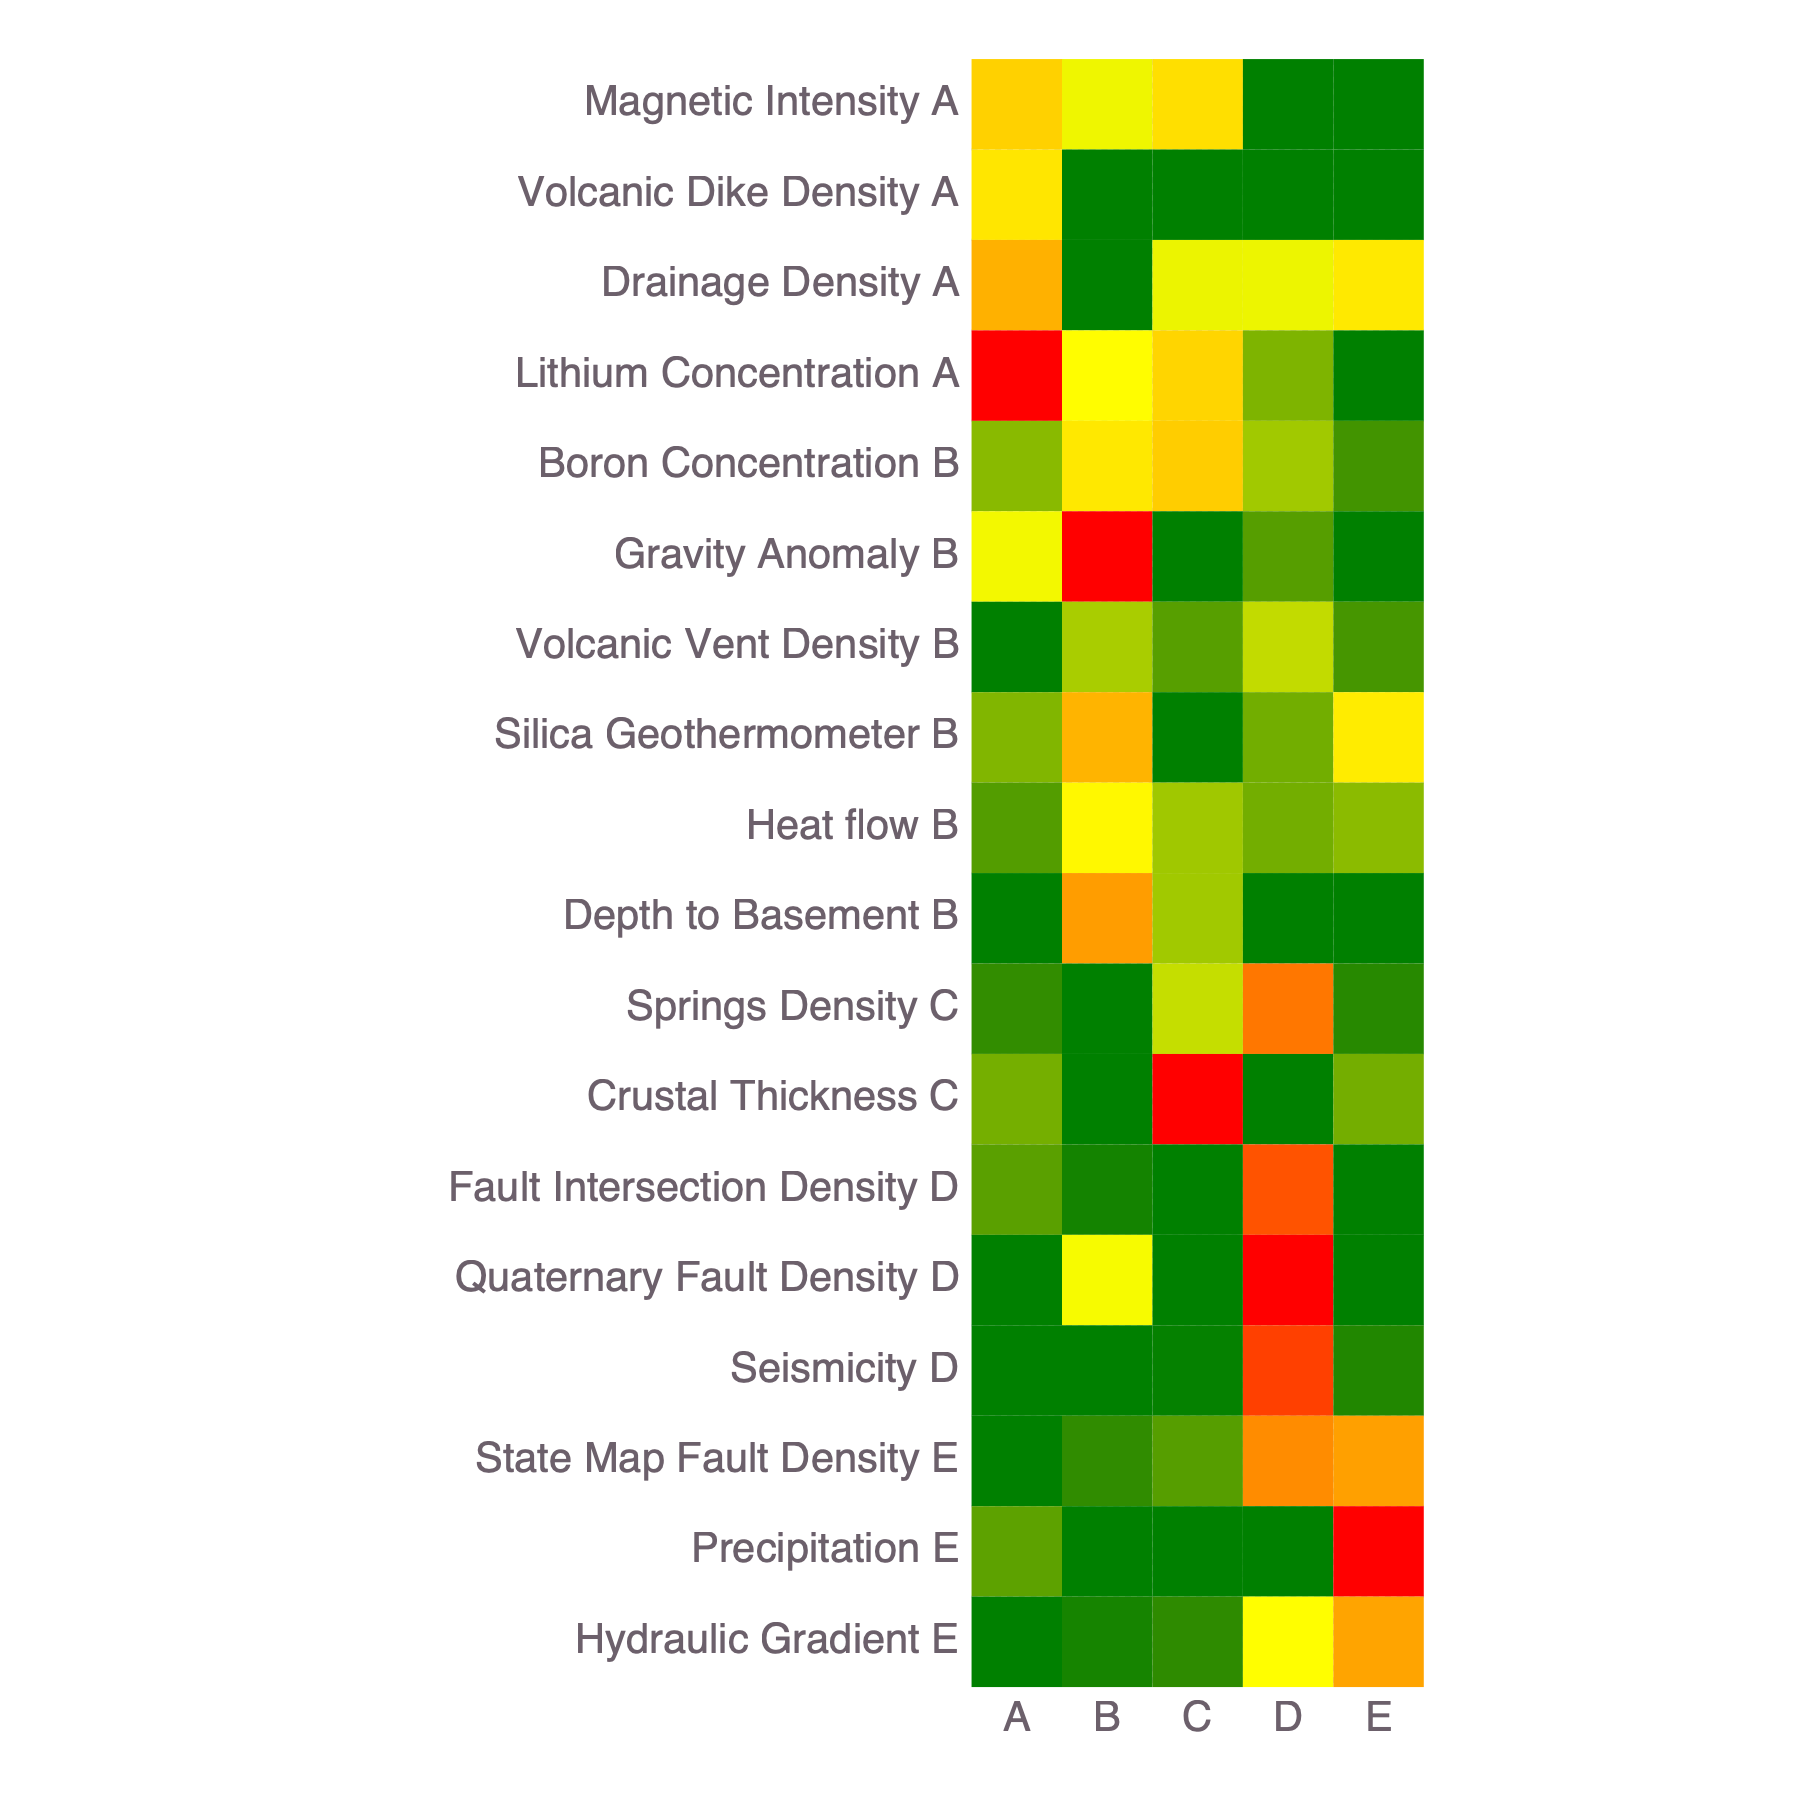
\includegraphics{../figures-case01/attributes-5-labeled-sorted.png}
\caption{attributes-5-labeled-sorted}
\end{figure}

The well locations are also clustered into \textbf{5} groups:

    \begin{tcolorbox}[breakable, size=fbox, boxrule=1pt, pad at break*=1mm,colback=cellbackground, colframe=cellborder]
\prompt{In}{incolor}{17}{\boxspacing}
\begin{Verbatim}[commandchars=\\\{\}]
\PY{n}{Mads}\PY{o}{.}\PY{n}{display}\PY{p}{(}\PY{l+s}{\PYZdq{}}\PY{l+s}{r}\PY{l+s}{e}\PY{l+s}{s}\PY{l+s}{u}\PY{l+s}{l}\PY{l+s}{t}\PY{l+s}{s}\PY{l+s}{\PYZhy{}}\PY{l+s}{c}\PY{l+s}{a}\PY{l+s}{s}\PY{l+s}{e}\PY{l+s}{0}\PY{l+s}{1}\PY{l+s}{/}\PY{l+s}{l}\PY{l+s}{o}\PY{l+s}{c}\PY{l+s}{a}\PY{l+s}{t}\PY{l+s}{i}\PY{l+s}{o}\PY{l+s}{n}\PY{l+s}{s}\PY{l+s}{\PYZhy{}}\PY{l+s}{5}\PY{l+s}{\PYZhy{}}\PY{l+s}{g}\PY{l+s}{r}\PY{l+s}{o}\PY{l+s}{u}\PY{l+s}{p}\PY{l+s}{s}\PY{l+s}{.}\PY{l+s}{t}\PY{l+s}{x}\PY{l+s}{t}\PY{l+s}{\PYZdq{}}\PY{p}{)}
\end{Verbatim}
\end{tcolorbox}

    \begin{Verbatim}[commandchars=\\\{\}]
Signal A (S1)
Ash spr         1.0
Allen spr       0.932
Mangas spr      0.883
Riverside well  0.834
Apache well     0.782
Spring Can      0.691
Turkey spr      0.678
Spring          0.677
Cliff spr       0.65
Warm spr        0.649
Garton well     0.617
Faywood spr     0.607
Kennecott well  0.599
Derry spr       0.578
Mimbres spr     0.565
Goat spr        0.37

Signal B (S4)
Fed H1 well     1.0
Well 4          0.848
Los Alturas     0.815
Well 2          0.789
Well 5          0.778
Lightning Dock  0.688
Carne well      0.627
Radium spr      0.626
Well 3          0.593
Victoria well   0.38

Signal C (S2)
Freiborn spr    1.0
Gila spr 1      0.78
Gila spr 2      0.696
Aragon spr      0.695
Ojo Caliente    0.36

Signal D (S3)
Jerry well      1.0
Pueblo well     0.971
Rainbow spr     0.943
Sacred spr      0.936
Dent well       0.927
Alamos spr      0.873
Laguna Pbl      0.855
Well 1          0.738

Signal E (S5)
Socorro Can     1.0
Ojitos spr      0.885
Ojo Canas       0.708
T or C spr      0.411
B.Iorio well    0.409

    \end{Verbatim}

    This grouping is based on analyses of the location matrix \texttt{H}:

\begin{figure}
\centering
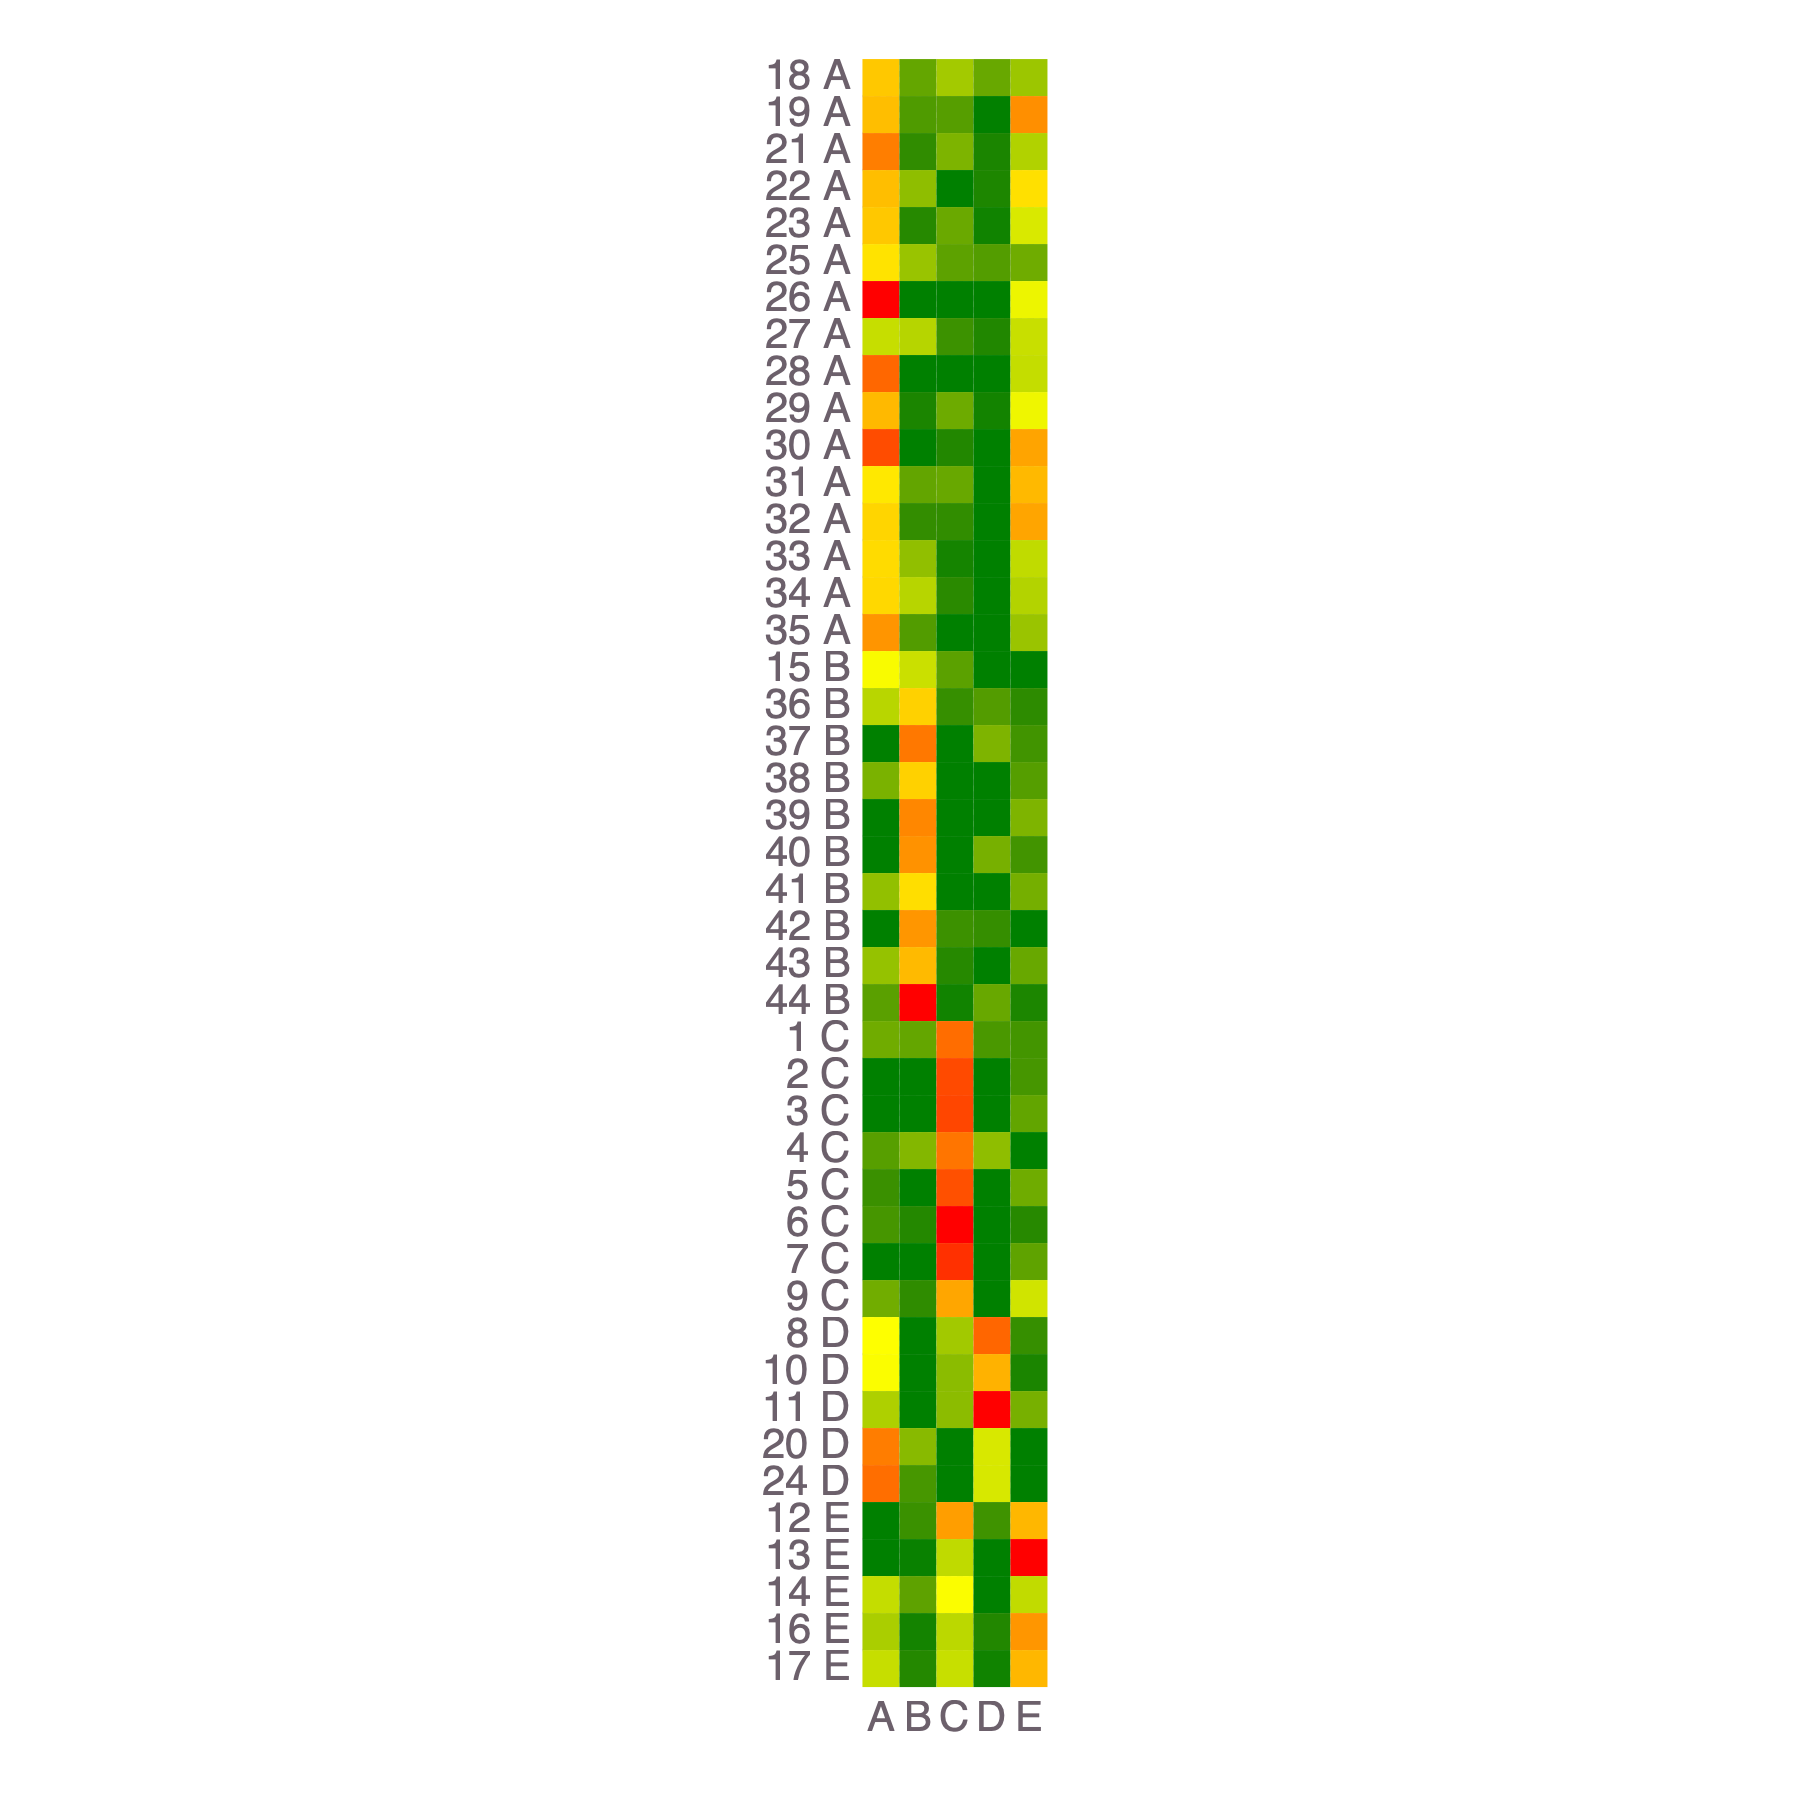
\includegraphics{../figures-case01/locations-5-labeled-sorted.png}
\caption{locations-5-labeled-sorted}
\end{figure}

The map \url{../figures-case01/locations-5-map.html} provides
interactive visualization of the extracted location groups (the html
file can also be opened within any browser).

    \hypertarget{comparison-of-the-ml-solutions-against-the-swnm-physiographic-provinces}{%
\paragraph{Comparison of the ML solutions against the SWNM physiographic
provinces}\label{comparison-of-the-ml-solutions-against-the-swnm-physiographic-provinces}}

The spatial association of the extracted signatures with the four
physiographic provinces in SWNM is summarized in the figure below:

\begin{figure}
\centering
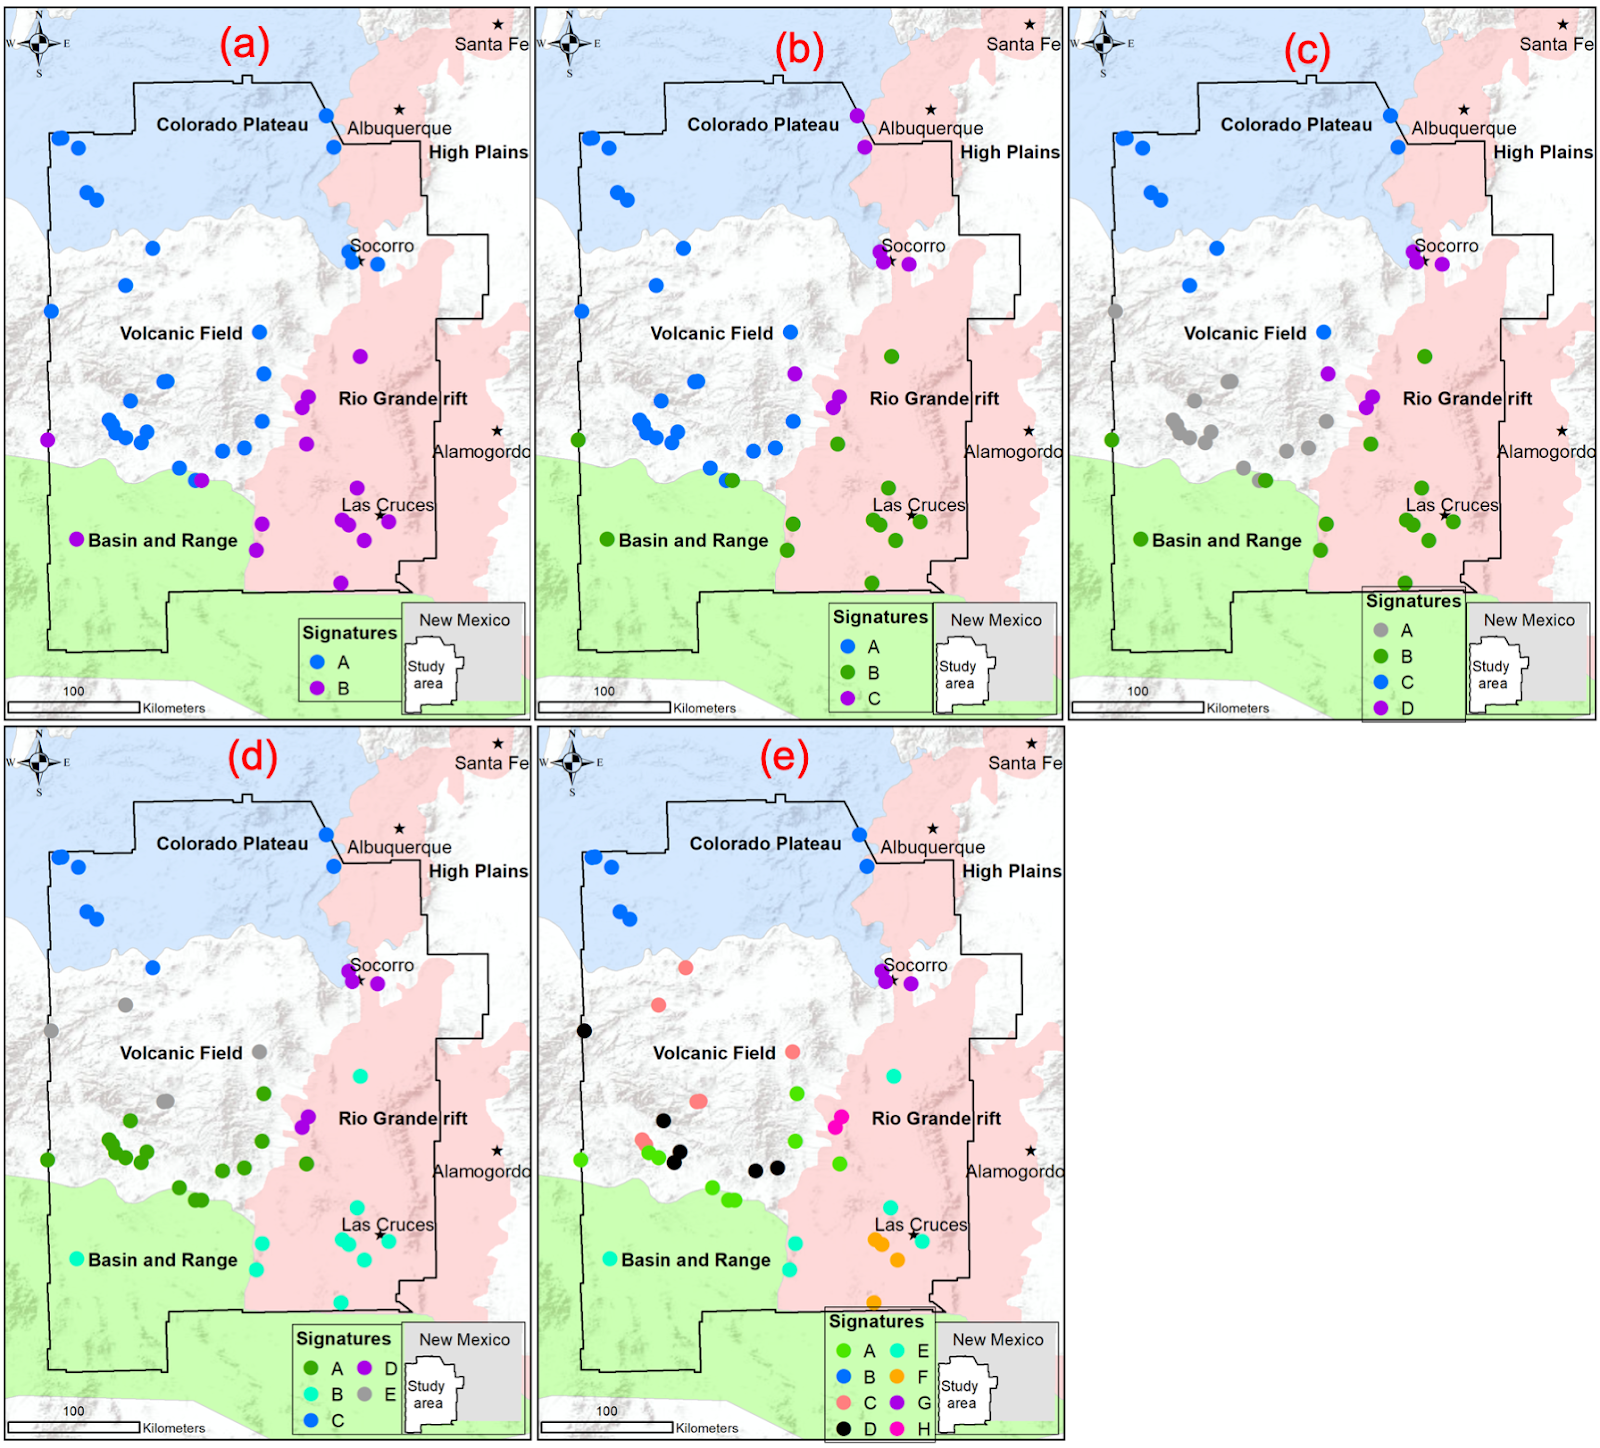
\includegraphics{../figures-case01/signatures.png}
\caption{signatures}
\end{figure}

The solutions for k=2, 3, and 4 provide a higher-level classification of
the geothermal locations, while the k=8 solution allow us to further
refine the geothermal signatures and their association to the
physiographic provinces. The solution for k=5 provides the best
classification of the geothermal locations.

Based on the figure above, it is clear that our ML algorithm was able to
blindly identify the physiographic provinces associated with analyzed
hydrogeothermal systems without providing any information about their
spatial location (coordinates).

Further observations based on the figure above are:

\begin{itemize}
\tightlist
\item
  The solution for k=2 separates the Colorado Plateau and the Volcanic
  Field (Signature A) from the Basin and Range and the Rift zone
  (Signature B) provinces (Figure a).
\item
  The k=3 solution combines the Colorado Plateau and the Volcanic Field
  in Signature A; however, Signatures B and C separate the Basin and
  Range and the Rio Grande Rift provinces, respectively (Figure b).
\item
  Signature A of the k=4 solution (Figure c) represents the Volcanic
  Field. Signature B captures the Basin and Range province. Signature C
  coincides with the Colorado Plateau. Signature D encompasses the Rio
  Grande Rift zone (Figure c).
\item
  The k=5 solution (Figure d) regroups the four signatures of the k=4
  solution into five signatures. Signatures A and E cover MDVF;
  Signatures B, C, and D capture the remaining three provinces: the
  Basin and Range, the Colorado Plateau, and the Rio Grande Rift
  provinces, respectively.
\item
  In the k=8 solution (Figure e), Signature B captures the Colorado
  Plateau province. Signatures G and H encompass two separate areas in
  the Rio Grande Rift zone (Figure e). Three of the signatures (A, C, D)
  are associated with the Volcanic Field capture spatial variability
  within this province. Two signatures (E and F) represent the spatial
  variability in the Basin and Range province.
\end{itemize}

    \hypertarget{description-of-location-matrices-w}{%
\paragraph{\texorpdfstring{Description of location matrices
(\texttt{W})}{Description of location matrices (W)}}\label{description-of-location-matrices-w}}

The plot below shows location matrices (\texttt{W}) of the extracted
signatures for all the accepted solutions together. From left to right,
the number of signatures increases. The matrices are color-coded to show
high (red) and low (green) associations between the locations and
signatures. Like the maps above, this figure below demonstrates how the
signatures get transformed and modified as the number of signatures
increases. The transitions of the signatures show the consistencies of
the obtained results.

\begin{figure}
\centering
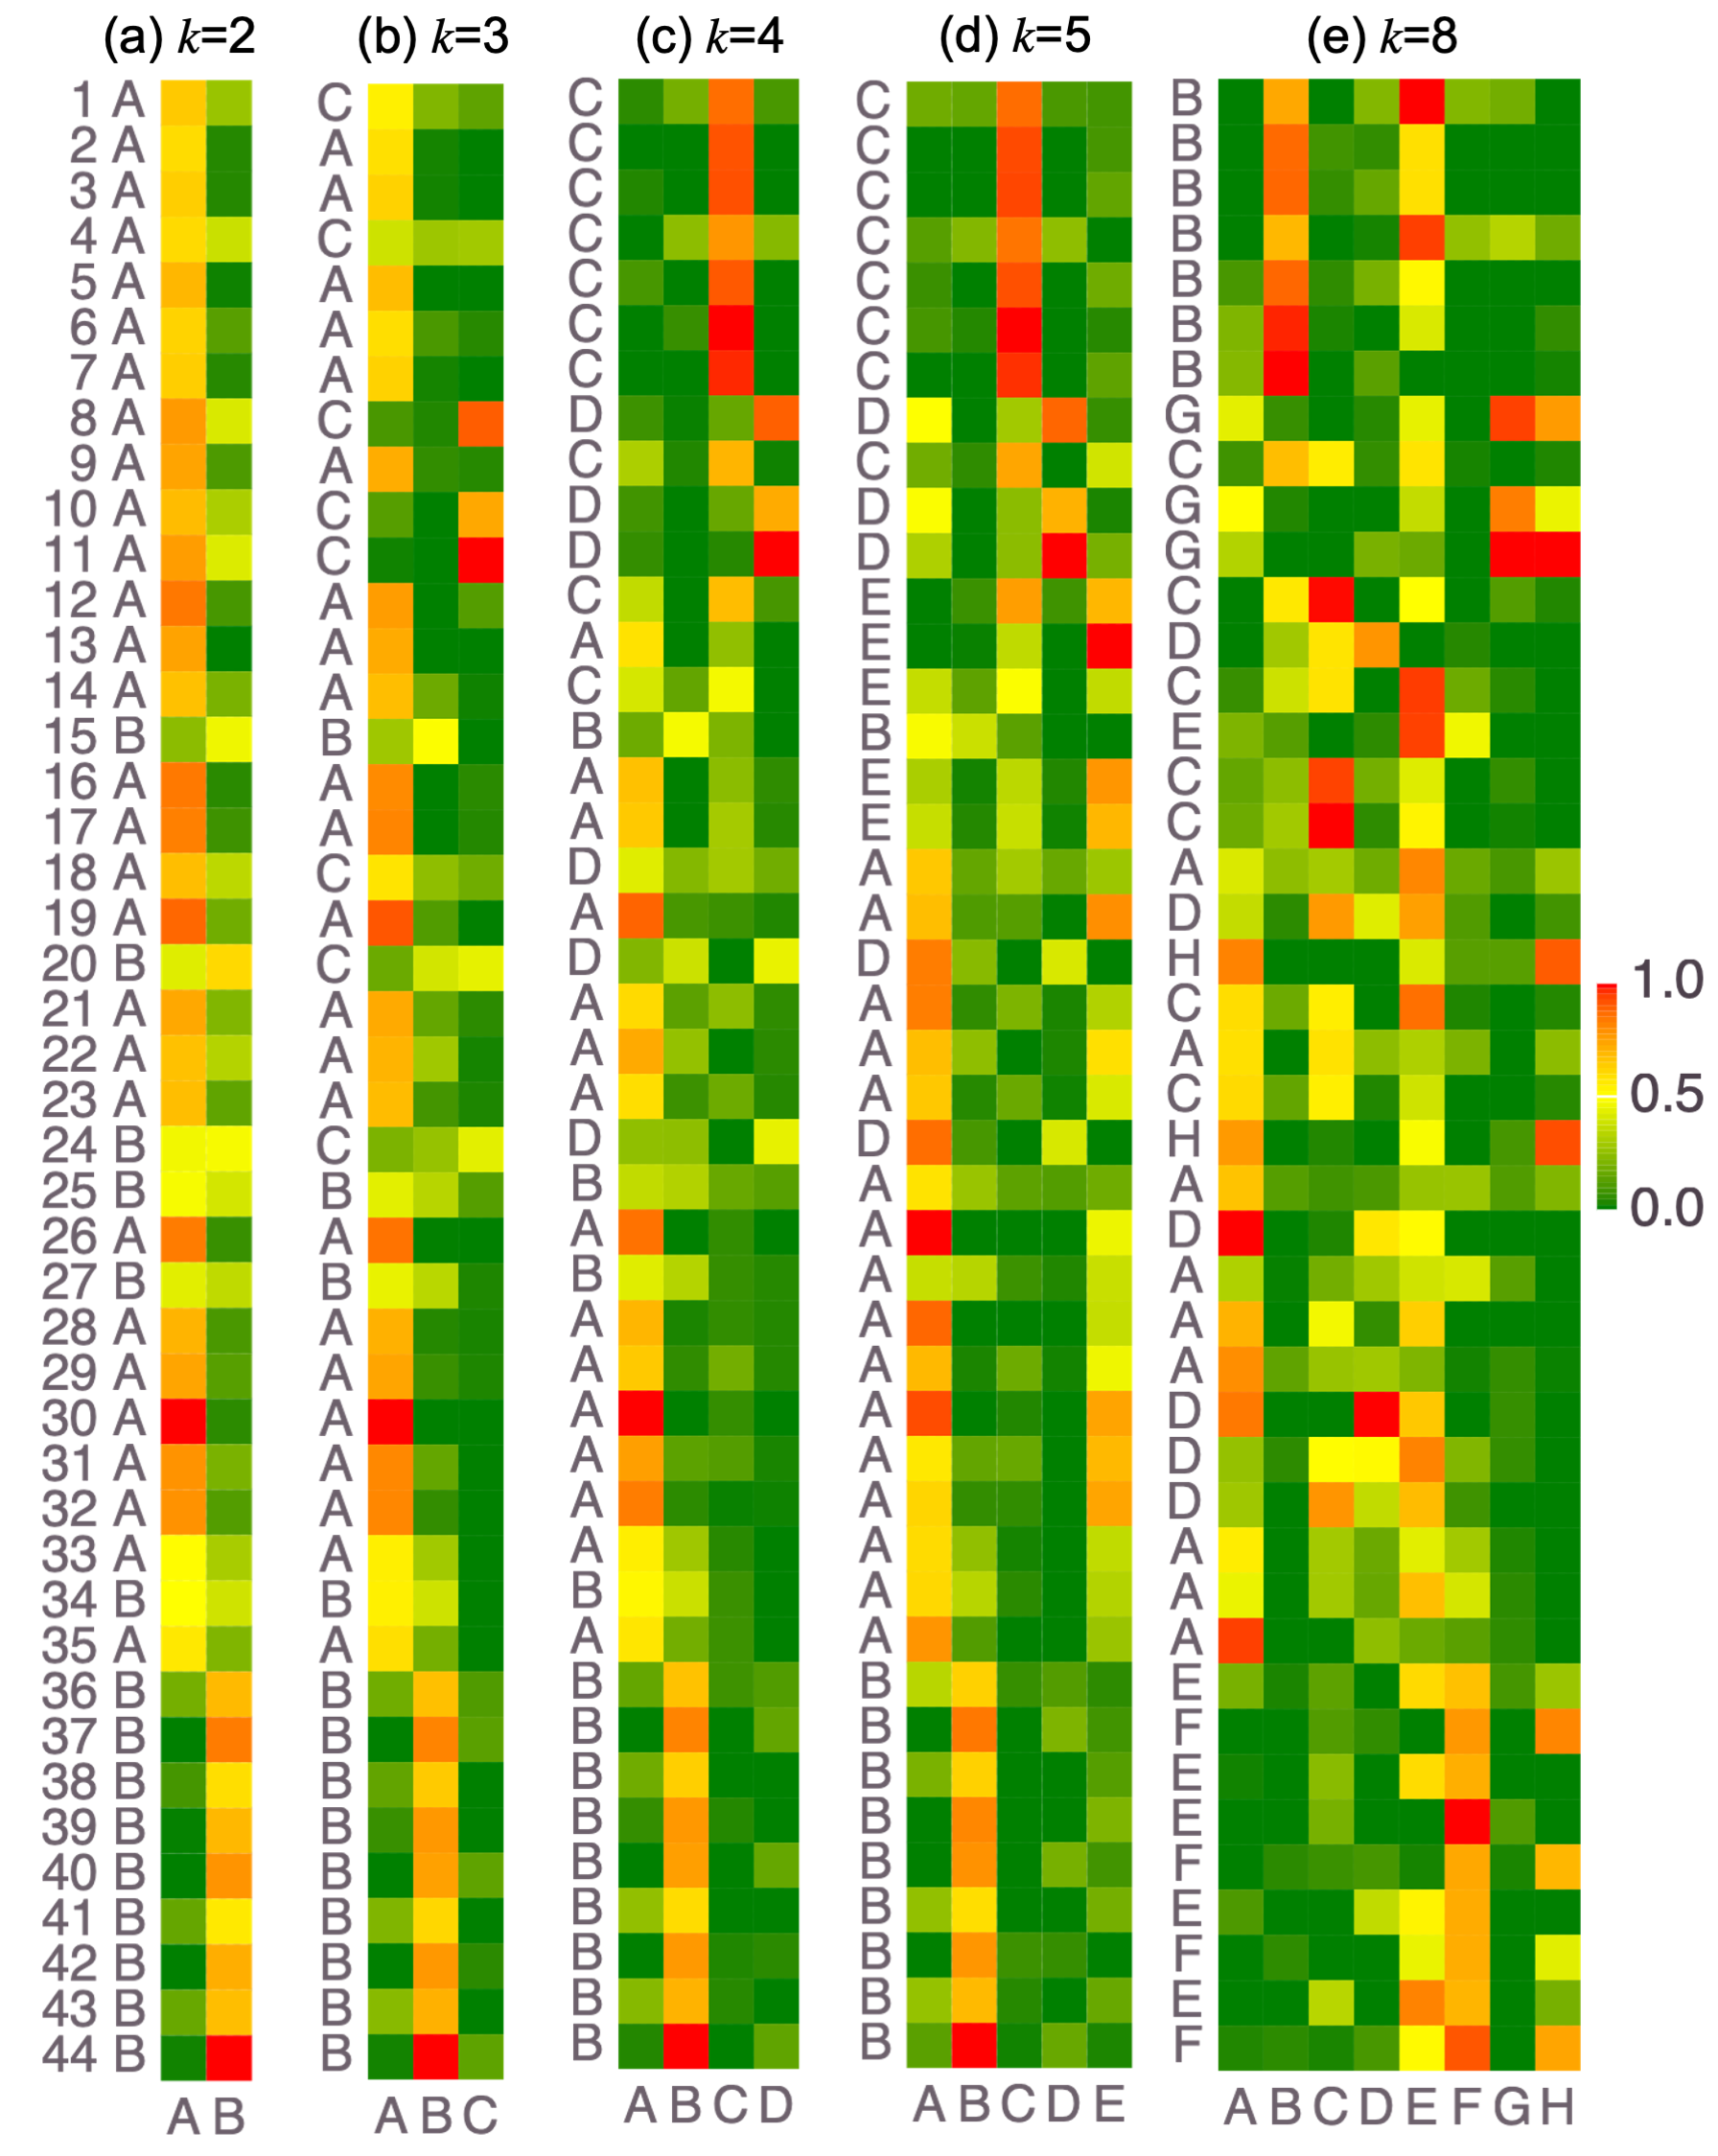
\includegraphics{../figures-case01/locations.png}
\caption{Ws}
\end{figure}

Further observations based on the figure above are (note that these
observations are consistent with the observations provided above
regarding the physiographic provinces):

\begin{itemize}
\tightlist
\item
  The k=2 solution subdivides the SWNM into two subregions.
\item
  Signatures A and B of the k=3 solution are split up into Signatures A,
  B, and C of the k=4 solution; however, Signature C of the k=3 solution
  and Signature D of the k=4 solution share very similar properties.
\item
  Signatures A, B, C, and D of both the k=4 and 5 solutions possess
  similar properties; however, the k=5 solution got a completely new
  signature (Signature E).
\item
  The k=8 solution regrouped the signatures of the k=5 solution.
  Signature A of the k=5 solution possesses similar properties to
  Signatures A and D of the k=8 solution. Signature B of the k=5
  solution shares similar properties to Signatures E and F of the k=8
  solution. Signature C of the k=5 solution has similar properties to
  both Signatures B and C of the k=8 solution. Signature D of the k=5
  solution and both Signatures G and H of the k=8 solution share similar
  properties.
\item
  It is critical to mention that although the 44 locations in the
  \texttt{W} matrices are labeled to be associated with a given
  geothermal signature (i.e., a certain region; A, B, etc.), it does not
  mean the locations are associated with only one signature as seen by
  the color-coding in the figure.
\item
  Instead, it means that those locations predominantly dominate
  commensurate signatures with contributions from other signatures too.
\end{itemize}

    \hypertarget{description-of-attribute-matrices-h}{%
\paragraph{\texorpdfstring{Description of attribute matrices
(\texttt{H})}{Description of attribute matrices (H)}}\label{description-of-attribute-matrices-h}}

The plot below shows attribute matrices of all the accepted solutions.
The number of signatures increases from left to right. The figure
demonstrates how each attribute contributes to the extracted signature.
The matrices are color-coded to show high (red) and low (green)
associations between the attributes and signatures. Also, this plot
shows how the signatures get transformed and modified as the number of
signatures increases. As above, the transitions of the signatures show
the consistencies of the obtained ML results.

\begin{figure}
\centering
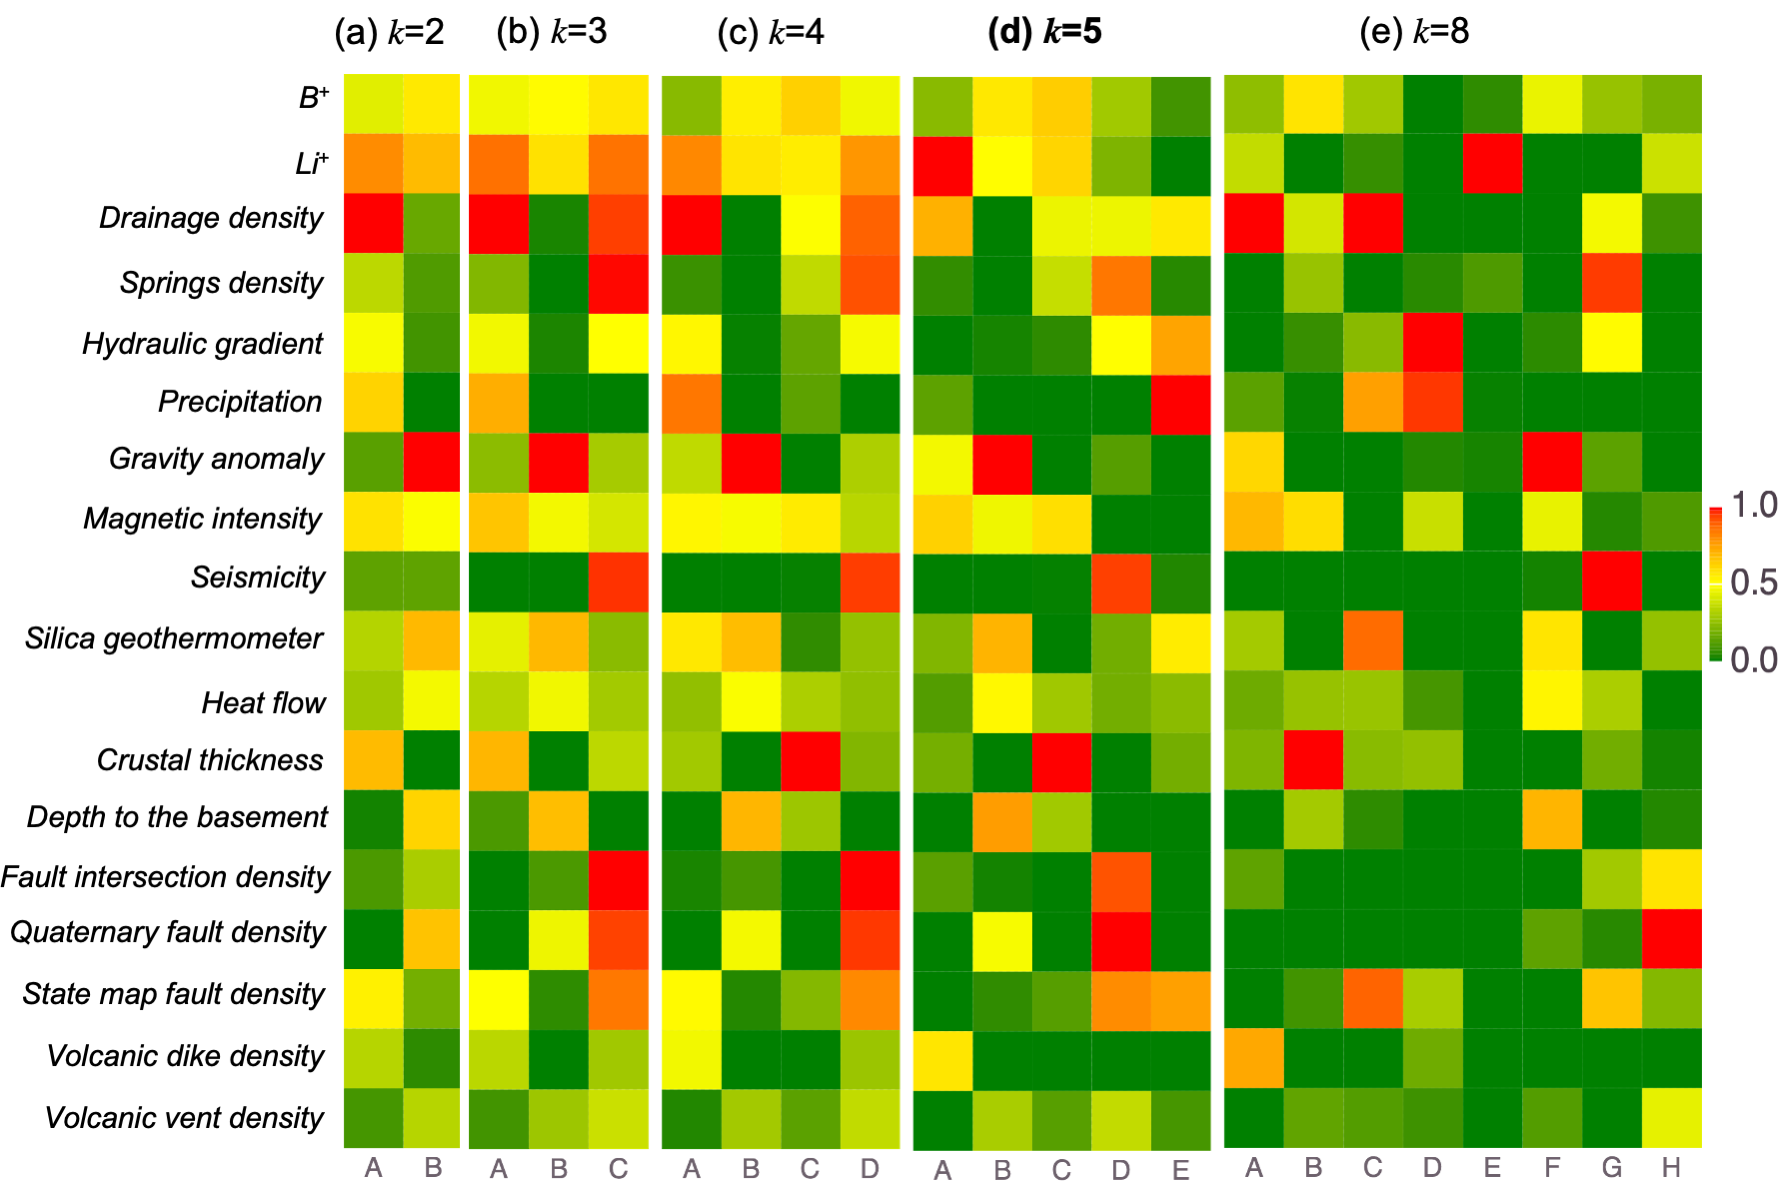
\includegraphics{../figures-case01/signals.png}
\caption{Hs}
\end{figure}

Further observations based on the figure above are:

\begin{itemize}
\tightlist
\item
  Signatures A, B, and C of the k=3 solution have similar properties to
  Signatures A, B, and both C and D of the k=4 solution, respectively.
\item
  Signatures of A, B, C, and D of the k=4 solution possess similar
  properties to signatures both A and E, B, C, and D of the k=5
  solution, respectively.
\item
  Signatures A, B, C, D, and E of the k=5 solution share similar
  properties to both A and E, F, B, both G and H, and both C and D of
  the k=8 solution, respectively.
\end{itemize}

    \hypertarget{optimal-geothermal-signatures-charecterizing-swnm-region}{%
\paragraph{Optimal geothermal signatures charecterizing SWNM
region}\label{optimal-geothermal-signatures-charecterizing-swnm-region}}

The figure below shows the map of the optimal signatures. The k=5
solution best characterizes the spatial associations and geothermal
attributes of the SWNM.

\begin{figure}
\centering
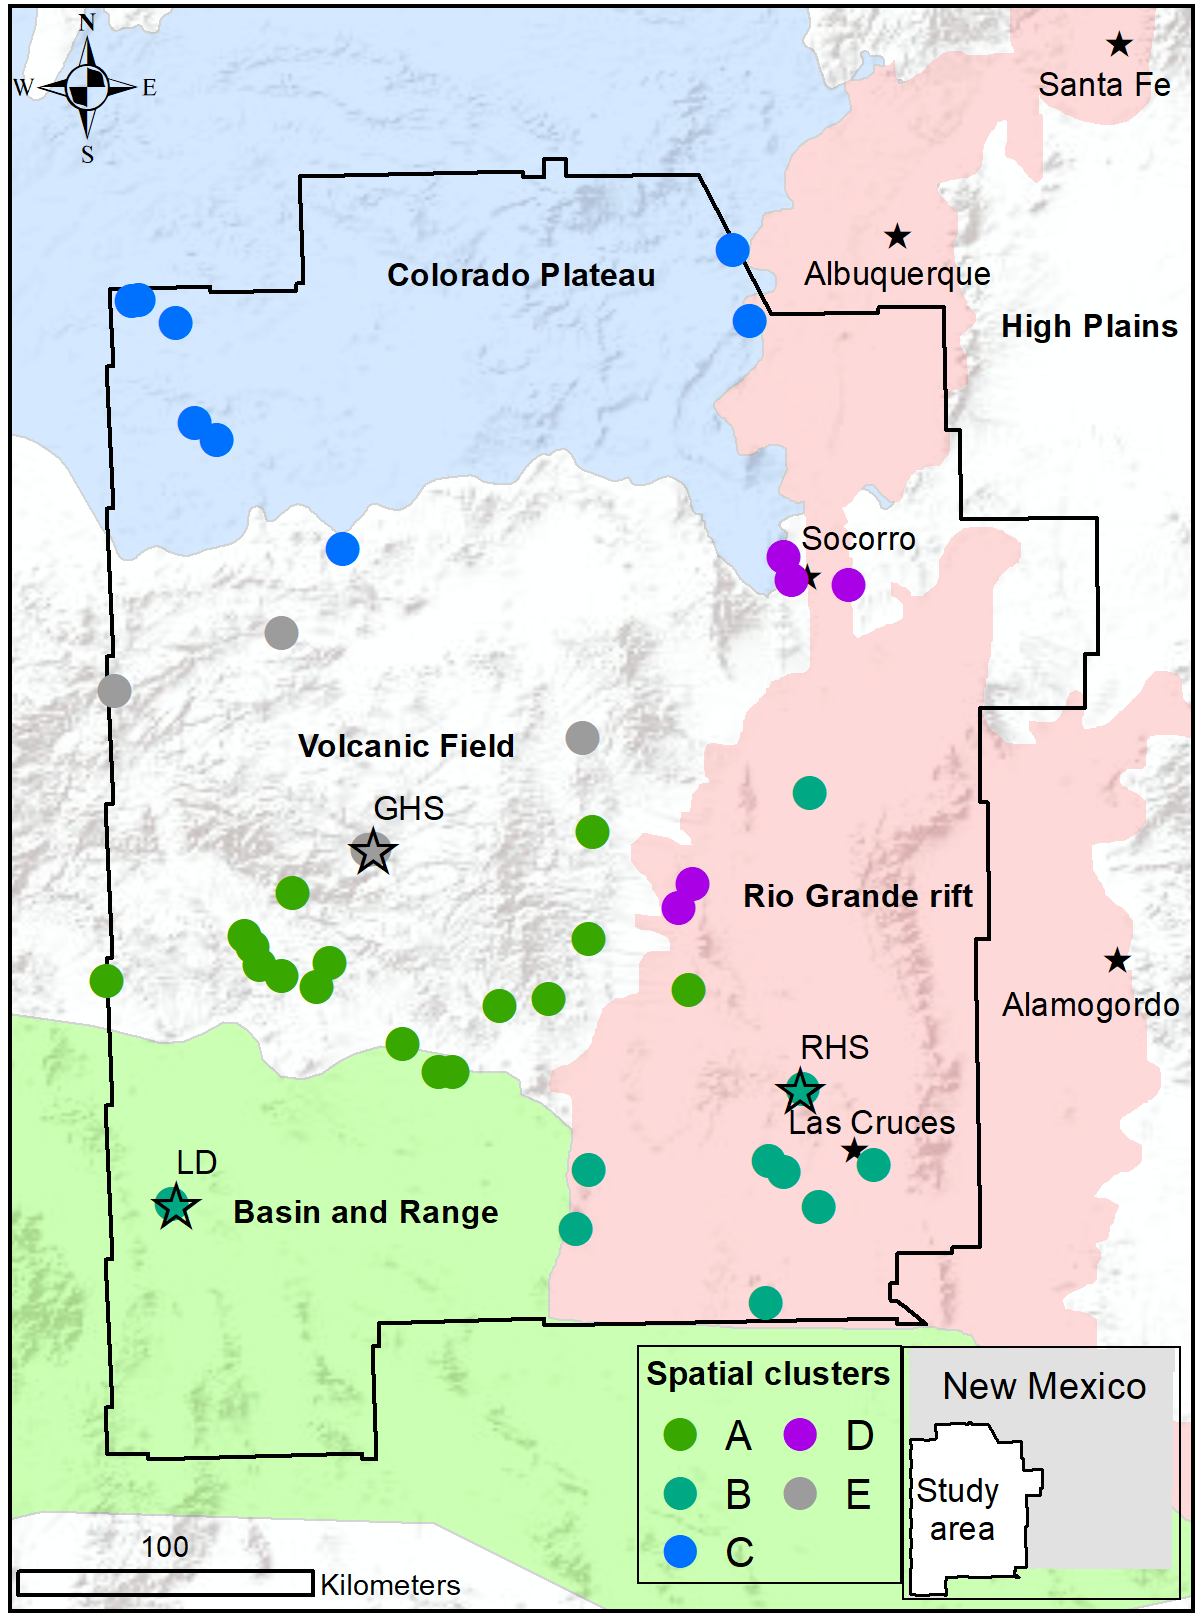
\includegraphics{../figures-case01/nmfk5.png}
\caption{Ws}
\end{figure}

    \hypertarget{signatures-and-their-relationships-to-resource-types-geothermal-attributes-physical-processes-and-physiographic-provinces}{%
\paragraph{Signatures and their relationships to resource types,
geothermal attributes, physical processes and physiographic
provinces}\label{signatures-and-their-relationships-to-resource-types-geothermal-attributes-physical-processes-and-physiographic-provinces}}

\begin{longtable}[]{@{}
  >{\raggedright\arraybackslash}p{(\columnwidth - 8\tabcolsep) * \real{0.16}}
  >{\raggedright\arraybackslash}p{(\columnwidth - 8\tabcolsep) * \real{0.21}}
  >{\raggedright\arraybackslash}p{(\columnwidth - 8\tabcolsep) * \real{0.21}}
  >{\raggedright\arraybackslash}p{(\columnwidth - 8\tabcolsep) * \real{0.21}}
  >{\raggedright\arraybackslash}p{(\columnwidth - 8\tabcolsep) * \real{0.21}}@{}}
\toprule
Signature & Resource type & Dominant attributes & Physical Significance
& Physiographci province \\
\midrule
\endhead
\bottomrule
\end{longtable}

\textbar A\textbar Low temperature\textbar{}

Gravity anomaly Magnetic intensity Volcanic dike density Drainage
density Li+ concentration

\textbar Shallow heat flow\textbar Southern MDVF\textbar{}
\textbar B\textbar Medium temperature\textbar{}

B+ and Li+ concentrations Gravity anomaly Magnetic intensity Quaternary
fault density Silica geothermometer Heat flow Depth to the basement

\textbar Deep heat flow\textbar Southern Rio Grande rift\textbar{}
\textbar C\textbar Low temperature\textbar{}

B+ and Li+ concentrations Magnetic intensity Drainage density Crustal
thickness

\textbar Deep heat source\textbar Colorado Plateau\textbar{}
\textbar D\textbar Low temperature\textbar{}

Drainage density Fault intersection density Seismicity State map fault
density Spring density Hydraulic gradient

\textbar Tectonics\textbar Northern Rio Grande Rift \textbar{}
\textbar E\textbar Medium temperature\textbar{}

Drainage density State map fault density Precipitation Silica
geothermometer Hydraulic gradient

\textbar Vertical hydraulics\textbar Northern MDVF\textbar{}

    \hypertarget{geothermal-resource-assessment}{%
\paragraph{Geothermal resource
assessment}\label{geothermal-resource-assessment}}

\begin{itemize}
\tightlist
\item
  The extracted signatures characterize low- and medium-temperature
  hydrothermal systems.
\item
  The signatures are characterized by unique geothermal attributes which
  are automatically identified by our ML analyses.
\end{itemize}

\hypertarget{medium-temperature-hydrothermal-systems}{%
\subparagraph{Medium-temperature hydrothermal
systems}\label{medium-temperature-hydrothermal-systems}}

\begin{itemize}
\tightlist
\item
  Two of the signatures (B and E) represent medium-temperature
  hydrothermal systems
\item
  The medium-temperature signatures (B and E) fall in the Southern Rio
  Grande Rift and the Northern MDVF zones.

  \begin{itemize}
  \tightlist
  \item
    The dominant attributes of the Southern Rio Grande Rift zone are B+
    and Li+ concentrations, Gravity anomaly, Magnetic intensity,
    Quaternary fault density, Silica geothermometer, Heat flow, Depth to
    the basement.
  \item
    The dominant attributes of the Northern MDVF are Drainage density,
    State map fault density, Precipitation, Silica geothermometer,
    Hydraulic gradient.
  \end{itemize}
\end{itemize}

\hypertarget{low-temperature-hydrothermal-systems}{%
\subparagraph{Low-temperature hydrothermal
systems}\label{low-temperature-hydrothermal-systems}}

\begin{itemize}
\tightlist
\item
  Three of the signatures (A, C, and D) represent low-temperature
  hydrothermal systems.
\item
  The low-temperature signatures (A, C, and D) fall in the Southern
  MDVF, Colorado Plateau, and Northern Rio Grande Rift zones.
\end{itemize}

For more details, please look at our paper titled: ``Discovering Hidden
Geothermal Signatures using Unsupervised Machine Learning.''


    % Add a bibliography block to the postdoc
    
    
    
\end{document}
